\documentclass[11pt]{article}

    % --- Paquetes de Formato de Informe ---
    \usepackage[utf8]{inputenc}
    \usepackage[spanish, es-tabla]{babel} % Traducción a español
    \usepackage{fancyhdr} % Encabezados y pies de página
    \usepackage{lastpage} % Para indicar el total de páginas
    \usepackage{titlesec} % Para dar formato a los títulos
    
    % --- Paquetes originales mantenidos ---
    \usepackage[breakable]{tcolorbox}
    \usepackage{parskip} 
    \usepackage{graphicx}
    \setkeys{Gin}{keepaspectratio}
    \usepackage{caption}
    \DeclareCaptionFormat{nocaption}{}
    \captionsetup{format=nocaption,aboveskip=0pt,belowskip=0pt}
    \usepackage{float}
    \floatplacement{figure}{H} 
    \usepackage{xcolor} 
    \usepackage{enumerate} 
    \usepackage{geometry} 
    \usepackage{amsmath} 
    \usepackage{amssymb} 
    \usepackage{textcomp} 
    \usepackage{upquote} 
    \usepackage{eurosym} 
    \usepackage{iftex}
    \usepackage{fancyvrb} 
    \usepackage{grffile} 
    \usepackage[Export]{adjustbox} 
    \adjustboxset{max size={0.9\linewidth}{0.9\paperheight}}
    \usepackage{longtable} 
    \usepackage{booktabs}  
    \usepackage{array}     
    \usepackage{calc}      
    \usepackage[inline]{enumitem} 
    \usepackage[normalem]{ulem} 
    \usepackage{soul}      
    \usepackage{mathrsfs}

    % --- Configuración de Márgenes ---
    \geometry{tmargin=1in,bmargin=1in,lmargin=1in,rmargin=1in, headheight=14pt}

    % --- Configuración de Encabezado y Pie de Página ---
    \pagestyle{fancy}
    \fancyhf{}
    \lhead{\footnotesize Resolución Numérica de la Ecuación de Schrödinger}
    \rhead{\footnotesize Informe de Práctica}
    \rfoot{\footnotesize Página \thepage\ de \pageref{LastPage}}
    \lfoot{\footnotesize Métodos Numéricos y Aplicaciones a la Física}
    \renewcommand{\headrulewidth}{0.4pt}
    \renewcommand{\footrulewidth}{0.4pt}

    % --- Configuración de Hyperref (debe ir al final) ---
    \usepackage{hyperref}
    \definecolor{urlcolor}{rgb}{0,.145,.698}
    \definecolor{linkcolor}{rgb}{.71,0.21,0.01}
    \definecolor{citecolor}{rgb}{.12,.54,.11}
    \hypersetup{
      breaklinks=true,
      colorlinks=true,
      urlcolor=urlcolor,
      linkcolor=linkcolor,
      citecolor=citecolor,
    }

    % Hack Pygments
    \AtBeginDocument{\def\PYZsq{\textquotesingle}}

    % Definiciones de Colores ANSI y Pygments (Mantenidas del original)
    \definecolor{ansi-black}{HTML}{3E424D}
    \definecolor{ansi-black-intense}{HTML}{282C36}
    \definecolor{ansi-red}{HTML}{E75C58}
    \definecolor{ansi-red-intense}{HTML}{B22B31}
    \definecolor{ansi-green}{HTML}{00A250}
    \definecolor{ansi-green-intense}{HTML}{007427}
    \definecolor{ansi-yellow}{HTML}{DDB62B}
    \definecolor{ansi-yellow-intense}{HTML}{B27D12}
    \definecolor{ansi-blue}{HTML}{208FFB}
    \definecolor{ansi-blue-intense}{HTML}{0065CA}
    \definecolor{ansi-magenta}{HTML}{D160C4}
    \definecolor{ansi-magenta-intense}{HTML}{A03196}
    \definecolor{ansi-cyan}{HTML}{60C6C8}
    \definecolor{ansi-cyan-intense}{HTML}{258F8F}
    \definecolor{ansi-white}{HTML}{C5C1B4}
    \definecolor{ansi-white-intense}{HTML}{A1A6B2}
    \definecolor{ansi-default-inverse-fg}{HTML}{FFFFFF}
    \definecolor{ansi-default-inverse-bg}{HTML}{000000}
    \definecolor{outerrorbackground}{HTML}{FFDFDF}

    \providecommand{\tightlist}{\setlength{\itemsep}{0pt}\setlength{\parskip}{0pt}}
    \DefineVerbatimEnvironment{Highlighting}{Verbatim}{commandchars=\\\{\}}
    \newenvironment{Shaded}{}{}
    \newcommand{\KeywordTok}[1]{\textcolor[rgb]{0.00,0.44,0.13}{\textbf{{#1}}}}
    \newcommand{\DataTypeTok}[1]{\textcolor[rgb]{0.56,0.13,0.00}{{#1}}}
    \newcommand{\DecValTok}[1]{\textcolor[rgb]{0.25,0.63,0.44}{{#1}}}
    \newcommand{\BaseNTok}[1]{\textcolor[rgb]{0.25,0.63,0.44}{{#1}}}
    \newcommand{\FloatTok}[1]{\textcolor[rgb]{0.25,0.63,0.44}{{#1}}}
    \newcommand{\CharTok}[1]{\textcolor[rgb]{0.25,0.44,0.63}{{#1}}}
    \newcommand{\StringTok}[1]{\textcolor[rgb]{0.25,0.44,0.63}{{#1}}}
    \newcommand{\CommentTok}[1]{\textcolor[rgb]{0.38,0.63,0.69}{\textit{{#1}}}}
    \newcommand{\OtherTok}[1]{\textcolor[rgb]{0.00,0.44,0.13}{{#1}}}
    \newcommand{\AlertTok}[1]{\textcolor[rgb]{1.00,0.00,0.00}{\textbf{{#1}}}}
    \newcommand{\FunctionTok}[1]{\textcolor[rgb]{0.02,0.16,0.49}{{#1}}}
    \newcommand{\RegionMarkerTok}[1]{{#1}}
    \newcommand{\ErrorTok}[1]{\textcolor[rgb]{1.00,0.00,0.00}{\textbf{{#1}}}}
    \newcommand{\NormalTok}[1]{{#1}}
    \newcommand{\ConstantTok}[1]{\textcolor[rgb]{0.53,0.00,0.00}{{#1}}}
    \newcommand{\SpecialCharTok}[1]{\textcolor[rgb]{0.25,0.44,0.63}{{#1}}}
    \newcommand{\VerbatimStringTok}[1]{\textcolor[rgb]{0.25,0.44,0.63}{{#1}}}
    \newcommand{\SpecialStringTok}[1]{\textcolor[rgb]{0.73,0.40,0.53}{{#1}}}
    \newcommand{\ImportTok}[1]{{#1}}
    \newcommand{\DocumentationTok}[1]{\textcolor[rgb]{0.73,0.13,0.13}{\textit{{#1}}}}
    \newcommand{\AnnotationTok}[1]{\textcolor[rgb]{0.38,0.63,0.69}{\textbf{\textit{{#1}}}}}
    \newcommand{\CommentVarTok}[1]{\textcolor[rgb]{0.38,0.63,0.69}{\textbf{\textit{{#1}}}}}
    \newcommand{\VariableTok}[1]{\textcolor[rgb]{0.10,0.09,0.49}{{#1}}}
    \newcommand{\ControlFlowTok}[1]{\textcolor[rgb]{0.00,0.44,0.13}{\textbf{{#1}}}}
    \newcommand{\OperatorTok}[1]{\textcolor[rgb]{0.40,0.40,0.40}{{#1}}}
    \newcommand{\BuiltInTok}[1]{{#1}}
    \newcommand{\ExtensionTok}[1]{{#1}}
    \newcommand{\PreprocessorTok}[1]{\textcolor[rgb]{0.74,0.48,0.00}{{#1}}}
    \newcommand{\AttributeTok}[1]{\textcolor[rgb]{0.49,0.56,0.16}{{#1}}}
    \newcommand{\InformationTok}[1]{\textcolor[rgb]{0.38,0.63,0.69}{\textbf{\textit{{#1}}}}}
    \newcommand{\WarningTok}[1]{\textcolor[rgb]{0.38,0.63,0.69}{\textbf{\textit{{#1}}}}}

    \makeatletter
    \newsavebox\pandoc@box
    \newcommand*\pandocbounded[1]{%
      \sbox\pandoc@box{#1}%
      \Gscale@div\@tempa\textheight{\dimexpr\ht\pandoc@box+\dp\pandoc@box\relax}%
      \Gscale@div\@tempb\linewidth{\wd\pandoc@box}%
      \ifdim\@tempb\p@<\@tempa\p@ \let\@tempa\@tempb \fi
      \ifdim\@tempa\p@<\p@ \scalebox{\@tempa}{\usebox\pandoc@box}%
      \else \usebox{\pandoc@box} \fi
    }
    \makeatother

    \def\br{\hspace*{\fill} \\* }
    \def\gt{>}
    \def\lt{<}
    \let\Oldtex\TeX
    \let\Oldlatex\LaTeX
    \renewcommand{\TeX}{\textrm{\Oldtex}}
    \renewcommand{\LaTeX}{\textrm{\Oldlatex}}

    % Pygments definitions
    \makeatletter
    \def\PY@reset{\let\PY@it=\relax \let\PY@bf=\relax \let\PY@ul=\relax \let\PY@tc=\relax \let\PY@bc=\relax \let\PY@ff=\relax}
    \def\PY@tok#1{\csname PY@tok@#1\endcsname}
    \def\PY@toks#1+{\ifx\relax#1\empty\else \PY@tok{#1}\expandafter\PY@toks\fi}
    \def\PY@do#1{\PY@bc{\PY@tc{\PY@ul{\PY@it{\PY@bf{\PY@ff{#1}}}}}}}
    \def\PY#1#2{\PY@reset\PY@toks#1+\relax+\PY@do{#2}}
    \@namedef{PY@tok@w}{\def\PY@tc##1{\textcolor[rgb]{0.73,0.73,0.73}{##1}}}
    \@namedef{PY@tok@c}{\let\PY@it=\textit\def\PY@tc##1{\textcolor[rgb]{0.24,0.48,0.48}{##1}}}
    \@namedef{PY@tok@k}{\let\PY@bf=\textbf\def\PY@tc##1{\textcolor[rgb]{0.00,0.50,0.00}{##1}}}
    \@namedef{PY@tok@o}{\def\PY@tc##1{\textcolor[rgb]{0.40,0.40,0.40}{##1}}}
    \@namedef{PY@tok@nb}{\def\PY@tc##1{\textcolor[rgb]{0.00,0.50,0.00}{##1}}}
    \@namedef{PY@tok@nf}{\def\PY@tc##1{\textcolor[rgb]{0.00,0.00,1.00}{##1}}}
    \@namedef{PY@tok@s}{\def\PY@tc##1{\textcolor[rgb]{0.73,0.13,0.13}{##1}}}
    \@namedef{PY@tok@m}{\def\PY@tc##1{\textcolor[rgb]{0.40,0.40,0.40}{##1}}}
    \@namedef{PY@tok@sa}{\def\PY@tc##1{\textcolor[rgb]{0.73,0.13,0.13}{##1}}}
    \def\PYZbs{\char`\\} \def\PYZus{\char`\_} \def\PYZob{\char`\{} \def\PYZcb{\char`\}} \def\PYZca{\char`\^} \def\PYZam{\char`\&} \def\PYZlt{\char`\<} \def\PYZgt{\char`\>} \def\PYZsh{\char`\#} \def\PYZpc{\char`\%} \def\PYZdl{\char`\$} \def\PYZhy{\char`\-} \def\PYZsq{\char`\'} \def\PYZdq{\char`\"} \def\PYZti{\char`\~}
    \makeatother

    \makeatletter
    \newbox\Wrappedcontinuationbox
    \newbox\Wrappedvisiblespacebox
    \newcommand*\Wrappedvisiblespace {\textcolor{red}{\textvisiblespace}}
    \newcommand*\Wrappedcontinuationsymbol {\textcolor{red}{\llap{\tiny$\m@th\hookrightarrow$}}}
    \newcommand*\Wrappedcontinuationindent {3ex }
    \newcommand*\Wrappedafterbreak {\kern\Wrappedcontinuationindent\copy\Wrappedcontinuationbox}
    \newcommand*\Wrappedbreaksatspecials {%
        \def\PYGZus{\discretionary{\char`\_}{\Wrappedafterbreak}{\char`\_}}%
        \def\PYGZob{\discretionary{}{\Wrappedafterbreak\char`\{}{\char`\{}}%
        \def\PYGZcb{\discretionary{\char`\}}{\Wrappedafterbreak}{\char`\}}}%
    }
    \makeatother

    \let\OriginalVerbatim=\Verbatim
    \makeatletter
    \renewcommand{\Verbatim}[1][1]{%
        \sbox\Wrappedcontinuationbox {\Wrappedcontinuationsymbol}%
        \sbox\Wrappedvisiblespacebox {\FV@SetupFont\Wrappedvisiblespace}%
        \def\FancyVerbFormatLine ##1{\hsize\linewidth
            \vtop{\raggedright\hyphenpenalty\z@\exhyphenpenalty\z@
                \doublehyphendemerits\z@\finalhyphendemerits\z@
                \strut ##1\strut}%
        }%
        \def\FV@Space {%
            \nobreak\hskip\z@ plus\fontdimen3\font minus\fontdimen4\font
            \discretionary{\copy\Wrappedvisiblespacebox}{\Wrappedafterbreak}
            {\kern\fontdimen2\font}%
        }%
        \Wrappedbreaksatspecials
        \OriginalVerbatim[#1]%
    }
    \makeatother

    \definecolor{incolor}{HTML}{303F9F}
    \definecolor{outcolor}{HTML}{D84315}
    \definecolor{cellborder}{HTML}{CFCFCF}
    \definecolor{cellbackground}{HTML}{F7F7F7}
    \makeatletter
    \newcommand{\boxspacing}{\kern\kvtcb@left@rule\kern\kvtcb@boxsep}
    \makeatother
    \newcommand{\prompt}[4]{{\ttfamily\llap{{\color{#2}[#3]:\hspace{3pt}#4}}\vspace{-\baselineskip}}}

    \sloppy

% ==============================================================================
% COMIENZO DEL DOCUMENTO
% ==============================================================================
\begin{document}

% --- PORTADA ---
\begin{titlepage}
    \centering
    \vspace*{2cm}
    {\scshape\Large Métodos Numéricos y sus Aplicaciones a la Física \par}
    \vspace{1.5cm}
    {\huge\bfseries Resolución Numérica de la Ecuación de Schrödinger: Del Pozo de Potencial a los Átomos Multielectrónicos \par}
    \vspace{2cm}
    {\Large\textbf{Autor:}\par}
    {\Large  Edgar Fernández Vigil\par}
    \vfill
    {\large \today \par}
\end{titlepage}

% --- ÍNDICE ---
\newpage
\tableofcontents
\newpage

% --- CONTENIDO ---
\section*{Resumen inicial}
\addcontentsline{toc}{section}{Resumen inicial}
Este informe presenta la resolución numérica de la ecuación de Schrödinger independiente del tiempo para tres escenarios de complejidad creciente: pozo de potencial finito (1D), átomos hidrogenoides (H y $He^+$) y litio efectivo con apantallamiento.

Se comparan dos estrategias de integración (disparo explícito y Numerov), y se evalúan precisión, estabilidad y sensibilidad a parámetros numéricos (paso de malla, tolerancia de bisección y tamaño de dominio). Los resultados se muestran como salida de terminal y se interpretan físicamente en la discusión final.

Las conclusiones principales son: (i) Numerov ofrece mejor precisión y robustez para el mismo costo de orden de magnitud; (ii) las energías de H y $He^+$ reproducen correctamente el comportamiento analítico esperado; (iii) en litio efectivo se observa ruptura de degeneración entre estados $s$ y $p$ debido a penetración y apantallamiento.

\section{Objetivos y alcance}
Los objetivos de la práctica son:
\begin{enumerate}
    \item Implementar métodos numéricos para obtener autovalores y autofunciones de la ecuación de Schrödinger.
    \item Validar la implementación frente a casos de referencia con solución conocida.
    \item Analizar limitaciones numéricas y su impacto en la interpretación física de los resultados.
\end{enumerate}

El alcance incluye sistemas de un electrón y un modelo efectivo de litio, sin incorporar correlación electrónica completa ni correcciones relativistas.

\section{Introducción teórica y pozo de potencial finito (1D)}\label{introducciuxf3n-teuxf3rica-y-pozo-de-potencial-finito-1d}

La ecuación de Schrödinger describe la evolución temporal y espacial de
una partícula masiva no relativista. Para sistemas donde el potencial
\(V\) no depende del tiempo, la función de onda se puede factorizar,
conduciendo a la ecuación de Schrödinger independiente del tiempo:
\[-\frac{\hbar^2}{2m}\frac{d^2\psi(x)}{dx^2} + V(x)\psi(x) = E\psi(x)\]

El objetivo principal de la física computacional en este ámbito es
encontrar los autovalores de energía permitidos (\(E_n\)) y sus
correspondientes autofunciones (\(\psi_n\)) para los estados ligados del
sistema. Reordenando la ecuación, obtenemos una ecuación diferencial de
segundo orden homogénea:
\[\frac{d^2\psi(x)}{dx^2} = \frac{2m}{\hbar^2}(V(x) - E)\psi(x)\]

Consideramos primero una partícula confinada en un pozo de potencial de
anchura \(a\) y profundidad \(V_0\). El potencial se define como:
\[V(x) = \begin{cases} V_0 & \text{si } |x| > a/2 \\ 0 & \text{si } |x| < a/2 \end{cases}\]

Para facilitar el tratamiento numérico en el ordenador y evitar el
manejo de constantes muy pequeñas, aplicamos un cambio de escala
definiendo la variable adimensional \(u = x/a\). Aplicando la regla de
la cadena, la derivada se transforma en
\(\frac{d}{dx} = \frac{1}{a}\frac{d}{du}\). Sustituyendo en la ecuación
original:
\[\frac{d^2\psi(u)}{du^2} = \frac{2ma^2}{\hbar^2}[V(u) - E]\psi(u)\]

A continuación, definimos una constante adimensional del sistema
\(k = \frac{2ma^2V_0}{\hbar^2}\) y parametrizamos la energía en función
de la profundidad del pozo como \(\alpha = E/V_0\). Con estas
definiciones, la ecuación se reduce a una forma compacta computable:
\[\psi''(u) = C(u)\psi(u)\] Donde \(C(u)\) encapsula la física del
problema de forma discreta:

\[
C(u) = k\left(\frac{V(u)}{V_0} - \alpha\right)
\]

Para el pozo finito utilizado, con región interna \(|u|<1/2\) y externa
\(|u|\geq 1/2\), se obtiene la forma por tramos:

\[
C(u)=
\begin{cases}
-k\,\alpha, & |u|<\frac{1}{2} \\
k(1-\alpha), & |u|\geq\frac{1}{2}
\end{cases}
\]

Esta es precisamente la función que evalúa el solver durante la integración
numérica para cada punto de la malla.

Para este estudio, los parámetros físicos del pozo son \(V_0 = 244\) eV
y \(a = 1 \times 10^{-10}\) m (1 Å).

\section{Reducción radial para potenciales centrales (3D)}\label{reducciuxf3n-radial-para-potenciales-centrales-3d}

Para sistemas atómicos, el potencial es central, es decir,
\(V = V(\vec{r}) = V(r)\). Esto permite factorizar la función de onda en
una parte angular, descrita por los armónicos esféricos \(Y_L^{m_l}\), y
una parte puramente radial \(R_{n,L}(r)\). Si definimos una nueva
función \(U(r) = r\,R(r)\), la ecuación de Schrödinger se simplifica a
un problema equivalente unidimensional:
\[\frac{d^2 U(r)}{dr^2} = \frac{2m}{\hbar^2}\left[\frac{L(L+1)\hbar^2}{2mr^2} + V(r) - E\right]U(r)\]

El término \(\frac{L(L+1)\hbar^2}{2mr^2}\) actúa como un potencial
repulsivo adicional conocido como \textbf{barrera centrífuga}, que
impide que electrones con momento angular \(L > 0\) se acerquen al
núcleo de forma abrupta.

Para el cálculo computacional, utilizamos el sistema de unidades
atómicas (\(\hbar = 1\), \(m_e = 1\), \(e = 1\)), donde la distancia se
mide en radios de Bohr (\(a_0\)) y la energía en Hartrees (1 Ha
\(\approx\) 27.211 eV). Con este sistema, la ecuación a integrar toma la
forma ideal para el método de Numerov \(U''(r) = f(r)U(r)\), con:
\[f(r) = \frac{L(L+1)}{r^2} + 2(V(r) - E)\]

\section{Modelos de potencial atómico}\label{modelos-de-potencial-atuxf3mico}

\begin{enumerate}
\def\labelenumi{\arabic{enumi}.}
\tightlist
\item
  \textbf{Hidrógeno (\(Z=1\)) y helio iónico (\(Z=2\)):} al poseer un
  único electrón, el potencial es puramente coulombiano y no presenta
  apantallamiento: \(V(r) = -Z/r\).
\item
  \textbf{Átomo de litio (electrón de valencia):} el litio neutro posee
  tres electrones. Modelamos el electrón más externo asumiendo que los
  dos electrones internos están confinados en una esfera rígida de radio
  \(r = 1\,a_0\) (el \emph{core} atómico). Para \(r < 1\,a_0\) (zona de
  alta penetración), el electrón de valencia siente la carga nuclear
  total no apantallada: \(V_{int} = -3/r + \Delta V\). Para
  \(r > 1\,a_0\), los dos electrones internos apantallan el núcleo de
  forma perfecta, por lo que el electrón siente un potencial
  hidrogenoide: \(V_{ext} = -1/r\). Imponiendo la continuidad del
  potencial en la frontera de las capas (\(r=1\)), deducimos que
  \(\Delta V = 2\), quedando la región interna definida analíticamente
  como \(V_{int} = -\frac{3}{r} + 2\).
\end{enumerate}

\section{Metodología numérica y desafíos computacionales}

\subsection{Diferencias finitas frente al método de Numerov}
El esquema numérico utilizado en el pozo de potencial combina una integración explícita por disparo para el método más simple y la formulación de Numerov para la versión de mayor precisión.

En el código, la energía del pozo se parametriza con
\[
\alpha=\frac{E}{V_0}, \qquad E=\alpha V_0,
\]
y la ecuación adimensional se escribe como
\[
\psi''(u)=C(u,\alpha)\psi(u).
\]

Para el pozo finito de esta práctica, \(C\) toma la forma por tramos:
\[
C(u,\alpha)=
\begin{cases}
-k\alpha, & |u|<\frac{1}{2} \\
k(1-\alpha), & |u|\geq\frac{1}{2}
\end{cases}
\]

\textbf{Forma explícita usada en el solver de disparo (método base):}

En lugar de usar directamente una segunda diferencia central, se reescribe como sistema de primer orden:
\[
\psi' = \phi, \qquad \phi' = C(u,\alpha)\psi,
\]
y se integra con paso \(h=\Delta u\) mediante actualización explícita:
\[
\psi_{i+1}=\psi_i+h\,\phi_i,
\]
\[
\phi_{i+1}=\phi_i+h\,C(u_i,\alpha)\psi_i.
\]

Este es exactamente el esquema que se implementa para calcular el valor de borde y detectar cambios de signo al barrer en \(\alpha\).

\textbf{Forma usada en el solver de Numerov para el pozo:}

Numerov también se aplica sobre la misma ecuación \(\psi''=C\psi\), evaluando
\(C_i=C(u_i,\alpha)\). La recurrencia implementada es
\[
\left(1-\frac{h^2C_{i+1}}{12}\right)\psi_{i+1}
=2\left(1+\frac{5h^2C_i}{12}\right)\psi_i
-\left(1-\frac{h^2C_{i-1}}{12}\right)\psi_{i-1},
\]
y, despejando,
\[
\psi_{i+1}=
\frac{2\left(1+\frac{5h^2C_i}{12}\right)\psi_i
-\left(1-\frac{h^2C_{i-1}}{12}\right)\psi_{i-1}}
{1-\frac{h^2C_{i+1}}{12}}.
\]

Con esta formulación, ambos métodos usan exactamente la misma física \(C(u,\alpha)\), pero Numerov reduce de forma notable el error de truncamiento.

\subsection{Numerov radial para átomos: forma deducida e implementación}
Para los átomos, la ecuación que se integra no es la de \(\psi(u)\), sino la ecuación radial reducida para
\(U(r)=rR(r)\):
\[
U''(r)=f(r)U(r)
\]
con
\[
f(r)=\frac{l(l+1)}{r^2}+2\big(V(r)-E\big)
\]
en unidades atómicas.

En nuestro código, esta función toma explícitamente las formas:
\[
f_{\text{H/He}}(r)=\frac{l(l+1)}{r^2}+2\left(-\frac{Z}{r}-E\right)
\]
para hidrógeno y helio iónico, y
\[
f_{\text{Li}}(r)=\frac{l(l+1)}{r^2}+2\big(V_{\text{Li}}(r)-E\big),
\]
con
\[
V_{\text{Li}}(r)=
\begin{cases}
-\frac{3}{r}+2, & r<1 \\
-\frac{1}{r}, & r\ge 1
\end{cases}
\]
para el modelo efectivo de litio.

Discretizando en una malla uniforme \(r_i=r_{\min}+ih\), Numerov produce la relación:
\[
\left(1-\frac{h^2 f_{i+1}}{12}\right)U_{i+1}
=2\left(1+\frac{5h^2 f_i}{12}\right)U_i
-\left(1-\frac{h^2 f_{i-1}}{12}\right)U_{i-1}
\]
y, despejando,
\[
U_{i+1}=
\frac{2\left(1+\frac{5h^2 f_i}{12}\right)U_i
-\left(1-\frac{h^2 f_{i-1}}{12}\right)U_{i-1}}
{1-\frac{h^2 f_{i+1}}{12}}.
\]

Esta es la forma que implementa el solver radial para átomos. Las condiciones iniciales usadas cerca del origen son \(U_0=0\) y un valor pequeño para \(U_1\), tras lo cual se integra hacia \(r_{\max}\). El autovalor se identifica por cambio de signo del valor de borde \(U(r_{\max})\) y refinamiento por bisección.

\subsection{El método de disparo y la necesidad de divergencia}
Para que la solución matemática corresponda a un estado físico ligado, la función de onda debe anularse en el infinito ($\psi(\pm \infty) = 0$). El método de disparo consiste en integrar la ecuación desde el origen hacia fuera para una energía de prueba $E$. En general, si la energía no es un autovalor exacto, la cola de la función divergerá exponencialmente hacia $+\infty$ o $-\infty$.

Si encontramos dos energías para las cuales las divergencias asintóticas tienen signos opuestos, el \textbf{teorema de Bolzano} garantiza que existe un autovalor de energía válido entre ellas. Por tanto, el algoritmo de bisección necesita estrictamente que la función diverja para detectar el cruce por cero en el borde del dominio.

\subsection{La paradoja de la integración y la solución}
Durante la ejecución surgieron dos problemas acoplados de naturaleza física y numérica:

\textbf{El problema del tamaño del dominio:} al imponer un límite de integración rígido, se observó que es posible que en los extremos de la malla la solución no sea representativa de la física real, debido a la acumulación de error cuando un orbital converge en muy poco tiempo. Entonces en zonas alejadas del núcleo podremos experimentar una divergencia no deseada.

\textbf{El freno de divergencia de normalización:} aunque permitir que la solución numérica diverja es vital para que el método de bisección funcione, esa misma divergencia destruye la visualización de la probabilidad radial al intentar normalizar ($\int |U|^2 \, dr = 1$), pues un crecimiento en la zona prohibida sesga drásticamente la amplitud de la solución.

La solución implementada consistió en separar el \textbf{motor matemático} del \textbf{motor gráfico}:
\begin{enumerate}
    \item \textbf{Durante la integración:} la función fluctúa libremente y diverge, garantizando una búsqueda de raíces (autovalores) estable y precisa.
    \item \textbf{Durante la extracción para visualización:} se aplica un filtro físico para eliminar la cola numérica no fiable en la zona prohibida, permitiendo obtener una densidad de probabilidad interpretable y correctamente normalizada.
\end{enumerate}

Los resultados numéricos se presentan en la salida de terminal mostrada en la siguiente sección, y su interpretación física y comparativa se desarrolla en la sección de discusión.

\section{Implementación y resultados de terminal}\label{implementaciuxf3n-y-resultados}


    \begin{tcolorbox}[breakable, size=fbox, boxrule=1pt, pad at break*=1mm,colback=cellbackground, colframe=cellborder]

\prompt{In}{incolor}{5}{\boxspacing}

\begin{Verbatim}[commandchars=\\\{\}]

\PY{k+kn}{import}\PY{+w}{ }\PY{n+nn}{numpy}\PY{+w}{ }\PY{k}{as}\PY{+w}{ }\PY{n+nn}{np}

\PY{k+kn}{import}\PY{+w}{ }\PY{n+nn}{matplotlib}\PY{n+nn}{.}\PY{n+nn}{pyplot}\PY{+w}{ }\PY{k}{as}\PY{+w}{ }\PY{n+nn}{plt}



\PY{c+c1}{\PYZsh{} ==============================================================================}

\PY{c+c1}{\PYZsh{} SOLVER DEL POZO DE POTENCIAL FINITO MEDIANTE INTEGRACION EXPLICITA}

\PY{c+c1}{\PYZsh{} ==============================================================================}

\PY{k}{class}\PY{+w}{ }\PY{n+nc}{PozoPotencialSolver}\PY{p}{:}

\PY{+w}{    }\PY{l+s+sd}{\PYZdq{}\PYZdq{}\PYZdq{}Resuelve el pozo de potencial finito mediante un esquema de disparo explícito.}


\PY{l+s+sd}{    La clase integra la ecuación adimensional del pozo en una malla unidimensional,}

\PY{l+s+sd}{    busca cambios de signo en el valor de borde y refina los autovalores con bisección.}

\PY{l+s+sd}{    \PYZdq{}\PYZdq{}\PYZdq{}}


    \PY{k}{def}\PY{+w}{ }\PY{n+nf+fm}{\PYZus{}\PYZus{}init\PYZus{}\PYZus{}}\PY{p}{(}

        \PY{n+nb+bp}{self}\PY{p}{,}

        \PY{n}{V0}\PY{o}{=}\PY{l+m+mi}{244}\PY{p}{,}

        \PY{n}{a}\PY{o}{=}\PY{l+m+mf}{1e\PYZhy{}10}\PY{p}{,}

        \PY{n}{c}\PY{o}{=}\PY{l+m+mi}{299792458}\PY{p}{,}

        \PY{n}{hbar}\PY{o}{=}\PY{l+m+mf}{6.582e\PYZhy{}16}\PY{p}{,}

        \PY{n}{n}\PY{o}{=}\PY{l+m+mi}{4001}\PY{p}{,}

        \PY{n}{umax}\PY{o}{=}\PY{l+m+mi}{4}\PY{p}{,}

    \PY{p}{)}\PY{p}{:}

        \PY{c+c1}{\PYZsh{} Parametros fisicos del problema.}

        \PY{n+nb+bp}{self}\PY{o}{.}\PY{n}{V0} \PY{o}{=} \PY{n}{V0}

        \PY{n+nb+bp}{self}\PY{o}{.}\PY{n}{a} \PY{o}{=} \PY{n}{a}

        \PY{n+nb+bp}{self}\PY{o}{.}\PY{n}{c} \PY{o}{=} \PY{n}{c}

        \PY{n+nb+bp}{self}\PY{o}{.}\PY{n}{hbar} \PY{o}{=} \PY{n}{hbar}

        \PY{n+nb+bp}{self}\PY{o}{.}\PY{n}{n} \PY{o}{=} \PY{n}{n}

        \PY{n+nb+bp}{self}\PY{o}{.}\PY{n}{umax} \PY{o}{=} \PY{n}{umax}


        \PY{c+c1}{\PYZsh{} Conversion a una masa electronica efectiva en las unidades usadas en el codigo.}

        \PY{n+nb+bp}{self}\PY{o}{.}\PY{n}{m} \PY{o}{=} \PY{l+m+mf}{0.511e6} \PY{o}{/} \PY{p}{(}\PY{n+nb+bp}{self}\PY{o}{.}\PY{n}{c} \PY{o}{*}\PY{o}{*} \PY{l+m+mi}{2}\PY{p}{)}

        \PY{c+c1}{\PYZsh{} Constante adimensional del pozo.}

        \PY{n+nb+bp}{self}\PY{o}{.}\PY{n}{k} \PY{o}{=} \PY{l+m+mi}{2} \PY{o}{*} \PY{n+nb+bp}{self}\PY{o}{.}\PY{n}{m} \PY{o}{*} \PY{p}{(}\PY{n+nb+bp}{self}\PY{o}{.}\PY{n}{a} \PY{o}{*}\PY{o}{*} \PY{l+m+mi}{2}\PY{p}{)} \PY{o}{*} \PY{n+nb+bp}{self}\PY{o}{.}\PY{n}{V0} \PY{o}{/} \PY{p}{(}\PY{n+nb+bp}{self}\PY{o}{.}\PY{n}{hbar} \PY{o}{*}\PY{o}{*} \PY{l+m+mi}{2}\PY{p}{)}

        \PY{c+c1}{\PYZsh{} Estimacion inicial para el barrido de autovalores.}

        \PY{n+nb+bp}{self}\PY{o}{.}\PY{n}{alpha0} \PY{o}{=} \PY{n}{np}\PY{o}{.}\PY{n}{pi} \PY{o}{*}\PY{o}{*} \PY{l+m+mi}{2} \PY{o}{/} \PY{n+nb+bp}{self}\PY{o}{.}\PY{n}{k}

        \PY{n+nb+bp}{self}\PY{o}{.}\PY{n}{alpha\PYZus{}inicial\PYZus{}scan} \PY{o}{=} \PY{l+m+mf}{0.5} \PY{o}{*} \PY{n+nb+bp}{self}\PY{o}{.}\PY{n}{alpha0}


        \PY{c+c1}{\PYZsh{} Mallado adimensional en el intervalo [0, 1].}

        \PY{n+nb+bp}{self}\PY{o}{.}\PY{n}{u} \PY{o}{=} \PY{n}{np}\PY{o}{.}\PY{n}{linspace}\PY{p}{(}\PY{l+m+mi}{0}\PY{p}{,} \PY{n+nb+bp}{self}\PY{o}{.}\PY{n}{umax}\PY{p}{,} \PY{n+nb+bp}{self}\PY{o}{.}\PY{n}{n}\PY{p}{)} \PY{o}{/} \PY{n+nb+bp}{self}\PY{o}{.}\PY{n}{umax}

        \PY{n+nb+bp}{self}\PY{o}{.}\PY{n}{du} \PY{o}{=} \PY{n+nb+bp}{self}\PY{o}{.}\PY{n}{u}\PY{p}{[}\PY{l+m+mi}{1}\PY{p}{]} \PY{o}{\PYZhy{}} \PY{n+nb+bp}{self}\PY{o}{.}\PY{n}{u}\PY{p}{[}\PY{l+m+mi}{0}\PY{p}{]}


    \PY{k}{def}\PY{+w}{ }\PY{n+nf}{C}\PY{p}{(}\PY{n+nb+bp}{self}\PY{p}{,} \PY{n}{punto}\PY{p}{,} \PY{n}{alpha}\PY{p}{)}\PY{p}{:}

        \PY{c+c1}{\PYZsh{} Coeficiente de la ecuacion diferencial en interior y exterior del pozo.}

        \PY{k}{if} \PY{n}{np}\PY{o}{.}\PY{n}{abs}\PY{p}{(}\PY{n}{punto}\PY{p}{)} \PY{o}{\PYZlt{}} \PY{l+m+mf}{0.5}\PY{p}{:}

            \PY{k}{return} \PY{o}{\PYZhy{}}\PY{n+nb+bp}{self}\PY{o}{.}\PY{n}{k} \PY{o}{*} \PY{n}{alpha}

        \PY{k}{return} \PY{n+nb+bp}{self}\PY{o}{.}\PY{n}{k} \PY{o}{*} \PY{p}{(}\PY{l+m+mi}{1} \PY{o}{\PYZhy{}} \PY{n}{alpha}\PY{p}{)}


    \PY{k}{def}\PY{+w}{ }\PY{n+nf}{psi\PYZus{}dif}\PY{p}{(}\PY{n+nb+bp}{self}\PY{p}{,} \PY{n}{alpha}\PY{p}{,} \PY{n}{paridad}\PY{o}{=}\PY{l+s+s2}{\PYZdq{}}\PY{l+s+s2}{par}\PY{l+s+s2}{\PYZdq{}}\PY{p}{)}\PY{p}{:}

        \PY{c+c1}{\PYZsh{} Integracion por disparo con condiciones iniciales impuestas por la paridad.}

        \PY{n}{psi}\PY{p}{,} \PY{n}{dpsi} \PY{o}{=} \PY{p}{(}\PY{n}{np}\PY{o}{.}\PY{n}{zeros}\PY{p}{(}\PY{n+nb+bp}{self}\PY{o}{.}\PY{n}{n}\PY{p}{)}\PY{p}{,} \PY{n}{np}\PY{o}{.}\PY{n}{zeros}\PY{p}{(}\PY{n+nb+bp}{self}\PY{o}{.}\PY{n}{n}\PY{p}{)}\PY{p}{)}


        \PY{k}{if} \PY{n}{paridad} \PY{o}{==} \PY{l+s+s2}{\PYZdq{}}\PY{l+s+s2}{par}\PY{l+s+s2}{\PYZdq{}}\PY{p}{:}

            \PY{n}{psi}\PY{p}{[}\PY{l+m+mi}{0}\PY{p}{]} \PY{o}{=} \PY{l+m+mi}{1}

            \PY{n}{dpsi}\PY{p}{[}\PY{l+m+mi}{0}\PY{p}{]} \PY{o}{=} \PY{l+m+mi}{0}

        \PY{k}{elif} \PY{n}{paridad} \PY{o}{==} \PY{l+s+s2}{\PYZdq{}}\PY{l+s+s2}{impar}\PY{l+s+s2}{\PYZdq{}}\PY{p}{:}

            \PY{n}{psi}\PY{p}{[}\PY{l+m+mi}{0}\PY{p}{]} \PY{o}{=} \PY{l+m+mi}{0}

            \PY{n}{dpsi}\PY{p}{[}\PY{l+m+mi}{0}\PY{p}{]} \PY{o}{=} \PY{l+m+mi}{1}

        \PY{k}{else}\PY{p}{:}

            \PY{k}{raise} \PY{n+ne}{ValueError}\PY{p}{(}\PY{l+s+s2}{\PYZdq{}}\PY{l+s+s2}{La paridad debe ser }\PY{l+s+s2}{\PYZsq{}}\PY{l+s+s2}{par}\PY{l+s+s2}{\PYZsq{}}\PY{l+s+s2}{ o }\PY{l+s+s2}{\PYZsq{}}\PY{l+s+s2}{impar}\PY{l+s+s2}{\PYZsq{}}\PY{l+s+s2}{.}\PY{l+s+s2}{\PYZdq{}}\PY{p}{)}


        \PY{c+c1}{\PYZsh{} Propagacion Euleriana simple para evaluar el borde de cada energia de prueba.}

        \PY{k}{for} \PY{n}{i} \PY{o+ow}{in} \PY{n+nb}{range}\PY{p}{(}\PY{l+m+mi}{0}\PY{p}{,} \PY{n+nb+bp}{self}\PY{o}{.}\PY{n}{n} \PY{o}{\PYZhy{}} \PY{l+m+mi}{1}\PY{p}{)}\PY{p}{:}

            \PY{n}{psi}\PY{p}{[}\PY{n}{i} \PY{o}{+} \PY{l+m+mi}{1}\PY{p}{]} \PY{o}{=} \PY{n}{psi}\PY{p}{[}\PY{n}{i}\PY{p}{]} \PY{o}{+} \PY{n}{dpsi}\PY{p}{[}\PY{n}{i}\PY{p}{]} \PY{o}{*} \PY{n+nb+bp}{self}\PY{o}{.}\PY{n}{du}

            \PY{n}{dpsi}\PY{p}{[}\PY{n}{i} \PY{o}{+} \PY{l+m+mi}{1}\PY{p}{]} \PY{o}{=} \PY{n}{dpsi}\PY{p}{[}\PY{n}{i}\PY{p}{]} \PY{o}{+} \PY{n+nb+bp}{self}\PY{o}{.}\PY{n}{C}\PY{p}{(}\PY{n+nb+bp}{self}\PY{o}{.}\PY{n}{u}\PY{p}{[}\PY{n}{i}\PY{p}{]}\PY{p}{,} \PY{n}{alpha}\PY{p}{)} \PY{o}{*} \PY{n}{psi}\PY{p}{[}\PY{n}{i}\PY{p}{]} \PY{o}{*} \PY{n+nb+bp}{self}\PY{o}{.}\PY{n}{du}


        \PY{k}{return} \PY{n}{psi}

    

    \PY{k}{def}\PY{+w}{ }\PY{n+nf}{\PYZus{}valor\PYZus{}borde}\PY{p}{(}\PY{n+nb+bp}{self}\PY{p}{,} \PY{n}{alpha}\PY{p}{,} \PY{n}{paridad}\PY{p}{)}\PY{p}{:}

        \PY{c+c1}{\PYZsh{} Devuelve el valor en el borde para usarlo como funcion objetivo en la biseccion.}

        \PY{k}{return} \PY{n+nb+bp}{self}\PY{o}{.}\PY{n}{psi\PYZus{}dif}\PY{p}{(}\PY{n}{alpha}\PY{p}{,} \PY{n}{paridad}\PY{p}{)}\PY{p}{[}\PY{o}{\PYZhy{}}\PY{l+m+mi}{1}\PY{p}{]}


    \PY{k}{def}\PY{+w}{ }\PY{n+nf}{buscar\PYZus{}intervalos\PYZus{}autovalores}\PY{p}{(}\PY{n+nb+bp}{self}\PY{p}{,} \PY{n}{paridad}\PY{o}{=}\PY{l+s+s2}{\PYZdq{}}\PY{l+s+s2}{par}\PY{l+s+s2}{\PYZdq{}}\PY{p}{,} \PY{n}{paso}\PY{o}{=}\PY{l+m+mf}{1e\PYZhy{}3}\PY{p}{)}\PY{p}{:}

        \PY{c+c1}{\PYZsh{} Barrido de energias para localizar cambios de signo.}

        \PY{n}{a} \PY{o}{=} \PY{n+nb}{max}\PY{p}{(}\PY{l+m+mf}{0.0}\PY{p}{,} \PY{n+nb+bp}{self}\PY{o}{.}\PY{n}{alpha\PYZus{}inicial\PYZus{}scan}\PY{p}{)}

        \PY{n}{b} \PY{o}{=} \PY{n}{a} \PY{o}{+} \PY{n}{paso}

        \PY{n}{psia} \PY{o}{=} \PY{n+nb+bp}{self}\PY{o}{.}\PY{n}{\PYZus{}valor\PYZus{}borde}\PY{p}{(}\PY{n}{a}\PY{p}{,} \PY{n}{paridad}\PY{p}{)}

        \PY{n}{intervalos} \PY{o}{=} \PY{p}{[}\PY{p}{]}


        \PY{k}{while} \PY{n}{b} \PY{o}{\PYZlt{}}\PY{o}{=} \PY{l+m+mi}{1}\PY{p}{:}

            \PY{n}{psib} \PY{o}{=} \PY{n+nb+bp}{self}\PY{o}{.}\PY{n}{\PYZus{}valor\PYZus{}borde}\PY{p}{(}\PY{n}{b}\PY{p}{,} \PY{n}{paridad}\PY{p}{)}

            \PY{k}{if} \PY{n}{psia} \PY{o}{*} \PY{n}{psib} \PY{o}{\PYZlt{}} \PY{l+m+mi}{0}\PY{p}{:}

                \PY{n}{intervalos}\PY{o}{.}\PY{n}{append}\PY{p}{(}\PY{p}{(}\PY{n}{a}\PY{p}{,} \PY{n}{b}\PY{p}{)}\PY{p}{)}

            \PY{n}{a} \PY{o}{=} \PY{n}{b}

            \PY{n}{b} \PY{o}{=} \PY{n}{a} \PY{o}{+} \PY{n}{paso}

            \PY{n}{psia} \PY{o}{=} \PY{n}{psib}


        \PY{k}{return} \PY{n}{intervalos}


    \PY{k}{def}\PY{+w}{ }\PY{n+nf}{refinar\PYZus{}autovalor\PYZus{}biseccion}\PY{p}{(}\PY{n+nb+bp}{self}\PY{p}{,} \PY{n}{intervalo}\PY{p}{,} \PY{n}{paridad}\PY{o}{=}\PY{l+s+s2}{\PYZdq{}}\PY{l+s+s2}{par}\PY{l+s+s2}{\PYZdq{}}\PY{p}{,} \PY{n}{tol}\PY{o}{=}\PY{l+m+mf}{1e\PYZhy{}8}\PY{p}{,} \PY{n}{max\PYZus{}iter}\PY{o}{=}\PY{l+m+mi}{200}\PY{p}{)}\PY{p}{:}

        \PY{c+c1}{\PYZsh{} Refinamiento del autovalor usando biseccion sobre el valor del borde.}

        \PY{n}{a}\PY{p}{,} \PY{n}{b} \PY{o}{=} \PY{n}{intervalo}

        \PY{n}{fa} \PY{o}{=} \PY{n+nb+bp}{self}\PY{o}{.}\PY{n}{\PYZus{}valor\PYZus{}borde}\PY{p}{(}\PY{n}{a}\PY{p}{,} \PY{n}{paridad}\PY{p}{)}

        \PY{n}{fb} \PY{o}{=} \PY{n+nb+bp}{self}\PY{o}{.}\PY{n}{\PYZus{}valor\PYZus{}borde}\PY{p}{(}\PY{n}{b}\PY{p}{,} \PY{n}{paridad}\PY{p}{)}


        \PY{k}{if} \PY{n}{fa} \PY{o}{*} \PY{n}{fb} \PY{o}{\PYZgt{}} \PY{l+m+mi}{0}\PY{p}{:}

            \PY{k}{raise} \PY{n+ne}{ValueError}\PY{p}{(}\PY{l+s+s2}{\PYZdq{}}\PY{l+s+s2}{El intervalo no encierra una raiz.}\PY{l+s+s2}{\PYZdq{}}\PY{p}{)}


        \PY{k}{for} \PY{n}{\PYZus{}} \PY{o+ow}{in} \PY{n+nb}{range}\PY{p}{(}\PY{n}{max\PYZus{}iter}\PY{p}{)}\PY{p}{:}

            \PY{n}{c} \PY{o}{=} \PY{l+m+mf}{0.5} \PY{o}{*} \PY{p}{(}\PY{n}{a} \PY{o}{+} \PY{n}{b}\PY{p}{)}

            \PY{n}{fc} \PY{o}{=} \PY{n+nb+bp}{self}\PY{o}{.}\PY{n}{\PYZus{}valor\PYZus{}borde}\PY{p}{(}\PY{n}{c}\PY{p}{,} \PY{n}{paridad}\PY{p}{)}


            \PY{k}{if} \PY{n+nb}{abs}\PY{p}{(}\PY{n}{fc}\PY{p}{)} \PY{o}{\PYZlt{}} \PY{n}{tol} \PY{o+ow}{or} \PY{n+nb}{abs}\PY{p}{(}\PY{n}{b} \PY{o}{\PYZhy{}} \PY{n}{a}\PY{p}{)} \PY{o}{\PYZlt{}} \PY{n}{tol}\PY{p}{:}

                \PY{k}{return} \PY{n}{c}

            \PY{k}{if} \PY{n}{fa} \PY{o}{*} \PY{n}{fc} \PY{o}{\PYZlt{}} \PY{l+m+mi}{0}\PY{p}{:}

                \PY{n}{b}\PY{p}{,} \PY{n}{fb} \PY{o}{=} \PY{n}{c}\PY{p}{,} \PY{n}{fc}

            \PY{k}{else}\PY{p}{:}

                \PY{n}{a}\PY{p}{,} \PY{n}{fa} \PY{o}{=} \PY{n}{c}\PY{p}{,} \PY{n}{fc}


        \PY{k}{return} \PY{l+m+mf}{0.5} \PY{o}{*} \PY{p}{(}\PY{n}{a} \PY{o}{+} \PY{n}{b}\PY{p}{)}


    \PY{k}{def}\PY{+w}{ }\PY{n+nf}{encontrar\PYZus{}autovalores}\PY{p}{(}\PY{n+nb+bp}{self}\PY{p}{,} \PY{n}{paridad}\PY{o}{=}\PY{l+s+s2}{\PYZdq{}}\PY{l+s+s2}{par}\PY{l+s+s2}{\PYZdq{}}\PY{p}{,} \PY{n}{paso\PYZus{}scan}\PY{o}{=}\PY{l+m+mf}{1e\PYZhy{}3}\PY{p}{,} \PY{n}{tol\PYZus{}biseccion}\PY{o}{=}\PY{l+m+mf}{1e\PYZhy{}8}\PY{p}{)}\PY{p}{:}

        \PY{c+c1}{\PYZsh{} Combina el barrido inicial y la biseccion para devolver todos los autovalores encontrados.}

        \PY{n}{intervalos} \PY{o}{=} \PY{n+nb+bp}{self}\PY{o}{.}\PY{n}{buscar\PYZus{}intervalos\PYZus{}autovalores}\PY{p}{(}\PY{n}{paridad}\PY{o}{=}\PY{n}{paridad}\PY{p}{,} \PY{n}{paso}\PY{o}{=}\PY{n}{paso\PYZus{}scan}\PY{p}{)}

        \PY{k}{return} \PY{p}{[}\PY{n+nb+bp}{self}\PY{o}{.}\PY{n}{refinar\PYZus{}autovalor\PYZus{}biseccion}\PY{p}{(}\PY{n}{itv}\PY{p}{,} \PY{n}{paridad}\PY{o}{=}\PY{n}{paridad}\PY{p}{,} \PY{n}{tol}\PY{o}{=}\PY{n}{tol\PYZus{}biseccion}\PY{p}{)} \PY{k}{for} \PY{n}{itv} \PY{o+ow}{in} \PY{n}{intervalos}\PY{p}{]}


    \PY{k}{def}\PY{+w}{ }\PY{n+nf}{onda\PYZus{}completa}\PY{p}{(}\PY{n+nb+bp}{self}\PY{p}{,} \PY{n}{alpha}\PY{p}{,} \PY{n}{paridad}\PY{o}{=}\PY{l+s+s2}{\PYZdq{}}\PY{l+s+s2}{par}\PY{l+s+s2}{\PYZdq{}}\PY{p}{)}\PY{p}{:}

        \PY{c+c1}{\PYZsh{} Calcula la solucion en el semieje positivo.}

        \PY{n}{psi\PYZus{}pos} \PY{o}{=} \PY{n+nb+bp}{self}\PY{o}{.}\PY{n}{psi\PYZus{}dif}\PY{p}{(}\PY{n}{alpha}\PY{p}{,} \PY{n}{paridad}\PY{p}{)}

        \PY{n}{u\PYZus{}pos} \PY{o}{=} \PY{n+nb+bp}{self}\PY{o}{.}\PY{n}{u}


        \PY{c+c1}{\PYZsh{} Impone simetria par o impar para reconstruir toda la funcion de onda.}

        \PY{k}{if} \PY{n}{paridad} \PY{o}{==} \PY{l+s+s2}{\PYZdq{}}\PY{l+s+s2}{par}\PY{l+s+s2}{\PYZdq{}}\PY{p}{:}

            \PY{n}{psi\PYZus{}neg} \PY{o}{=} \PY{n}{psi\PYZus{}pos}\PY{p}{[}\PY{l+m+mi}{1}\PY{p}{:}\PY{p}{]}\PY{p}{[}\PY{p}{:}\PY{p}{:}\PY{o}{\PYZhy{}}\PY{l+m+mi}{1}\PY{p}{]}

        \PY{k}{elif} \PY{n}{paridad} \PY{o}{==} \PY{l+s+s2}{\PYZdq{}}\PY{l+s+s2}{impar}\PY{l+s+s2}{\PYZdq{}}\PY{p}{:}

            \PY{n}{psi\PYZus{}neg} \PY{o}{=} \PY{o}{\PYZhy{}}\PY{n}{psi\PYZus{}pos}\PY{p}{[}\PY{l+m+mi}{1}\PY{p}{:}\PY{p}{]}\PY{p}{[}\PY{p}{:}\PY{p}{:}\PY{o}{\PYZhy{}}\PY{l+m+mi}{1}\PY{p}{]}


        \PY{n}{u\PYZus{}neg} \PY{o}{=} \PY{o}{\PYZhy{}}\PY{n}{u\PYZus{}pos}\PY{p}{[}\PY{l+m+mi}{1}\PY{p}{:}\PY{p}{]}\PY{p}{[}\PY{p}{:}\PY{p}{:}\PY{o}{\PYZhy{}}\PY{l+m+mi}{1}\PY{p}{]}

        \PY{n}{u\PYZus{}full} \PY{o}{=} \PY{n}{np}\PY{o}{.}\PY{n}{concatenate}\PY{p}{(}\PY{p}{[}\PY{n}{u\PYZus{}neg}\PY{p}{,} \PY{n}{u\PYZus{}pos}\PY{p}{]}\PY{p}{)}

        \PY{n}{psi\PYZus{}full} \PY{o}{=} \PY{n}{np}\PY{o}{.}\PY{n}{concatenate}\PY{p}{(}\PY{p}{[}\PY{n}{psi\PYZus{}neg}\PY{p}{,} \PY{n}{psi\PYZus{}pos}\PY{p}{]}\PY{p}{)}


        \PY{c+c1}{\PYZsh{} Normalizacion por la integral y no por el maximo, para obtener una densidad fisica.}

        \PY{n}{norma} \PY{o}{=} \PY{n}{np}\PY{o}{.}\PY{n}{sqrt}\PY{p}{(}\PY{n}{np}\PY{o}{.}\PY{n}{trapezoid}\PY{p}{(}\PY{n}{psi\PYZus{}full}\PY{o}{*}\PY{o}{*}\PY{l+m+mi}{2}\PY{p}{,} \PY{n}{u\PYZus{}full}\PY{p}{)}\PY{p}{)}

        \PY{k}{if} \PY{n}{norma} \PY{o}{\PYZgt{}} \PY{l+m+mi}{0}\PY{p}{:}

            \PY{n}{psi\PYZus{}full} \PY{o}{=} \PY{n}{psi\PYZus{}full} \PY{o}{/} \PY{n}{norma}


        \PY{k}{return} \PY{n}{u\PYZus{}full}\PY{p}{,} \PY{n}{psi\PYZus{}full}


    \PY{k}{def}\PY{+w}{ }\PY{n+nf}{resolver\PYZus{}estados\PYZus{}ligados}\PY{p}{(}\PY{n+nb+bp}{self}\PY{p}{,} \PY{n}{paso\PYZus{}scan}\PY{o}{=}\PY{l+m+mf}{1e\PYZhy{}3}\PY{p}{,} \PY{n}{tol\PYZus{}biseccion}\PY{o}{=}\PY{l+m+mf}{1e\PYZhy{}8}\PY{p}{)}\PY{p}{:}

        \PY{c+c1}{\PYZsh{} Resuelve todos los estados ligados que encuentre para ambas paridades.}

        \PY{n}{pares} \PY{o}{=} \PY{n+nb+bp}{self}\PY{o}{.}\PY{n}{encontrar\PYZus{}autovalores}\PY{p}{(}\PY{l+s+s2}{\PYZdq{}}\PY{l+s+s2}{par}\PY{l+s+s2}{\PYZdq{}}\PY{p}{,} \PY{n}{paso\PYZus{}scan}\PY{o}{=}\PY{n}{paso\PYZus{}scan}\PY{p}{,} \PY{n}{tol\PYZus{}biseccion}\PY{o}{=}\PY{n}{tol\PYZus{}biseccion}\PY{p}{)}

        \PY{n}{impares} \PY{o}{=} \PY{n+nb+bp}{self}\PY{o}{.}\PY{n}{encontrar\PYZus{}autovalores}\PY{p}{(}\PY{l+s+s2}{\PYZdq{}}\PY{l+s+s2}{impar}\PY{l+s+s2}{\PYZdq{}}\PY{p}{,} \PY{n}{paso\PYZus{}scan}\PY{o}{=}\PY{n}{paso\PYZus{}scan}\PY{p}{,} \PY{n}{tol\PYZus{}biseccion}\PY{o}{=}\PY{n}{tol\PYZus{}biseccion}\PY{p}{)}


        \PY{n}{estados} \PY{o}{=} \PY{p}{[}\PY{p}{]}

        \PY{k}{for} \PY{n}{alpha} \PY{o+ow}{in} \PY{n}{pares}\PY{p}{:}

            \PY{n}{estados}\PY{o}{.}\PY{n}{append}\PY{p}{(}\PY{p}{\PYZob{}}\PY{l+s+s2}{\PYZdq{}}\PY{l+s+s2}{paridad}\PY{l+s+s2}{\PYZdq{}}\PY{p}{:} \PY{l+s+s2}{\PYZdq{}}\PY{l+s+s2}{par}\PY{l+s+s2}{\PYZdq{}}\PY{p}{,} \PY{l+s+s2}{\PYZdq{}}\PY{l+s+s2}{alpha}\PY{l+s+s2}{\PYZdq{}}\PY{p}{:} \PY{n}{alpha}\PY{p}{,} \PY{l+s+s2}{\PYZdq{}}\PY{l+s+s2}{E\PYZus{}eV}\PY{l+s+s2}{\PYZdq{}}\PY{p}{:} \PY{n}{alpha} \PY{o}{*} \PY{n+nb+bp}{self}\PY{o}{.}\PY{n}{V0}\PY{p}{\PYZcb{}}\PY{p}{)}

        \PY{k}{for} \PY{n}{alpha} \PY{o+ow}{in} \PY{n}{impares}\PY{p}{:}

            \PY{n}{estados}\PY{o}{.}\PY{n}{append}\PY{p}{(}\PY{p}{\PYZob{}}\PY{l+s+s2}{\PYZdq{}}\PY{l+s+s2}{paridad}\PY{l+s+s2}{\PYZdq{}}\PY{p}{:} \PY{l+s+s2}{\PYZdq{}}\PY{l+s+s2}{impar}\PY{l+s+s2}{\PYZdq{}}\PY{p}{,} \PY{l+s+s2}{\PYZdq{}}\PY{l+s+s2}{alpha}\PY{l+s+s2}{\PYZdq{}}\PY{p}{:} \PY{n}{alpha}\PY{p}{,} \PY{l+s+s2}{\PYZdq{}}\PY{l+s+s2}{E\PYZus{}eV}\PY{l+s+s2}{\PYZdq{}}\PY{p}{:} \PY{n}{alpha} \PY{o}{*} \PY{n+nb+bp}{self}\PY{o}{.}\PY{n}{V0}\PY{p}{\PYZcb{}}\PY{p}{)}


        \PY{n}{estados}\PY{o}{.}\PY{n}{sort}\PY{p}{(}\PY{n}{key}\PY{o}{=}\PY{k}{lambda} \PY{n}{x}\PY{p}{:} \PY{n}{x}\PY{p}{[}\PY{l+s+s2}{\PYZdq{}}\PY{l+s+s2}{alpha}\PY{l+s+s2}{\PYZdq{}}\PY{p}{]}\PY{p}{)}

        \PY{k}{return} \PY{n}{estados}



\PY{c+c1}{\PYZsh{} ==============================================================================}

\PY{c+c1}{\PYZsh{} SOLVER DEL POZO DE POTENCIAL FINITO MEDIANTE NUMEROV}

\PY{c+c1}{\PYZsh{} ==============================================================================}

\PY{k}{class}\PY{+w}{ }\PY{n+nc}{NumerovPozoSolver}\PY{p}{:}

\PY{+w}{    }\PY{l+s+sd}{\PYZdq{}\PYZdq{}\PYZdq{}Resuelve el pozo de potencial finito usando la recurrencia de Numerov.}


\PY{l+s+sd}{    La clase busca autovalores por cambios de signo en el borde y reconstruye la}

\PY{l+s+sd}{    solución completa en un dominio simétrico para poder representarla.}

\PY{l+s+sd}{    \PYZdq{}\PYZdq{}\PYZdq{}}


    \PY{k}{def}\PY{+w}{ }\PY{n+nf+fm}{\PYZus{}\PYZus{}init\PYZus{}\PYZus{}}\PY{p}{(}\PY{n+nb+bp}{self}\PY{p}{,} \PY{n}{V0}\PY{o}{=}\PY{l+m+mi}{244}\PY{p}{,} \PY{n}{a}\PY{o}{=}\PY{l+m+mf}{1e\PYZhy{}10}\PY{p}{,} \PY{n}{c}\PY{o}{=}\PY{l+m+mi}{299792458}\PY{p}{,} \PY{n}{hbar}\PY{o}{=}\PY{l+m+mf}{6.582e\PYZhy{}16}\PY{p}{,} \PY{n}{n}\PY{o}{=}\PY{l+m+mi}{4001}\PY{p}{,} \PY{n}{umax}\PY{o}{=}\PY{l+m+mi}{4}\PY{p}{)}\PY{p}{:}

        \PY{c+c1}{\PYZsh{} Parametros fisicos y discretizacion del dominio.}

        \PY{n+nb+bp}{self}\PY{o}{.}\PY{n}{V0} \PY{o}{=} \PY{n}{V0}

        \PY{n+nb+bp}{self}\PY{o}{.}\PY{n}{a} \PY{o}{=} \PY{n}{a}

        \PY{n+nb+bp}{self}\PY{o}{.}\PY{n}{c} \PY{o}{=} \PY{n}{c}

        \PY{n+nb+bp}{self}\PY{o}{.}\PY{n}{hbar} \PY{o}{=} \PY{n}{hbar}

        \PY{n+nb+bp}{self}\PY{o}{.}\PY{n}{n} \PY{o}{=} \PY{n}{n}

        \PY{n+nb+bp}{self}\PY{o}{.}\PY{n}{umax} \PY{o}{=} \PY{n}{umax}


        \PY{n+nb+bp}{self}\PY{o}{.}\PY{n}{m} \PY{o}{=} \PY{l+m+mf}{0.511e6} \PY{o}{/} \PY{p}{(}\PY{n+nb+bp}{self}\PY{o}{.}\PY{n}{c} \PY{o}{*}\PY{o}{*} \PY{l+m+mi}{2}\PY{p}{)}

        \PY{n+nb+bp}{self}\PY{o}{.}\PY{n}{k} \PY{o}{=} \PY{l+m+mi}{2} \PY{o}{*} \PY{n+nb+bp}{self}\PY{o}{.}\PY{n}{m} \PY{o}{*} \PY{p}{(}\PY{n+nb+bp}{self}\PY{o}{.}\PY{n}{a} \PY{o}{*}\PY{o}{*} \PY{l+m+mi}{2}\PY{p}{)} \PY{o}{*} \PY{n+nb+bp}{self}\PY{o}{.}\PY{n}{V0} \PY{o}{/} \PY{p}{(}\PY{n+nb+bp}{self}\PY{o}{.}\PY{n}{hbar} \PY{o}{*}\PY{o}{*} \PY{l+m+mi}{2}\PY{p}{)}

        \PY{n+nb+bp}{self}\PY{o}{.}\PY{n}{alpha0} \PY{o}{=} \PY{n}{np}\PY{o}{.}\PY{n}{pi} \PY{o}{*}\PY{o}{*} \PY{l+m+mi}{2} \PY{o}{/} \PY{n+nb+bp}{self}\PY{o}{.}\PY{n}{k}

        \PY{n+nb+bp}{self}\PY{o}{.}\PY{n}{alpha\PYZus{}inicial\PYZus{}scan} \PY{o}{=} \PY{l+m+mf}{0.5} \PY{o}{*} \PY{n+nb+bp}{self}\PY{o}{.}\PY{n}{alpha0}


        \PY{c+c1}{\PYZsh{} Mallado simetrico alrededor del origen para reconstruir la solucion completa.}

        \PY{n+nb+bp}{self}\PY{o}{.}\PY{n}{u} \PY{o}{=} \PY{n}{np}\PY{o}{.}\PY{n}{linspace}\PY{p}{(}\PY{o}{\PYZhy{}}\PY{n+nb+bp}{self}\PY{o}{.}\PY{n}{umax}\PY{p}{,} \PY{n+nb+bp}{self}\PY{o}{.}\PY{n}{umax}\PY{p}{,} \PY{n+nb+bp}{self}\PY{o}{.}\PY{n}{n}\PY{p}{)} \PY{o}{/} \PY{n+nb+bp}{self}\PY{o}{.}\PY{n}{umax}

        \PY{n+nb+bp}{self}\PY{o}{.}\PY{n}{du} \PY{o}{=} \PY{n+nb+bp}{self}\PY{o}{.}\PY{n}{u}\PY{p}{[}\PY{l+m+mi}{1}\PY{p}{]} \PY{o}{\PYZhy{}} \PY{n+nb+bp}{self}\PY{o}{.}\PY{n}{u}\PY{p}{[}\PY{l+m+mi}{0}\PY{p}{]}


    \PY{k}{def}\PY{+w}{ }\PY{n+nf}{C}\PY{p}{(}\PY{n+nb+bp}{self}\PY{p}{,} \PY{n}{punto}\PY{p}{,} \PY{n}{alpha}\PY{p}{)}\PY{p}{:}

        \PY{c+c1}{\PYZsh{} Coeficiente local del pozo en funcion de la posicion.}

        \PY{k}{if} \PY{n}{np}\PY{o}{.}\PY{n}{abs}\PY{p}{(}\PY{n}{punto}\PY{p}{)} \PY{o}{\PYZlt{}} \PY{l+m+mf}{0.5}\PY{p}{:}

            \PY{k}{return} \PY{o}{\PYZhy{}}\PY{n+nb+bp}{self}\PY{o}{.}\PY{n}{k} \PY{o}{*} \PY{n}{alpha}

        \PY{k}{return} \PY{n+nb+bp}{self}\PY{o}{.}\PY{n}{k} \PY{o}{*} \PY{p}{(}\PY{l+m+mi}{1} \PY{o}{\PYZhy{}} \PY{n}{alpha}\PY{p}{)}


    \PY{k}{def}\PY{+w}{ }\PY{n+nf}{psi\PYZus{}numerov}\PY{p}{(}\PY{n+nb+bp}{self}\PY{p}{,} \PY{n}{alpha}\PY{p}{)}\PY{p}{:}

        \PY{c+c1}{\PYZsh{} Integracion de la ecuacion de segundo orden mediante la recurrencia de Numerov.}

        \PY{n}{psi} \PY{o}{=} \PY{n}{np}\PY{o}{.}\PY{n}{zeros}\PY{p}{(}\PY{n+nb+bp}{self}\PY{o}{.}\PY{n}{n}\PY{p}{)}

        \PY{n}{f} \PY{o}{=} \PY{n}{np}\PY{o}{.}\PY{n}{array}\PY{p}{(}\PY{p}{[}\PY{n+nb+bp}{self}\PY{o}{.}\PY{n}{C}\PY{p}{(}\PY{n}{ui}\PY{p}{,} \PY{n}{alpha}\PY{p}{)} \PY{k}{for} \PY{n}{ui} \PY{o+ow}{in} \PY{n+nb+bp}{self}\PY{o}{.}\PY{n}{u}\PY{p}{]}\PY{p}{)}

        \PY{n}{h2} \PY{o}{=} \PY{n+nb+bp}{self}\PY{o}{.}\PY{n}{du} \PY{o}{*}\PY{o}{*} \PY{l+m+mi}{2}


        \PY{c+c1}{\PYZsh{} Condiciones iniciales de arranque para propagar la malla.}

        \PY{n}{psi}\PY{p}{[}\PY{l+m+mi}{0}\PY{p}{]} \PY{o}{=} \PY{l+m+mf}{0.0}

        \PY{n}{psi}\PY{p}{[}\PY{l+m+mi}{1}\PY{p}{]} \PY{o}{=} \PY{l+m+mf}{1e\PYZhy{}12}


        \PY{k}{for} \PY{n}{i} \PY{o+ow}{in} \PY{n+nb}{range}\PY{p}{(}\PY{l+m+mi}{1}\PY{p}{,} \PY{n+nb+bp}{self}\PY{o}{.}\PY{n}{n} \PY{o}{\PYZhy{}} \PY{l+m+mi}{1}\PY{p}{)}\PY{p}{:}

            \PY{c+c1}{\PYZsh{} Forma estandar de Numerov para y\PYZsq{}\PYZsq{} = f(x) y.}

            \PY{n}{a} \PY{o}{=} \PY{l+m+mi}{1} \PY{o}{\PYZhy{}} \PY{p}{(}\PY{n}{h2} \PY{o}{*} \PY{n}{f}\PY{p}{[}\PY{n}{i} \PY{o}{+} \PY{l+m+mi}{1}\PY{p}{]} \PY{o}{/} \PY{l+m+mf}{12.0}\PY{p}{)}

            \PY{n}{b} \PY{o}{=} \PY{p}{(}\PY{l+m+mi}{2} \PY{o}{\PYZhy{}} \PY{p}{(}\PY{p}{(}\PY{l+m+mi}{2} \PY{o}{*} \PY{n}{h2} \PY{o}{*} \PY{n}{f}\PY{p}{[}\PY{n}{i}\PY{p}{]}\PY{p}{)} \PY{o}{/} \PY{l+m+mf}{12.0}\PY{p}{)} \PY{o}{+} \PY{p}{(}\PY{n}{h2} \PY{o}{*} \PY{n}{f}\PY{p}{[}\PY{n}{i}\PY{p}{]}\PY{p}{)}\PY{p}{)} \PY{o}{*} \PY{n}{psi}\PY{p}{[}\PY{n}{i}\PY{p}{]}

            \PY{n}{c} \PY{o}{=} \PY{p}{(}\PY{l+m+mi}{1} \PY{o}{\PYZhy{}} \PY{n}{h2} \PY{o}{*} \PY{n}{f}\PY{p}{[}\PY{n}{i} \PY{o}{\PYZhy{}} \PY{l+m+mi}{1}\PY{p}{]} \PY{o}{/} \PY{l+m+mf}{12.0}\PY{p}{)} \PY{o}{*} \PY{n}{psi}\PY{p}{[}\PY{n}{i} \PY{o}{\PYZhy{}} \PY{l+m+mi}{1}\PY{p}{]}

            \PY{n}{psi}\PY{p}{[}\PY{n}{i} \PY{o}{+} \PY{l+m+mi}{1}\PY{p}{]} \PY{o}{=} \PY{p}{(}\PY{n}{b} \PY{o}{\PYZhy{}} \PY{n}{c}\PY{p}{)} \PY{o}{/} \PY{n}{a}


        \PY{k}{return} \PY{n}{psi}


    \PY{k}{def}\PY{+w}{ }\PY{n+nf}{\PYZus{}valor\PYZus{}borde}\PY{p}{(}\PY{n+nb+bp}{self}\PY{p}{,} \PY{n}{alpha}\PY{p}{)}\PY{p}{:}

        \PY{c+c1}{\PYZsh{} Valor objetivo para localizar cambios de signo.}

        \PY{k}{return} \PY{n+nb+bp}{self}\PY{o}{.}\PY{n}{psi\PYZus{}numerov}\PY{p}{(}\PY{n}{alpha}\PY{p}{)}\PY{p}{[}\PY{o}{\PYZhy{}}\PY{l+m+mi}{1}\PY{p}{]}


    \PY{k}{def}\PY{+w}{ }\PY{n+nf}{buscar\PYZus{}intervalos\PYZus{}autovalores}\PY{p}{(}\PY{n+nb+bp}{self}\PY{p}{,} \PY{n}{paso}\PY{o}{=}\PY{l+m+mf}{1e\PYZhy{}3}\PY{p}{)}\PY{p}{:}

        \PY{c+c1}{\PYZsh{} Localiza intervalos donde la funcion del borde cambia de signo.}

        \PY{n}{a} \PY{o}{=} \PY{n+nb}{max}\PY{p}{(}\PY{l+m+mf}{0.0}\PY{p}{,} \PY{n+nb+bp}{self}\PY{o}{.}\PY{n}{alpha\PYZus{}inicial\PYZus{}scan}\PY{p}{)}

        \PY{n}{b} \PY{o}{=} \PY{n}{a} \PY{o}{+} \PY{n}{paso}

        \PY{n}{fa} \PY{o}{=} \PY{n+nb+bp}{self}\PY{o}{.}\PY{n}{\PYZus{}valor\PYZus{}borde}\PY{p}{(}\PY{n}{a}\PY{p}{)}

        \PY{n}{intervalos} \PY{o}{=} \PY{p}{[}\PY{p}{]}


        \PY{k}{while} \PY{n}{b} \PY{o}{\PYZlt{}}\PY{o}{=} \PY{l+m+mi}{1}\PY{p}{:}

            \PY{n}{fb} \PY{o}{=} \PY{n+nb+bp}{self}\PY{o}{.}\PY{n}{\PYZus{}valor\PYZus{}borde}\PY{p}{(}\PY{n}{b}\PY{p}{)}

            \PY{k}{if} \PY{n}{fa} \PY{o}{*} \PY{n}{fb} \PY{o}{\PYZlt{}} \PY{l+m+mi}{0}\PY{p}{:}

                \PY{n}{intervalos}\PY{o}{.}\PY{n}{append}\PY{p}{(}\PY{p}{(}\PY{n}{a}\PY{p}{,} \PY{n}{b}\PY{p}{)}\PY{p}{)}

            \PY{n}{a}\PY{p}{,} \PY{n}{fa} \PY{o}{=} \PY{n}{b}\PY{p}{,} \PY{n}{fb}

            \PY{n}{b} \PY{o}{=} \PY{n}{a} \PY{o}{+} \PY{n}{paso}


        \PY{k}{return} \PY{n}{intervalos}


    \PY{k}{def}\PY{+w}{ }\PY{n+nf}{refinar\PYZus{}autovalor\PYZus{}biseccion}\PY{p}{(}\PY{n+nb+bp}{self}\PY{p}{,} \PY{n}{intervalo}\PY{p}{,} \PY{n}{tol}\PY{o}{=}\PY{l+m+mf}{1e\PYZhy{}10}\PY{p}{,} \PY{n}{max\PYZus{}iter}\PY{o}{=}\PY{l+m+mi}{300}\PY{p}{)}\PY{p}{:}

        \PY{c+c1}{\PYZsh{} Refina cada autovalor con biseccion.}

        \PY{n}{a}\PY{p}{,} \PY{n}{b} \PY{o}{=} \PY{n}{intervalo}

        \PY{n}{fa} \PY{o}{=} \PY{n+nb+bp}{self}\PY{o}{.}\PY{n}{\PYZus{}valor\PYZus{}borde}\PY{p}{(}\PY{n}{a}\PY{p}{)}

        \PY{n}{fb} \PY{o}{=} \PY{n+nb+bp}{self}\PY{o}{.}\PY{n}{\PYZus{}valor\PYZus{}borde}\PY{p}{(}\PY{n}{b}\PY{p}{)}


        \PY{k}{if} \PY{n}{fa} \PY{o}{*} \PY{n}{fb} \PY{o}{\PYZgt{}} \PY{l+m+mi}{0}\PY{p}{:}

            \PY{k}{raise} \PY{n+ne}{ValueError}\PY{p}{(}\PY{l+s+s2}{\PYZdq{}}\PY{l+s+s2}{El intervalo no encierra una raiz.}\PY{l+s+s2}{\PYZdq{}}\PY{p}{)}


        \PY{k}{for} \PY{n}{\PYZus{}} \PY{o+ow}{in} \PY{n+nb}{range}\PY{p}{(}\PY{n}{max\PYZus{}iter}\PY{p}{)}\PY{p}{:}

            \PY{n}{c} \PY{o}{=} \PY{l+m+mf}{0.5} \PY{o}{*} \PY{p}{(}\PY{n}{a} \PY{o}{+} \PY{n}{b}\PY{p}{)}

            \PY{n}{fc} \PY{o}{=} \PY{n+nb+bp}{self}\PY{o}{.}\PY{n}{\PYZus{}valor\PYZus{}borde}\PY{p}{(}\PY{n}{c}\PY{p}{)}

            \PY{k}{if} \PY{n+nb}{abs}\PY{p}{(}\PY{n}{fc}\PY{p}{)} \PY{o}{\PYZlt{}} \PY{n}{tol} \PY{o+ow}{or} \PY{n+nb}{abs}\PY{p}{(}\PY{n}{b} \PY{o}{\PYZhy{}} \PY{n}{a}\PY{p}{)} \PY{o}{\PYZlt{}} \PY{n}{tol}\PY{p}{:}

                \PY{k}{return} \PY{n}{c}

            \PY{k}{if} \PY{n}{fa} \PY{o}{*} \PY{n}{fc} \PY{o}{\PYZlt{}} \PY{l+m+mi}{0}\PY{p}{:}

                \PY{n}{b}\PY{p}{,} \PY{n}{fb} \PY{o}{=} \PY{n}{c}\PY{p}{,} \PY{n}{fc}

            \PY{k}{else}\PY{p}{:}

                \PY{n}{a}\PY{p}{,} \PY{n}{fa} \PY{o}{=} \PY{n}{c}\PY{p}{,} \PY{n}{fc}


        \PY{k}{return} \PY{l+m+mf}{0.5} \PY{o}{*} \PY{p}{(}\PY{n}{a} \PY{o}{+} \PY{n}{b}\PY{p}{)}


    \PY{k}{def}\PY{+w}{ }\PY{n+nf}{resolver\PYZus{}estados\PYZus{}ligados}\PY{p}{(}\PY{n+nb+bp}{self}\PY{p}{,} \PY{n}{paso\PYZus{}scan}\PY{o}{=}\PY{l+m+mf}{1e\PYZhy{}3}\PY{p}{,} \PY{n}{tol\PYZus{}biseccion}\PY{o}{=}\PY{l+m+mf}{1e\PYZhy{}10}\PY{p}{)}\PY{p}{:}

        \PY{c+c1}{\PYZsh{} Devuelve la lista de autovalores energeticos encontrados.}

        \PY{n}{intervalos} \PY{o}{=} \PY{n+nb+bp}{self}\PY{o}{.}\PY{n}{buscar\PYZus{}intervalos\PYZus{}autovalores}\PY{p}{(}\PY{n}{paso}\PY{o}{=}\PY{n}{paso\PYZus{}scan}\PY{p}{)}

        \PY{n}{alphas} \PY{o}{=} \PY{p}{[}\PY{n+nb+bp}{self}\PY{o}{.}\PY{n}{refinar\PYZus{}autovalor\PYZus{}biseccion}\PY{p}{(}\PY{n}{itv}\PY{p}{,} \PY{n}{tol}\PY{o}{=}\PY{n}{tol\PYZus{}biseccion}\PY{p}{)} \PY{k}{for} \PY{n}{itv} \PY{o+ow}{in} \PY{n}{intervalos}\PY{p}{]}

        \PY{k}{return} \PY{p}{[}\PY{p}{\PYZob{}}\PY{l+s+s2}{\PYZdq{}}\PY{l+s+s2}{alpha}\PY{l+s+s2}{\PYZdq{}}\PY{p}{:} \PY{n}{alpha}\PY{p}{,} \PY{l+s+s2}{\PYZdq{}}\PY{l+s+s2}{E\PYZus{}eV}\PY{l+s+s2}{\PYZdq{}}\PY{p}{:} \PY{n}{alpha} \PY{o}{*} \PY{n+nb+bp}{self}\PY{o}{.}\PY{n}{V0}\PY{p}{\PYZcb{}} \PY{k}{for} \PY{n}{alpha} \PY{o+ow}{in} \PY{n}{alphas}\PY{p}{]}



\PY{c+c1}{\PYZsh{} ==============================================================================}

\PY{c+c1}{\PYZsh{} SOLVER RADIAL PARA SISTEMAS ATOMICOS CON POTENCIAL CENTRAL}

\PY{c+c1}{\PYZsh{} ==============================================================================}

\PY{k}{class}\PY{+w}{ }\PY{n+nc}{NumerovAtomSolver}\PY{p}{:}

\PY{+w}{    }\PY{l+s+sd}{\PYZdq{}\PYZdq{}\PYZdq{}Resuelve la ecuacion radial para sistemas atomicos con potencial central.}


\PY{l+s+sd}{    Implementa un esquema de Numerov sobre una malla radial y permite tratar}

\PY{l+s+sd}{    potenciales hidrogenoides y un modelo efectivo de litio por tramos.}

\PY{l+s+sd}{    \PYZdq{}\PYZdq{}\PYZdq{}}


    \PY{n}{HARTREE\PYZus{}TO\PYZus{}EV} \PY{o}{=} \PY{l+m+mf}{27.211386245988}


    \PY{k}{def}\PY{+w}{ }\PY{n+nf+fm}{\PYZus{}\PYZus{}init\PYZus{}\PYZus{}}\PY{p}{(}\PY{n+nb+bp}{self}\PY{p}{,} \PY{n}{r\PYZus{}min}\PY{o}{=}\PY{l+m+mf}{1e\PYZhy{}4}\PY{p}{,} \PY{n}{r\PYZus{}max}\PY{o}{=}\PY{l+m+mf}{30.0}\PY{p}{,} \PY{n}{n}\PY{o}{=}\PY{l+m+mi}{15000}\PY{p}{)}\PY{p}{:}

        \PY{c+c1}{\PYZsh{} Mallado radial y paso de integracion.}

        \PY{n+nb+bp}{self}\PY{o}{.}\PY{n}{r\PYZus{}min} \PY{o}{=} \PY{n}{r\PYZus{}min}

        \PY{n+nb+bp}{self}\PY{o}{.}\PY{n}{r\PYZus{}max} \PY{o}{=} \PY{n}{r\PYZus{}max}

        \PY{n+nb+bp}{self}\PY{o}{.}\PY{n}{n} \PY{o}{=} \PY{n}{n}

        \PY{n+nb+bp}{self}\PY{o}{.}\PY{n}{r} \PY{o}{=} \PY{n}{np}\PY{o}{.}\PY{n}{linspace}\PY{p}{(}\PY{n}{r\PYZus{}min}\PY{p}{,} \PY{n}{r\PYZus{}max}\PY{p}{,} \PY{n}{n}\PY{p}{)}

        \PY{n+nb+bp}{self}\PY{o}{.}\PY{n}{h} \PY{o}{=} \PY{n+nb+bp}{self}\PY{o}{.}\PY{n}{r}\PY{p}{[}\PY{l+m+mi}{1}\PY{p}{]} \PY{o}{\PYZhy{}} \PY{n+nb+bp}{self}\PY{o}{.}\PY{n}{r}\PY{p}{[}\PY{l+m+mi}{0}\PY{p}{]}


    \PY{k}{def}\PY{+w}{ }\PY{n+nf}{\PYZus{}potencial\PYZus{}hidrogenoide}\PY{p}{(}\PY{n+nb+bp}{self}\PY{p}{,} \PY{n}{r}\PY{p}{,} \PY{n}{Z}\PY{o}{=}\PY{l+m+mi}{1}\PY{p}{)}\PY{p}{:}

        \PY{c+c1}{\PYZsh{} Potencial coulombiano para atomos de un electron.}

        \PY{k}{return} \PY{o}{\PYZhy{}}\PY{n}{Z} \PY{o}{/} \PY{n}{r}


    \PY{k}{def}\PY{+w}{ }\PY{n+nf}{\PYZus{}potencial\PYZus{}litio\PYZus{}efectivo}\PY{p}{(}\PY{n+nb+bp}{self}\PY{p}{,} \PY{n}{r}\PY{p}{)}\PY{p}{:}

        \PY{c+c1}{\PYZsh{} Potencial por tramos para el electron de valencia del litio.}

        \PY{k}{if} \PY{n}{r} \PY{o}{\PYZlt{}} \PY{l+m+mf}{1.0}\PY{p}{:}

            \PY{k}{return} \PY{o}{\PYZhy{}}\PY{l+m+mf}{3.0} \PY{o}{/} \PY{n}{r} \PY{o}{+} \PY{l+m+mf}{2.0}

        \PY{k}{return} \PY{o}{\PYZhy{}}\PY{l+m+mf}{1.0} \PY{o}{/} \PY{n}{r}


    \PY{k}{def}\PY{+w}{ }\PY{n+nf}{\PYZus{}f\PYZus{}radial}\PY{p}{(}\PY{n+nb+bp}{self}\PY{p}{,} \PY{n}{r}\PY{p}{,} \PY{n}{E}\PY{p}{,} \PY{n}{l}\PY{p}{,} \PY{n}{tipo}\PY{o}{=}\PY{l+s+s2}{\PYZdq{}}\PY{l+s+s2}{hidrogeno}\PY{l+s+s2}{\PYZdq{}}\PY{p}{,} \PY{n}{Z}\PY{o}{=}\PY{l+m+mi}{1}\PY{p}{)}\PY{p}{:}

        \PY{c+c1}{\PYZsh{} Construye la funcion f(r) para la ecuacion U\PYZsq{}\PYZsq{}(r) = f(r) U(r).}

        \PY{k}{if} \PY{n}{tipo} \PY{o+ow}{in} \PY{p}{(}\PY{l+s+s2}{\PYZdq{}}\PY{l+s+s2}{hidrogeno}\PY{l+s+s2}{\PYZdq{}}\PY{p}{,} \PY{l+s+s2}{\PYZdq{}}\PY{l+s+s2}{hidrogenoide}\PY{l+s+s2}{\PYZdq{}}\PY{p}{)}\PY{p}{:}

            \PY{n}{V} \PY{o}{=} \PY{n+nb+bp}{self}\PY{o}{.}\PY{n}{\PYZus{}potencial\PYZus{}hidrogenoide}\PY{p}{(}\PY{n}{r}\PY{p}{,} \PY{n}{Z}\PY{o}{=}\PY{n}{Z}\PY{p}{)}

        \PY{k}{elif} \PY{n}{tipo} \PY{o}{==} \PY{l+s+s2}{\PYZdq{}}\PY{l+s+s2}{litio}\PY{l+s+s2}{\PYZdq{}}\PY{p}{:}

            \PY{n}{V} \PY{o}{=} \PY{n+nb+bp}{self}\PY{o}{.}\PY{n}{\PYZus{}potencial\PYZus{}litio\PYZus{}efectivo}\PY{p}{(}\PY{n}{r}\PY{p}{)}

        \PY{k}{else}\PY{p}{:}

            \PY{k}{raise} \PY{n+ne}{ValueError}\PY{p}{(}\PY{l+s+s2}{\PYZdq{}}\PY{l+s+s2}{Tipo no valido: use }\PY{l+s+s2}{\PYZsq{}}\PY{l+s+s2}{hidrogeno}\PY{l+s+s2}{\PYZsq{}}\PY{l+s+s2}{, }\PY{l+s+s2}{\PYZsq{}}\PY{l+s+s2}{hidrogenoide}\PY{l+s+s2}{\PYZsq{}}\PY{l+s+s2}{ o }\PY{l+s+s2}{\PYZsq{}}\PY{l+s+s2}{litio}\PY{l+s+s2}{\PYZsq{}}\PY{l+s+s2}{.}\PY{l+s+s2}{\PYZdq{}}\PY{p}{)}


        \PY{k}{return} \PY{n}{l} \PY{o}{*} \PY{p}{(}\PY{n}{l} \PY{o}{+} \PY{l+m+mi}{1}\PY{p}{)} \PY{o}{/} \PY{p}{(}\PY{n}{r} \PY{o}{*}\PY{o}{*} \PY{l+m+mi}{2}\PY{p}{)} \PY{o}{+} \PY{l+m+mi}{2} \PY{o}{*} \PY{p}{(}\PY{n}{V} \PY{o}{\PYZhy{}} \PY{n}{E}\PY{p}{)}


    \PY{k}{def}\PY{+w}{ }\PY{n+nf}{integrar\PYZus{}u}\PY{p}{(}\PY{n+nb+bp}{self}\PY{p}{,} \PY{n}{E}\PY{p}{,} \PY{n}{l}\PY{o}{=}\PY{l+m+mi}{0}\PY{p}{,} \PY{n}{tipo}\PY{o}{=}\PY{l+s+s2}{\PYZdq{}}\PY{l+s+s2}{hidrogeno}\PY{l+s+s2}{\PYZdq{}}\PY{p}{,} \PY{n}{Z}\PY{o}{=}\PY{l+m+mi}{1}\PY{p}{)}\PY{p}{:}

        \PY{c+c1}{\PYZsh{} Integra la funcion radial U(r) sobre la malla.}

        \PY{n}{u} \PY{o}{=} \PY{n}{np}\PY{o}{.}\PY{n}{zeros}\PY{p}{(}\PY{n+nb+bp}{self}\PY{o}{.}\PY{n}{n}\PY{p}{)}

        \PY{n}{f} \PY{o}{=} \PY{n}{np}\PY{o}{.}\PY{n}{array}\PY{p}{(}\PY{p}{[}\PY{n+nb+bp}{self}\PY{o}{.}\PY{n}{\PYZus{}f\PYZus{}radial}\PY{p}{(}\PY{n}{ri}\PY{p}{,} \PY{n}{E}\PY{p}{,} \PY{n}{l}\PY{p}{,} \PY{n}{tipo}\PY{o}{=}\PY{n}{tipo}\PY{p}{,} \PY{n}{Z}\PY{o}{=}\PY{n}{Z}\PY{p}{)} \PY{k}{for} \PY{n}{ri} \PY{o+ow}{in} \PY{n+nb+bp}{self}\PY{o}{.}\PY{n}{r}\PY{p}{]}\PY{p}{)}

        \PY{n}{h2} \PY{o}{=} \PY{n+nb+bp}{self}\PY{o}{.}\PY{n}{h} \PY{o}{*}\PY{o}{*} \PY{l+m+mi}{2}


        \PY{c+c1}{\PYZsh{} Condiciones iniciales cerca del origen.}

        \PY{n}{u}\PY{p}{[}\PY{l+m+mi}{0}\PY{p}{]} \PY{o}{=} \PY{l+m+mf}{0.0}

        \PY{n}{u}\PY{p}{[}\PY{l+m+mi}{1}\PY{p}{]} \PY{o}{=} \PY{l+m+mf}{1e\PYZhy{}5}


        \PY{k}{for} \PY{n}{i} \PY{o+ow}{in} \PY{n+nb}{range}\PY{p}{(}\PY{l+m+mi}{1}\PY{p}{,} \PY{n+nb+bp}{self}\PY{o}{.}\PY{n}{n} \PY{o}{\PYZhy{}} \PY{l+m+mi}{1}\PY{p}{)}\PY{p}{:}

            \PY{c+c1}{\PYZsh{} Recurrencia de Numerov para la funcion radial.}

            \PY{n}{a} \PY{o}{=} \PY{l+m+mi}{1} \PY{o}{\PYZhy{}} \PY{p}{(}\PY{n}{h2} \PY{o}{*} \PY{n}{f}\PY{p}{[}\PY{n}{i} \PY{o}{+} \PY{l+m+mi}{1}\PY{p}{]} \PY{o}{/} \PY{l+m+mf}{12.0}\PY{p}{)}

            \PY{n}{b} \PY{o}{=} \PY{l+m+mi}{2} \PY{o}{*} \PY{p}{(}\PY{l+m+mi}{1} \PY{o}{+} \PY{l+m+mi}{5} \PY{o}{*} \PY{n}{h2} \PY{o}{*} \PY{n}{f}\PY{p}{[}\PY{n}{i}\PY{p}{]} \PY{o}{/} \PY{l+m+mf}{12.0}\PY{p}{)} \PY{o}{*} \PY{n}{u}\PY{p}{[}\PY{n}{i}\PY{p}{]}

            \PY{n}{c} \PY{o}{=} \PY{p}{(}\PY{l+m+mi}{1} \PY{o}{\PYZhy{}} \PY{n}{h2} \PY{o}{*} \PY{n}{f}\PY{p}{[}\PY{n}{i} \PY{o}{\PYZhy{}} \PY{l+m+mi}{1}\PY{p}{]} \PY{o}{/} \PY{l+m+mf}{12.0}\PY{p}{)} \PY{o}{*} \PY{n}{u}\PY{p}{[}\PY{n}{i} \PY{o}{\PYZhy{}} \PY{l+m+mi}{1}\PY{p}{]}

            \PY{n}{u}\PY{p}{[}\PY{n}{i} \PY{o}{+} \PY{l+m+mi}{1}\PY{p}{]} \PY{o}{=} \PY{p}{(}\PY{n}{b} \PY{o}{\PYZhy{}} \PY{n}{c}\PY{p}{)} \PY{o}{/} \PY{n}{a}

            

            \PY{c+c1}{\PYZsh{} Limite de seguridad para evitar que una divergencia numerica arruine el calculo.}

            \PY{k}{if} \PY{n+nb}{abs}\PY{p}{(}\PY{n}{u}\PY{p}{[}\PY{n}{i} \PY{o}{+} \PY{l+m+mi}{1}\PY{p}{]}\PY{p}{)} \PY{o}{\PYZgt{}} \PY{l+m+mf}{1e6}\PY{p}{:}

                \PY{n}{u}\PY{p}{[}\PY{n}{i} \PY{o}{+} \PY{l+m+mi}{1}\PY{p}{:}\PY{p}{]} \PY{o}{=} \PY{n}{u}\PY{p}{[}\PY{n}{i} \PY{o}{+} \PY{l+m+mi}{1}\PY{p}{]}

                \PY{k}{break}


        \PY{k}{return} \PY{n}{u}


    \PY{k}{def}\PY{+w}{ }\PY{n+nf}{\PYZus{}valor\PYZus{}borde}\PY{p}{(}\PY{n+nb+bp}{self}\PY{p}{,} \PY{n}{E}\PY{p}{,} \PY{n}{l}\PY{o}{=}\PY{l+m+mi}{0}\PY{p}{,} \PY{n}{tipo}\PY{o}{=}\PY{l+s+s2}{\PYZdq{}}\PY{l+s+s2}{hidrogeno}\PY{l+s+s2}{\PYZdq{}}\PY{p}{,} \PY{n}{Z}\PY{o}{=}\PY{l+m+mi}{1}\PY{p}{)}\PY{p}{:}

        \PY{c+c1}{\PYZsh{} Funcion objetivo para la busqueda de energias ligadas.}

        \PY{k}{return} \PY{n+nb+bp}{self}\PY{o}{.}\PY{n}{integrar\PYZus{}u}\PY{p}{(}\PY{n}{E}\PY{p}{,} \PY{n}{l}\PY{o}{=}\PY{n}{l}\PY{p}{,} \PY{n}{tipo}\PY{o}{=}\PY{n}{tipo}\PY{p}{,} \PY{n}{Z}\PY{o}{=}\PY{n}{Z}\PY{p}{)}\PY{p}{[}\PY{o}{\PYZhy{}}\PY{l+m+mi}{1}\PY{p}{]}


    \PY{k}{def}\PY{+w}{ }\PY{n+nf}{buscar\PYZus{}intervalos\PYZus{}energia}\PY{p}{(}\PY{n+nb+bp}{self}\PY{p}{,} \PY{n}{E\PYZus{}min}\PY{p}{,} \PY{n}{E\PYZus{}max}\PY{p}{,} \PY{n}{paso\PYZus{}E}\PY{p}{,} \PY{n}{l}\PY{o}{=}\PY{l+m+mi}{0}\PY{p}{,} \PY{n}{tipo}\PY{o}{=}\PY{l+s+s2}{\PYZdq{}}\PY{l+s+s2}{hidrogeno}\PY{l+s+s2}{\PYZdq{}}\PY{p}{,} \PY{n}{Z}\PY{o}{=}\PY{l+m+mi}{1}\PY{p}{)}\PY{p}{:}

        \PY{c+c1}{\PYZsh{} Barrido energetico para detectar cambios de signo.}

        \PY{n}{E1} \PY{o}{=} \PY{n}{E\PYZus{}min}

        \PY{n}{E2} \PY{o}{=} \PY{n}{E1} \PY{o}{+} \PY{n}{paso\PYZus{}E}

        \PY{n}{f1} \PY{o}{=} \PY{n+nb+bp}{self}\PY{o}{.}\PY{n}{\PYZus{}valor\PYZus{}borde}\PY{p}{(}\PY{n}{E1}\PY{p}{,} \PY{n}{l}\PY{o}{=}\PY{n}{l}\PY{p}{,} \PY{n}{tipo}\PY{o}{=}\PY{n}{tipo}\PY{p}{,} \PY{n}{Z}\PY{o}{=}\PY{n}{Z}\PY{p}{)}

        \PY{n}{intervalos} \PY{o}{=} \PY{p}{[}\PY{p}{]}


        \PY{k}{while} \PY{n}{E2} \PY{o}{\PYZlt{}}\PY{o}{=} \PY{n}{E\PYZus{}max}\PY{p}{:}

            \PY{n}{f2} \PY{o}{=} \PY{n+nb+bp}{self}\PY{o}{.}\PY{n}{\PYZus{}valor\PYZus{}borde}\PY{p}{(}\PY{n}{E2}\PY{p}{,} \PY{n}{l}\PY{o}{=}\PY{n}{l}\PY{p}{,} \PY{n}{tipo}\PY{o}{=}\PY{n}{tipo}\PY{p}{,} \PY{n}{Z}\PY{o}{=}\PY{n}{Z}\PY{p}{)}

            \PY{k}{if} \PY{n}{f1} \PY{o}{*} \PY{n}{f2} \PY{o}{\PYZlt{}} \PY{l+m+mi}{0}\PY{p}{:}

                \PY{n}{intervalos}\PY{o}{.}\PY{n}{append}\PY{p}{(}\PY{p}{(}\PY{n}{E1}\PY{p}{,} \PY{n}{E2}\PY{p}{)}\PY{p}{)}

            \PY{n}{E1}\PY{p}{,} \PY{n}{f1} \PY{o}{=} \PY{n}{E2}\PY{p}{,} \PY{n}{f2}

            \PY{n}{E2} \PY{o}{=} \PY{n}{E1} \PY{o}{+} \PY{n}{paso\PYZus{}E}


        \PY{k}{return} \PY{n}{intervalos}


    \PY{k}{def}\PY{+w}{ }\PY{n+nf}{refinar\PYZus{}energia\PYZus{}biseccion}\PY{p}{(}\PY{n+nb+bp}{self}\PY{p}{,} \PY{n}{intervalo}\PY{p}{,} \PY{n}{l}\PY{o}{=}\PY{l+m+mi}{0}\PY{p}{,} \PY{n}{tipo}\PY{o}{=}\PY{l+s+s2}{\PYZdq{}}\PY{l+s+s2}{hidrogeno}\PY{l+s+s2}{\PYZdq{}}\PY{p}{,} \PY{n}{Z}\PY{o}{=}\PY{l+m+mi}{1}\PY{p}{,} \PY{n}{tol}\PY{o}{=}\PY{l+m+mf}{1e\PYZhy{}10}\PY{p}{,} \PY{n}{max\PYZus{}iter}\PY{o}{=}\PY{l+m+mi}{300}\PY{p}{)}\PY{p}{:}

        \PY{c+c1}{\PYZsh{} Biseccion para obtener la energia con mayor precision.}

        \PY{n}{a}\PY{p}{,} \PY{n}{b} \PY{o}{=} \PY{n}{intervalo}

        \PY{n}{fa} \PY{o}{=} \PY{n+nb+bp}{self}\PY{o}{.}\PY{n}{\PYZus{}valor\PYZus{}borde}\PY{p}{(}\PY{n}{a}\PY{p}{,} \PY{n}{l}\PY{o}{=}\PY{n}{l}\PY{p}{,} \PY{n}{tipo}\PY{o}{=}\PY{n}{tipo}\PY{p}{,} \PY{n}{Z}\PY{o}{=}\PY{n}{Z}\PY{p}{)}

        \PY{n}{fb} \PY{o}{=} \PY{n+nb+bp}{self}\PY{o}{.}\PY{n}{\PYZus{}valor\PYZus{}borde}\PY{p}{(}\PY{n}{b}\PY{p}{,} \PY{n}{l}\PY{o}{=}\PY{n}{l}\PY{p}{,} \PY{n}{tipo}\PY{o}{=}\PY{n}{tipo}\PY{p}{,} \PY{n}{Z}\PY{o}{=}\PY{n}{Z}\PY{p}{)}


        \PY{k}{if} \PY{n}{fa} \PY{o}{*} \PY{n}{fb} \PY{o}{\PYZgt{}} \PY{l+m+mi}{0}\PY{p}{:}

            \PY{k}{raise} \PY{n+ne}{ValueError}\PY{p}{(}\PY{l+s+s2}{\PYZdq{}}\PY{l+s+s2}{El intervalo no encierra una raiz.}\PY{l+s+s2}{\PYZdq{}}\PY{p}{)}


        \PY{k}{for} \PY{n}{\PYZus{}} \PY{o+ow}{in} \PY{n+nb}{range}\PY{p}{(}\PY{n}{max\PYZus{}iter}\PY{p}{)}\PY{p}{:}

            \PY{n}{c} \PY{o}{=} \PY{l+m+mf}{0.5} \PY{o}{*} \PY{p}{(}\PY{n}{a} \PY{o}{+} \PY{n}{b}\PY{p}{)}

            \PY{n}{fc} \PY{o}{=} \PY{n+nb+bp}{self}\PY{o}{.}\PY{n}{\PYZus{}valor\PYZus{}borde}\PY{p}{(}\PY{n}{c}\PY{p}{,} \PY{n}{l}\PY{o}{=}\PY{n}{l}\PY{p}{,} \PY{n}{tipo}\PY{o}{=}\PY{n}{tipo}\PY{p}{,} \PY{n}{Z}\PY{o}{=}\PY{n}{Z}\PY{p}{)}

            \PY{k}{if} \PY{n+nb}{abs}\PY{p}{(}\PY{n}{fc}\PY{p}{)} \PY{o}{\PYZlt{}} \PY{n}{tol} \PY{o+ow}{or} \PY{n+nb}{abs}\PY{p}{(}\PY{n}{b} \PY{o}{\PYZhy{}} \PY{n}{a}\PY{p}{)} \PY{o}{\PYZlt{}} \PY{n}{tol}\PY{p}{:}

                \PY{k}{return} \PY{n}{c}

            \PY{k}{if} \PY{n}{fa} \PY{o}{*} \PY{n}{fc} \PY{o}{\PYZlt{}} \PY{l+m+mi}{0}\PY{p}{:}

                \PY{n}{b}\PY{p}{,} \PY{n}{fb} \PY{o}{=} \PY{n}{c}\PY{p}{,} \PY{n}{fc}

            \PY{k}{else}\PY{p}{:}

                \PY{n}{a}\PY{p}{,} \PY{n}{fa} \PY{o}{=} \PY{n}{c}\PY{p}{,} \PY{n}{fc}


        \PY{k}{return} \PY{l+m+mf}{0.5} \PY{o}{*} \PY{p}{(}\PY{n}{a} \PY{o}{+} \PY{n}{b}\PY{p}{)}


    \PY{k}{def}\PY{+w}{ }\PY{n+nf}{encontrar\PYZus{}estados\PYZus{}ligados}\PY{p}{(}\PY{n+nb+bp}{self}\PY{p}{,} \PY{n}{n\PYZus{}estados}\PY{o}{=}\PY{l+m+mi}{4}\PY{p}{,} \PY{n}{E\PYZus{}min}\PY{o}{=}\PY{o}{\PYZhy{}}\PY{l+m+mf}{1.2}\PY{p}{,} \PY{n}{E\PYZus{}max}\PY{o}{=}\PY{o}{\PYZhy{}}\PY{l+m+mf}{0.01}\PY{p}{,} \PY{n}{paso\PYZus{}E}\PY{o}{=}\PY{l+m+mf}{2e\PYZhy{}3}\PY{p}{,} \PY{n}{l}\PY{o}{=}\PY{l+m+mi}{0}\PY{p}{,} \PY{n}{tipo}\PY{o}{=}\PY{l+s+s2}{\PYZdq{}}\PY{l+s+s2}{hidrogeno}\PY{l+s+s2}{\PYZdq{}}\PY{p}{,} \PY{n}{Z}\PY{o}{=}\PY{l+m+mi}{1}\PY{p}{)}\PY{p}{:}

        \PY{c+c1}{\PYZsh{} Busca un numero concreto de energias ligadas dentro de un rango.}

        \PY{n}{intervalos} \PY{o}{=} \PY{n+nb+bp}{self}\PY{o}{.}\PY{n}{buscar\PYZus{}intervalos\PYZus{}energia}\PY{p}{(}\PY{n}{E\PYZus{}min}\PY{p}{,} \PY{n}{E\PYZus{}max}\PY{p}{,} \PY{n}{paso\PYZus{}E}\PY{p}{,} \PY{n}{l}\PY{o}{=}\PY{n}{l}\PY{p}{,} \PY{n}{tipo}\PY{o}{=}\PY{n}{tipo}\PY{p}{,} \PY{n}{Z}\PY{o}{=}\PY{n}{Z}\PY{p}{)}

        \PY{n}{energias} \PY{o}{=} \PY{p}{[}\PY{n+nb+bp}{self}\PY{o}{.}\PY{n}{refinar\PYZus{}energia\PYZus{}biseccion}\PY{p}{(}\PY{n}{itv}\PY{p}{,} \PY{n}{l}\PY{o}{=}\PY{n}{l}\PY{p}{,} \PY{n}{tipo}\PY{o}{=}\PY{n}{tipo}\PY{p}{,} \PY{n}{Z}\PY{o}{=}\PY{n}{Z}\PY{p}{)} \PY{k}{for} \PY{n}{itv} \PY{o+ow}{in} \PY{n}{intervalos}\PY{p}{[}\PY{p}{:}\PY{n}{n\PYZus{}estados}\PY{p}{]}\PY{p}{]}

        \PY{k}{return} \PY{n}{energias}


    \PY{k}{def}\PY{+w}{ }\PY{n+nf}{energia\PYZus{}analitica\PYZus{}hidrogenoide}\PY{p}{(}\PY{n+nb+bp}{self}\PY{p}{,} \PY{n}{n}\PY{p}{,} \PY{n}{Z}\PY{o}{=}\PY{l+m+mi}{1}\PY{p}{)}\PY{p}{:}

        \PY{c+c1}{\PYZsh{} Formula exacta de referencia para comparar resultados numericos.}

        \PY{k}{return} \PY{o}{\PYZhy{}}\PY{p}{(}\PY{n}{Z} \PY{o}{*}\PY{o}{*} \PY{l+m+mi}{2}\PY{p}{)} \PY{o}{/} \PY{p}{(}\PY{l+m+mi}{2} \PY{o}{*} \PY{n}{n} \PY{o}{*}\PY{o}{*} \PY{l+m+mi}{2}\PY{p}{)}


    \PY{k}{def}\PY{+w}{ }\PY{n+nf}{u\PYZus{}normalizada}\PY{p}{(}\PY{n+nb+bp}{self}\PY{p}{,} \PY{n}{E}\PY{p}{,} \PY{n}{l}\PY{o}{=}\PY{l+m+mi}{0}\PY{p}{,} \PY{n}{tipo}\PY{o}{=}\PY{l+s+s2}{\PYZdq{}}\PY{l+s+s2}{hidrogeno}\PY{l+s+s2}{\PYZdq{}}\PY{p}{,} \PY{n}{Z}\PY{o}{=}\PY{l+m+mi}{1}\PY{p}{)}\PY{p}{:}

        \PY{c+c1}{\PYZsh{} Integra y luego limpia la cola numerica para normalizar de manera fisica.}

        \PY{n}{u} \PY{o}{=} \PY{n+nb+bp}{self}\PY{o}{.}\PY{n}{integrar\PYZus{}u}\PY{p}{(}\PY{n}{E}\PY{p}{,} \PY{n}{l}\PY{o}{=}\PY{n}{l}\PY{p}{,} \PY{n}{tipo}\PY{o}{=}\PY{n}{tipo}\PY{p}{,} \PY{n}{Z}\PY{o}{=}\PY{n}{Z}\PY{p}{)}

        \PY{n}{f} \PY{o}{=} \PY{n}{np}\PY{o}{.}\PY{n}{array}\PY{p}{(}\PY{p}{[}\PY{n+nb+bp}{self}\PY{o}{.}\PY{n}{\PYZus{}f\PYZus{}radial}\PY{p}{(}\PY{n}{ri}\PY{p}{,} \PY{n}{E}\PY{p}{,} \PY{n}{l}\PY{p}{,} \PY{n}{tipo}\PY{o}{=}\PY{n}{tipo}\PY{p}{,} \PY{n}{Z}\PY{o}{=}\PY{n}{Z}\PY{p}{)} \PY{k}{for} \PY{n}{ri} \PY{o+ow}{in} \PY{n+nb+bp}{self}\PY{o}{.}\PY{n}{r}\PY{p}{]}\PY{p}{)}

        

        \PY{c+c1}{\PYZsh{} Identifica la region permitida, donde la solucion oscila.}

        \PY{n}{zonas\PYZus{}permitidas} \PY{o}{=} \PY{n}{np}\PY{o}{.}\PY{n}{where}\PY{p}{(}\PY{n}{f} \PY{o}{\PYZlt{}} \PY{l+m+mi}{0}\PY{p}{)}\PY{p}{[}\PY{l+m+mi}{0}\PY{p}{]}

        \PY{k}{if} \PY{n+nb}{len}\PY{p}{(}\PY{n}{zonas\PYZus{}permitidas}\PY{p}{)} \PY{o}{\PYZgt{}} \PY{l+m+mi}{0}\PY{p}{:}

            \PY{n}{ultimo\PYZus{}permitido} \PY{o}{=} \PY{n}{zonas\PYZus{}permitidas}\PY{p}{[}\PY{o}{\PYZhy{}}\PY{l+m+mi}{1}\PY{p}{]}

        \PY{k}{else}\PY{p}{:}

            \PY{n}{ultimo\PYZus{}permitido} \PY{o}{=} \PY{l+m+mi}{0}

            

        \PY{c+c1}{\PYZsh{} Si la solucion empieza a crecer en la zona prohibida, se descarta esa cola.}

        \PY{k}{for} \PY{n}{i} \PY{o+ow}{in} \PY{n+nb}{range}\PY{p}{(}\PY{n}{ultimo\PYZus{}permitido}\PY{p}{,} \PY{n+nb+bp}{self}\PY{o}{.}\PY{n}{n} \PY{o}{\PYZhy{}} \PY{l+m+mi}{1}\PY{p}{)}\PY{p}{:}

            \PY{k}{if} \PY{n+nb}{abs}\PY{p}{(}\PY{n}{u}\PY{p}{[}\PY{n}{i} \PY{o}{+} \PY{l+m+mi}{1}\PY{p}{]}\PY{p}{)} \PY{o}{\PYZgt{}} \PY{n+nb}{abs}\PY{p}{(}\PY{n}{u}\PY{p}{[}\PY{n}{i}\PY{p}{]}\PY{p}{)}\PY{p}{:}

                \PY{n}{u}\PY{p}{[}\PY{n}{i} \PY{o}{+} \PY{l+m+mi}{1}\PY{p}{:}\PY{p}{]} \PY{o}{=} \PY{l+m+mf}{0.0}

                \PY{k}{break}

        

        \PY{c+c1}{\PYZsh{} Normalizacion final sobre la malla radial.}

        \PY{n}{norm} \PY{o}{=} \PY{n}{np}\PY{o}{.}\PY{n}{sqrt}\PY{p}{(}\PY{n}{np}\PY{o}{.}\PY{n}{trapezoid}\PY{p}{(}\PY{n}{u} \PY{o}{*}\PY{o}{*} \PY{l+m+mi}{2}\PY{p}{,} \PY{n+nb+bp}{self}\PY{o}{.}\PY{n}{r}\PY{p}{)}\PY{p}{)}

        \PY{k}{if} \PY{n}{norm} \PY{o}{\PYZgt{}} \PY{l+m+mi}{0}\PY{p}{:}

            \PY{n}{u} \PY{o}{=} \PY{n}{u} \PY{o}{/} \PY{n}{norm}

        \PY{k}{return} \PY{n}{u}


    \PY{k}{def}\PY{+w}{ }\PY{n+nf}{R\PYZus{}normalizada}\PY{p}{(}\PY{n+nb+bp}{self}\PY{p}{,} \PY{n}{E}\PY{p}{,} \PY{n}{l}\PY{o}{=}\PY{l+m+mi}{0}\PY{p}{,} \PY{n}{tipo}\PY{o}{=}\PY{l+s+s2}{\PYZdq{}}\PY{l+s+s2}{hidrogeno}\PY{l+s+s2}{\PYZdq{}}\PY{p}{,} \PY{n}{Z}\PY{o}{=}\PY{l+m+mi}{1}\PY{p}{)}\PY{p}{:}

        \PY{c+c1}{\PYZsh{} Convierte la funcion auxiliar U(r) en la radial R(r).}

        \PY{n}{u} \PY{o}{=} \PY{n+nb+bp}{self}\PY{o}{.}\PY{n}{u\PYZus{}normalizada}\PY{p}{(}\PY{n}{E}\PY{p}{,} \PY{n}{l}\PY{o}{=}\PY{n}{l}\PY{p}{,} \PY{n}{tipo}\PY{o}{=}\PY{n}{tipo}\PY{p}{,} \PY{n}{Z}\PY{o}{=}\PY{n}{Z}\PY{p}{)}

        \PY{n}{R} \PY{o}{=} \PY{n}{u} \PY{o}{/} \PY{n+nb+bp}{self}\PY{o}{.}\PY{n}{r}

        \PY{k}{return} \PY{n}{R}



\PY{k}{if} \PY{n+nv+vm}{\PYZus{}\PYZus{}name\PYZus{}\PYZus{}} \PY{o}{==} \PY{l+s+s2}{\PYZdq{}}\PY{l+s+s2}{\PYZus{}\PYZus{}main\PYZus{}\PYZus{}}\PY{l+s+s2}{\PYZdq{}}\PY{p}{:}

    \PY{c+c1}{\PYZsh{} Oculta el cursor mientras se imprimen los resultados.}

    \PY{n+nb}{print}\PY{p}{(}\PY{l+s+s2}{\PYZdq{}}\PY{l+s+se}{\PYZbs{}033}\PY{l+s+s2}{[?25l}\PY{l+s+s2}{\PYZdq{}}\PY{p}{,} \PY{n}{end}\PY{o}{=}\PY{l+s+s2}{\PYZdq{}}\PY{l+s+s2}{\PYZdq{}}\PY{p}{,} \PY{n}{flush}\PY{o}{=}\PY{k+kc}{True}\PY{p}{)}

    \PY{n+nb}{print}\PY{p}{(}\PY{l+s+s2}{\PYZdq{}}\PY{l+s+se}{\PYZbs{}n}\PY{l+s+se}{\PYZbs{}033}\PY{l+s+s2}{[1m}\PY{l+s+s2}{\PYZdq{}} \PY{o}{+} \PY{l+s+s2}{\PYZdq{}}\PY{l+s+s2}{INICIANDO CÁLCULO DE ESTADOS LIGADOS:}\PY{l+s+s2}{\PYZdq{}} \PY{o}{+} \PY{l+s+s2}{\PYZdq{}}\PY{l+s+se}{\PYZbs{}033}\PY{l+s+s2}{[0m}\PY{l+s+se}{\PYZbs{}n}\PY{l+s+s2}{\PYZdq{}}\PY{p}{)}

    

    \PY{c+c1}{\PYZsh{} \PYZhy{}\PYZhy{}\PYZhy{}\PYZhy{}\PYZhy{}\PYZhy{}\PYZhy{}\PYZhy{}\PYZhy{}\PYZhy{}\PYZhy{}\PYZhy{}\PYZhy{}\PYZhy{}\PYZhy{}\PYZhy{}\PYZhy{}\PYZhy{}\PYZhy{}\PYZhy{}\PYZhy{}\PYZhy{}\PYZhy{}\PYZhy{}\PYZhy{}\PYZhy{}\PYZhy{}\PYZhy{}\PYZhy{}\PYZhy{}\PYZhy{}\PYZhy{}\PYZhy{}\PYZhy{}\PYZhy{}\PYZhy{}\PYZhy{}\PYZhy{}\PYZhy{}\PYZhy{}\PYZhy{}\PYZhy{}\PYZhy{}\PYZhy{}\PYZhy{}\PYZhy{}\PYZhy{}\PYZhy{}\PYZhy{}\PYZhy{}\PYZhy{}\PYZhy{}\PYZhy{}\PYZhy{}\PYZhy{}\PYZhy{}\PYZhy{}\PYZhy{}\PYZhy{}\PYZhy{}\PYZhy{}\PYZhy{}\PYZhy{}\PYZhy{}\PYZhy{}\PYZhy{}\PYZhy{}\PYZhy{}\PYZhy{}\PYZhy{}\PYZhy{}\PYZhy{}\PYZhy{}\PYZhy{}}

    \PY{c+c1}{\PYZsh{} CAlculo de estados ligados en el pozo de potencial con ambos solvers.}

    \PY{c+c1}{\PYZsh{} \PYZhy{}\PYZhy{}\PYZhy{}\PYZhy{}\PYZhy{}\PYZhy{}\PYZhy{}\PYZhy{}\PYZhy{}\PYZhy{}\PYZhy{}\PYZhy{}\PYZhy{}\PYZhy{}\PYZhy{}\PYZhy{}\PYZhy{}\PYZhy{}\PYZhy{}\PYZhy{}\PYZhy{}\PYZhy{}\PYZhy{}\PYZhy{}\PYZhy{}\PYZhy{}\PYZhy{}\PYZhy{}\PYZhy{}\PYZhy{}\PYZhy{}\PYZhy{}\PYZhy{}\PYZhy{}\PYZhy{}\PYZhy{}\PYZhy{}\PYZhy{}\PYZhy{}\PYZhy{}\PYZhy{}\PYZhy{}\PYZhy{}\PYZhy{}\PYZhy{}\PYZhy{}\PYZhy{}\PYZhy{}\PYZhy{}\PYZhy{}\PYZhy{}\PYZhy{}\PYZhy{}\PYZhy{}\PYZhy{}\PYZhy{}\PYZhy{}\PYZhy{}\PYZhy{}\PYZhy{}\PYZhy{}\PYZhy{}\PYZhy{}\PYZhy{}\PYZhy{}\PYZhy{}\PYZhy{}\PYZhy{}\PYZhy{}\PYZhy{}\PYZhy{}\PYZhy{}\PYZhy{}\PYZhy{}}

    \PY{n+nb}{print}\PY{p}{(}\PY{l+s+s2}{\PYZdq{}}\PY{l+s+s2}{    Progreso:\PYZhy{}\PYZhy{}\PYZhy{}\PYZhy{}\PYZhy{}\PYZhy{}\PYZhy{}\PYZhy{}\PYZhy{}\PYZhy{}\PYZhy{}\PYZhy{}\PYZhy{}\PYZhy{}\PYZhy{}\PYZhy{}\PYZhy{}\PYZhy{}\PYZhy{}\PYZhy{}\PYZhy{}\PYZhy{}\PYZhy{}\PYZhy{}\PYZhy{} 0}\PY{l+s+s2}{\PYZpc{}}\PY{l+s+s2}{\PYZdq{}}\PY{p}{,} \PY{n}{end}\PY{o}{=}\PY{l+s+s2}{\PYZdq{}}\PY{l+s+se}{\PYZbs{}r}\PY{l+s+s2}{\PYZdq{}}\PY{p}{,} \PY{n}{flush}\PY{o}{=}\PY{k+kc}{True}\PY{p}{)}

    \PY{n}{solver\PYZus{}p} \PY{o}{=} \PY{n}{PozoPotencialSolver}\PY{p}{(}\PY{p}{)}

    \PY{n}{est\PYZus{}pozo} \PY{o}{=} \PY{n}{solver\PYZus{}p}\PY{o}{.}\PY{n}{resolver\PYZus{}estados\PYZus{}ligados}\PY{p}{(}\PY{p}{)}

    

    \PY{n+nb}{print}\PY{p}{(}\PY{l+s+s2}{\PYZdq{}}\PY{l+s+s2}{    Progreso:}\PY{l+s+se}{\PYZbs{}033}\PY{l+s+s2}{[32m}\PY{l+s+s2}{\PYZdq{}} \PY{o}{+} \PY{l+s+s2}{\PYZdq{}}\PY{l+s+s2}{█████}\PY{l+s+s2}{\PYZdq{}} \PY{o}{+} \PY{l+s+s2}{\PYZdq{}}\PY{l+s+se}{\PYZbs{}033}\PY{l+s+s2}{[0m}\PY{l+s+s2}{\PYZdq{}} \PY{o}{+} \PY{l+s+s2}{\PYZdq{}}\PY{l+s+s2}{\PYZhy{}\PYZhy{}\PYZhy{}\PYZhy{}\PYZhy{}\PYZhy{}\PYZhy{}\PYZhy{}\PYZhy{}\PYZhy{}\PYZhy{}\PYZhy{}\PYZhy{}\PYZhy{}\PYZhy{}\PYZhy{}\PYZhy{}\PYZhy{}\PYZhy{}\PYZhy{} 20}\PY{l+s+s2}{\PYZpc{}}\PY{l+s+s2}{\PYZdq{}}\PY{p}{,} \PY{n}{end}\PY{o}{=}\PY{l+s+s2}{\PYZdq{}}\PY{l+s+se}{\PYZbs{}r}\PY{l+s+s2}{\PYZdq{}}\PY{p}{,} \PY{n}{flush}\PY{o}{=}\PY{k+kc}{True}\PY{p}{)}

    \PY{n}{solver\PYZus{}num} \PY{o}{=} \PY{n}{NumerovPozoSolver}\PY{p}{(}\PY{p}{)}

    \PY{n}{est\PYZus{}pozo\PYZus{}num} \PY{o}{=} \PY{n}{solver\PYZus{}num}\PY{o}{.}\PY{n}{resolver\PYZus{}estados\PYZus{}ligados}\PY{p}{(}\PY{p}{)}

    

    \PY{c+c1}{\PYZsh{} \PYZhy{}\PYZhy{}\PYZhy{}\PYZhy{}\PYZhy{}\PYZhy{}\PYZhy{}\PYZhy{}\PYZhy{}\PYZhy{}\PYZhy{}\PYZhy{}\PYZhy{}\PYZhy{}\PYZhy{}\PYZhy{}\PYZhy{}\PYZhy{}\PYZhy{}\PYZhy{}\PYZhy{}\PYZhy{}\PYZhy{}\PYZhy{}\PYZhy{}\PYZhy{}\PYZhy{}\PYZhy{}\PYZhy{}\PYZhy{}\PYZhy{}\PYZhy{}\PYZhy{}\PYZhy{}\PYZhy{}\PYZhy{}\PYZhy{}\PYZhy{}\PYZhy{}\PYZhy{}\PYZhy{}\PYZhy{}\PYZhy{}\PYZhy{}\PYZhy{}\PYZhy{}\PYZhy{}\PYZhy{}\PYZhy{}\PYZhy{}\PYZhy{}\PYZhy{}\PYZhy{}\PYZhy{}\PYZhy{}\PYZhy{}\PYZhy{}\PYZhy{}\PYZhy{}\PYZhy{}\PYZhy{}\PYZhy{}\PYZhy{}\PYZhy{}\PYZhy{}\PYZhy{}\PYZhy{}\PYZhy{}\PYZhy{}\PYZhy{}\PYZhy{}\PYZhy{}\PYZhy{}\PYZhy{}}

    \PY{c+c1}{\PYZsh{} Calculo de estados atomicos hidrogenoides.}

    \PY{c+c1}{\PYZsh{} \PYZhy{}\PYZhy{}\PYZhy{}\PYZhy{}\PYZhy{}\PYZhy{}\PYZhy{}\PYZhy{}\PYZhy{}\PYZhy{}\PYZhy{}\PYZhy{}\PYZhy{}\PYZhy{}\PYZhy{}\PYZhy{}\PYZhy{}\PYZhy{}\PYZhy{}\PYZhy{}\PYZhy{}\PYZhy{}\PYZhy{}\PYZhy{}\PYZhy{}\PYZhy{}\PYZhy{}\PYZhy{}\PYZhy{}\PYZhy{}\PYZhy{}\PYZhy{}\PYZhy{}\PYZhy{}\PYZhy{}\PYZhy{}\PYZhy{}\PYZhy{}\PYZhy{}\PYZhy{}\PYZhy{}\PYZhy{}\PYZhy{}\PYZhy{}\PYZhy{}\PYZhy{}\PYZhy{}\PYZhy{}\PYZhy{}\PYZhy{}\PYZhy{}\PYZhy{}\PYZhy{}\PYZhy{}\PYZhy{}\PYZhy{}\PYZhy{}\PYZhy{}\PYZhy{}\PYZhy{}\PYZhy{}\PYZhy{}\PYZhy{}\PYZhy{}\PYZhy{}\PYZhy{}\PYZhy{}\PYZhy{}\PYZhy{}\PYZhy{}\PYZhy{}\PYZhy{}\PYZhy{}\PYZhy{}}

    \PY{n+nb}{print}\PY{p}{(}\PY{l+s+s2}{\PYZdq{}}\PY{l+s+s2}{    Progreso:}\PY{l+s+se}{\PYZbs{}033}\PY{l+s+s2}{[32m}\PY{l+s+s2}{\PYZdq{}} \PY{o}{+} \PY{l+s+s2}{\PYZdq{}}\PY{l+s+s2}{██████████}\PY{l+s+s2}{\PYZdq{}} \PY{o}{+} \PY{l+s+s2}{\PYZdq{}}\PY{l+s+se}{\PYZbs{}033}\PY{l+s+s2}{[0m}\PY{l+s+s2}{\PYZdq{}} \PY{o}{+} \PY{l+s+s2}{\PYZdq{}}\PY{l+s+s2}{\PYZhy{}\PYZhy{}\PYZhy{}\PYZhy{}\PYZhy{}\PYZhy{}\PYZhy{}\PYZhy{}\PYZhy{}\PYZhy{}\PYZhy{}\PYZhy{}\PYZhy{}\PYZhy{}\PYZhy{} 40}\PY{l+s+s2}{\PYZpc{}}\PY{l+s+s2}{\PYZdq{}}\PY{p}{,} \PY{n}{end}\PY{o}{=}\PY{l+s+s2}{\PYZdq{}}\PY{l+s+se}{\PYZbs{}r}\PY{l+s+s2}{\PYZdq{}}\PY{p}{,} \PY{n}{flush}\PY{o}{=}\PY{k+kc}{True}\PY{p}{)}

    \PY{n}{atom\PYZus{}solver} \PY{o}{=} \PY{n}{NumerovAtomSolver}\PY{p}{(}\PY{n}{r\PYZus{}max}\PY{o}{=}\PY{l+m+mi}{30}\PY{p}{,} \PY{n}{n}\PY{o}{=}\PY{l+m+mi}{3500}\PY{p}{)}

    \PY{n}{E\PYZus{}H\PYZus{}s} \PY{o}{=} \PY{n}{atom\PYZus{}solver}\PY{o}{.}\PY{n}{encontrar\PYZus{}estados\PYZus{}ligados}\PY{p}{(}\PY{n}{n\PYZus{}estados}\PY{o}{=}\PY{l+m+mi}{3}\PY{p}{,} \PY{n}{E\PYZus{}min}\PY{o}{=}\PY{o}{\PYZhy{}}\PY{l+m+mf}{1.2}\PY{p}{,} \PY{n}{E\PYZus{}max}\PY{o}{=}\PY{o}{\PYZhy{}}\PY{l+m+mf}{0.02}\PY{p}{,} \PY{n}{l}\PY{o}{=}\PY{l+m+mi}{0}\PY{p}{,} \PY{n}{tipo}\PY{o}{=}\PY{l+s+s2}{\PYZdq{}}\PY{l+s+s2}{hidrogeno}\PY{l+s+s2}{\PYZdq{}}\PY{p}{)}

    \PY{n}{E\PYZus{}H\PYZus{}p} \PY{o}{=} \PY{n}{atom\PYZus{}solver}\PY{o}{.}\PY{n}{encontrar\PYZus{}estados\PYZus{}ligados}\PY{p}{(}\PY{n}{n\PYZus{}estados}\PY{o}{=}\PY{l+m+mi}{2}\PY{p}{,} \PY{n}{E\PYZus{}min}\PY{o}{=}\PY{o}{\PYZhy{}}\PY{l+m+mf}{0.2}\PY{p}{,} \PY{n}{E\PYZus{}max}\PY{o}{=}\PY{o}{\PYZhy{}}\PY{l+m+mf}{0.02}\PY{p}{,} \PY{n}{l}\PY{o}{=}\PY{l+m+mi}{1}\PY{p}{,} \PY{n}{tipo}\PY{o}{=}\PY{l+s+s2}{\PYZdq{}}\PY{l+s+s2}{hidrogeno}\PY{l+s+s2}{\PYZdq{}}\PY{p}{)}

    

    \PY{n+nb}{print}\PY{p}{(}\PY{l+s+s2}{\PYZdq{}}\PY{l+s+s2}{    Progreso:}\PY{l+s+se}{\PYZbs{}033}\PY{l+s+s2}{[32m}\PY{l+s+s2}{\PYZdq{}} \PY{o}{+} \PY{l+s+s2}{\PYZdq{}}\PY{l+s+s2}{███████████████}\PY{l+s+s2}{\PYZdq{}} \PY{o}{+} \PY{l+s+s2}{\PYZdq{}}\PY{l+s+se}{\PYZbs{}033}\PY{l+s+s2}{[0m}\PY{l+s+s2}{\PYZdq{}} \PY{o}{+} \PY{l+s+s2}{\PYZdq{}}\PY{l+s+s2}{\PYZhy{}\PYZhy{}\PYZhy{}\PYZhy{}\PYZhy{}\PYZhy{}\PYZhy{}\PYZhy{}\PYZhy{}\PYZhy{} 60}\PY{l+s+s2}{\PYZpc{}}\PY{l+s+s2}{\PYZdq{}}\PY{p}{,} \PY{n}{end}\PY{o}{=}\PY{l+s+s2}{\PYZdq{}}\PY{l+s+se}{\PYZbs{}r}\PY{l+s+s2}{\PYZdq{}}\PY{p}{,} \PY{n}{flush}\PY{o}{=}\PY{k+kc}{True}\PY{p}{)}

    \PY{n}{E\PYZus{}He\PYZus{}s} \PY{o}{=} \PY{n}{atom\PYZus{}solver}\PY{o}{.}\PY{n}{encontrar\PYZus{}estados\PYZus{}ligados}\PY{p}{(}\PY{n}{n\PYZus{}estados}\PY{o}{=}\PY{l+m+mi}{3}\PY{p}{,} \PY{n}{E\PYZus{}min}\PY{o}{=}\PY{o}{\PYZhy{}}\PY{l+m+mf}{4.9}\PY{p}{,} \PY{n}{E\PYZus{}max}\PY{o}{=}\PY{o}{\PYZhy{}}\PY{l+m+mf}{0.05}\PY{p}{,} \PY{n}{paso\PYZus{}E}\PY{o}{=}\PY{l+m+mf}{5e\PYZhy{}3}\PY{p}{,} \PY{n}{l}\PY{o}{=}\PY{l+m+mi}{0}\PY{p}{,} \PY{n}{tipo}\PY{o}{=}\PY{l+s+s2}{\PYZdq{}}\PY{l+s+s2}{hidrogenoide}\PY{l+s+s2}{\PYZdq{}}\PY{p}{,} \PY{n}{Z}\PY{o}{=}\PY{l+m+mi}{2}\PY{p}{)}

    \PY{n}{E\PYZus{}He\PYZus{}p} \PY{o}{=} \PY{n}{atom\PYZus{}solver}\PY{o}{.}\PY{n}{encontrar\PYZus{}estados\PYZus{}ligados}\PY{p}{(}\PY{n}{n\PYZus{}estados}\PY{o}{=}\PY{l+m+mi}{2}\PY{p}{,} \PY{n}{E\PYZus{}min}\PY{o}{=}\PY{o}{\PYZhy{}}\PY{l+m+mf}{1.5}\PY{p}{,} \PY{n}{E\PYZus{}max}\PY{o}{=}\PY{o}{\PYZhy{}}\PY{l+m+mf}{0.05}\PY{p}{,} \PY{n}{paso\PYZus{}E}\PY{o}{=}\PY{l+m+mf}{5e\PYZhy{}3}\PY{p}{,} \PY{n}{l}\PY{o}{=}\PY{l+m+mi}{1}\PY{p}{,} \PY{n}{tipo}\PY{o}{=}\PY{l+s+s2}{\PYZdq{}}\PY{l+s+s2}{hidrogenoide}\PY{l+s+s2}{\PYZdq{}}\PY{p}{,} \PY{n}{Z}\PY{o}{=}\PY{l+m+mi}{2}\PY{p}{)}

    

    \PY{c+c1}{\PYZsh{} \PYZhy{}\PYZhy{}\PYZhy{}\PYZhy{}\PYZhy{}\PYZhy{}\PYZhy{}\PYZhy{}\PYZhy{}\PYZhy{}\PYZhy{}\PYZhy{}\PYZhy{}\PYZhy{}\PYZhy{}\PYZhy{}\PYZhy{}\PYZhy{}\PYZhy{}\PYZhy{}\PYZhy{}\PYZhy{}\PYZhy{}\PYZhy{}\PYZhy{}\PYZhy{}\PYZhy{}\PYZhy{}\PYZhy{}\PYZhy{}\PYZhy{}\PYZhy{}\PYZhy{}\PYZhy{}\PYZhy{}\PYZhy{}\PYZhy{}\PYZhy{}\PYZhy{}\PYZhy{}\PYZhy{}\PYZhy{}\PYZhy{}\PYZhy{}\PYZhy{}\PYZhy{}\PYZhy{}\PYZhy{}\PYZhy{}\PYZhy{}\PYZhy{}\PYZhy{}\PYZhy{}\PYZhy{}\PYZhy{}\PYZhy{}\PYZhy{}\PYZhy{}\PYZhy{}\PYZhy{}\PYZhy{}\PYZhy{}\PYZhy{}\PYZhy{}\PYZhy{}\PYZhy{}\PYZhy{}\PYZhy{}\PYZhy{}\PYZhy{}\PYZhy{}\PYZhy{}\PYZhy{}\PYZhy{}}

    \PY{c+c1}{\PYZsh{} Calculo del litio efectivo con potencial apantallado por tramos.}

    \PY{c+c1}{\PYZsh{} \PYZhy{}\PYZhy{}\PYZhy{}\PYZhy{}\PYZhy{}\PYZhy{}\PYZhy{}\PYZhy{}\PYZhy{}\PYZhy{}\PYZhy{}\PYZhy{}\PYZhy{}\PYZhy{}\PYZhy{}\PYZhy{}\PYZhy{}\PYZhy{}\PYZhy{}\PYZhy{}\PYZhy{}\PYZhy{}\PYZhy{}\PYZhy{}\PYZhy{}\PYZhy{}\PYZhy{}\PYZhy{}\PYZhy{}\PYZhy{}\PYZhy{}\PYZhy{}\PYZhy{}\PYZhy{}\PYZhy{}\PYZhy{}\PYZhy{}\PYZhy{}\PYZhy{}\PYZhy{}\PYZhy{}\PYZhy{}\PYZhy{}\PYZhy{}\PYZhy{}\PYZhy{}\PYZhy{}\PYZhy{}\PYZhy{}\PYZhy{}\PYZhy{}\PYZhy{}\PYZhy{}\PYZhy{}\PYZhy{}\PYZhy{}\PYZhy{}\PYZhy{}\PYZhy{}\PYZhy{}\PYZhy{}\PYZhy{}\PYZhy{}\PYZhy{}\PYZhy{}\PYZhy{}\PYZhy{}\PYZhy{}\PYZhy{}\PYZhy{}\PYZhy{}\PYZhy{}\PYZhy{}\PYZhy{}}

    \PY{n+nb}{print}\PY{p}{(}\PY{l+s+s2}{\PYZdq{}}\PY{l+s+s2}{    Progreso:}\PY{l+s+se}{\PYZbs{}033}\PY{l+s+s2}{[32m}\PY{l+s+s2}{\PYZdq{}} \PY{o}{+} \PY{l+s+s2}{\PYZdq{}}\PY{l+s+s2}{████████████████████}\PY{l+s+s2}{\PYZdq{}} \PY{o}{+} \PY{l+s+s2}{\PYZdq{}}\PY{l+s+se}{\PYZbs{}033}\PY{l+s+s2}{[0m}\PY{l+s+s2}{\PYZdq{}} \PY{o}{+} \PY{l+s+s2}{\PYZdq{}}\PY{l+s+s2}{\PYZhy{}\PYZhy{}\PYZhy{}\PYZhy{}\PYZhy{} 80}\PY{l+s+s2}{\PYZpc{}}\PY{l+s+s2}{\PYZdq{}}\PY{p}{,} \PY{n}{end}\PY{o}{=}\PY{l+s+s2}{\PYZdq{}}\PY{l+s+se}{\PYZbs{}r}\PY{l+s+s2}{\PYZdq{}}\PY{p}{,} \PY{n}{flush}\PY{o}{=}\PY{k+kc}{True}\PY{p}{)}

    \PY{n}{E\PYZus{}Li\PYZus{}s} \PY{o}{=} \PY{n}{atom\PYZus{}solver}\PY{o}{.}\PY{n}{encontrar\PYZus{}estados\PYZus{}ligados}\PY{p}{(}\PY{n}{n\PYZus{}estados}\PY{o}{=}\PY{l+m+mi}{2}\PY{p}{,} \PY{n}{E\PYZus{}min}\PY{o}{=}\PY{o}{\PYZhy{}}\PY{l+m+mf}{0.6}\PY{p}{,} \PY{n}{E\PYZus{}max}\PY{o}{=}\PY{o}{\PYZhy{}}\PY{l+m+mf}{0.02}\PY{p}{,} \PY{n}{paso\PYZus{}E}\PY{o}{=}\PY{l+m+mf}{1e\PYZhy{}3}\PY{p}{,} \PY{n}{l}\PY{o}{=}\PY{l+m+mi}{0}\PY{p}{,} \PY{n}{tipo}\PY{o}{=}\PY{l+s+s2}{\PYZdq{}}\PY{l+s+s2}{litio}\PY{l+s+s2}{\PYZdq{}}\PY{p}{)}

    \PY{n}{E\PYZus{}Li\PYZus{}p} \PY{o}{=} \PY{n}{atom\PYZus{}solver}\PY{o}{.}\PY{n}{encontrar\PYZus{}estados\PYZus{}ligados}\PY{p}{(}\PY{n}{n\PYZus{}estados}\PY{o}{=}\PY{l+m+mi}{2}\PY{p}{,} \PY{n}{E\PYZus{}min}\PY{o}{=}\PY{o}{\PYZhy{}}\PY{l+m+mf}{0.2}\PY{p}{,} \PY{n}{E\PYZus{}max}\PY{o}{=}\PY{o}{\PYZhy{}}\PY{l+m+mf}{0.02}\PY{p}{,} \PY{n}{l}\PY{o}{=}\PY{l+m+mi}{1}\PY{p}{,} \PY{n}{tipo}\PY{o}{=}\PY{l+s+s2}{\PYZdq{}}\PY{l+s+s2}{litio}\PY{l+s+s2}{\PYZdq{}}\PY{p}{)}

    

    \PY{n+nb}{print}\PY{p}{(}\PY{l+s+s2}{\PYZdq{}}\PY{l+s+s2}{    Progreso:}\PY{l+s+se}{\PYZbs{}033}\PY{l+s+s2}{[32m}\PY{l+s+s2}{\PYZdq{}} \PY{o}{+} \PY{l+s+s2}{\PYZdq{}}\PY{l+s+s2}{█████████████████████████}\PY{l+s+s2}{\PYZdq{}} \PY{o}{+} \PY{l+s+s2}{\PYZdq{}}\PY{l+s+se}{\PYZbs{}033}\PY{l+s+s2}{[0m}\PY{l+s+s2}{\PYZdq{}} \PY{o}{+} \PY{l+s+s2}{\PYZdq{}}\PY{l+s+s2}{ 100}\PY{l+s+s2}{\PYZpc{}}\PY{l+s+s2}{\PYZdq{}}\PY{p}{,} \PY{n}{end}\PY{o}{=}\PY{l+s+s2}{\PYZdq{}}\PY{l+s+se}{\PYZbs{}n}\PY{l+s+se}{\PYZbs{}n}\PY{l+s+s2}{\PYZdq{}}\PY{p}{,} \PY{n}{flush}\PY{o}{=}\PY{k+kc}{True}\PY{p}{)}


    \PY{c+c1}{\PYZsh{} \PYZhy{}\PYZhy{}\PYZhy{}\PYZhy{}\PYZhy{}\PYZhy{}\PYZhy{}\PYZhy{}\PYZhy{}\PYZhy{}\PYZhy{}\PYZhy{}\PYZhy{}\PYZhy{}\PYZhy{}\PYZhy{}\PYZhy{}\PYZhy{}\PYZhy{}\PYZhy{}\PYZhy{}\PYZhy{}\PYZhy{}\PYZhy{}\PYZhy{}\PYZhy{}\PYZhy{}\PYZhy{}\PYZhy{}\PYZhy{}\PYZhy{}\PYZhy{}\PYZhy{}\PYZhy{}\PYZhy{}\PYZhy{}\PYZhy{}\PYZhy{}\PYZhy{}\PYZhy{}\PYZhy{}\PYZhy{}\PYZhy{}\PYZhy{}\PYZhy{}\PYZhy{}\PYZhy{}\PYZhy{}\PYZhy{}\PYZhy{}\PYZhy{}\PYZhy{}\PYZhy{}\PYZhy{}\PYZhy{}\PYZhy{}\PYZhy{}\PYZhy{}\PYZhy{}\PYZhy{}\PYZhy{}\PYZhy{}\PYZhy{}\PYZhy{}\PYZhy{}\PYZhy{}\PYZhy{}\PYZhy{}\PYZhy{}\PYZhy{}\PYZhy{}\PYZhy{}\PYZhy{}\PYZhy{}}

    \PY{c+c1}{\PYZsh{} Impresion resumida de todos los autovalores encontrados.}

    \PY{c+c1}{\PYZsh{} \PYZhy{}\PYZhy{}\PYZhy{}\PYZhy{}\PYZhy{}\PYZhy{}\PYZhy{}\PYZhy{}\PYZhy{}\PYZhy{}\PYZhy{}\PYZhy{}\PYZhy{}\PYZhy{}\PYZhy{}\PYZhy{}\PYZhy{}\PYZhy{}\PYZhy{}\PYZhy{}\PYZhy{}\PYZhy{}\PYZhy{}\PYZhy{}\PYZhy{}\PYZhy{}\PYZhy{}\PYZhy{}\PYZhy{}\PYZhy{}\PYZhy{}\PYZhy{}\PYZhy{}\PYZhy{}\PYZhy{}\PYZhy{}\PYZhy{}\PYZhy{}\PYZhy{}\PYZhy{}\PYZhy{}\PYZhy{}\PYZhy{}\PYZhy{}\PYZhy{}\PYZhy{}\PYZhy{}\PYZhy{}\PYZhy{}\PYZhy{}\PYZhy{}\PYZhy{}\PYZhy{}\PYZhy{}\PYZhy{}\PYZhy{}\PYZhy{}\PYZhy{}\PYZhy{}\PYZhy{}\PYZhy{}\PYZhy{}\PYZhy{}\PYZhy{}\PYZhy{}\PYZhy{}\PYZhy{}\PYZhy{}\PYZhy{}\PYZhy{}\PYZhy{}\PYZhy{}\PYZhy{}\PYZhy{}}

    \PY{n+nb}{print}\PY{p}{(}\PY{l+s+s2}{\PYZdq{}}\PY{l+s+se}{\PYZbs{}033}\PY{l+s+s2}{[1m}\PY{l+s+s2}{\PYZdq{}} \PY{o}{+} \PY{l+s+s2}{\PYZdq{}}\PY{l+s+s2}{ESTADOS LIGADOS: POZO DE POTENCIAL (Diferencias Finitas)}\PY{l+s+s2}{\PYZdq{}} \PY{o}{+} \PY{l+s+s2}{\PYZdq{}}\PY{l+s+se}{\PYZbs{}033}\PY{l+s+s2}{[0m}\PY{l+s+s2}{\PYZdq{}}\PY{p}{)}

    \PY{k}{for} \PY{n}{i}\PY{p}{,} \PY{n}{est} \PY{o+ow}{in} \PY{n+nb}{enumerate}\PY{p}{(}\PY{n}{est\PYZus{}pozo}\PY{p}{,} \PY{l+m+mi}{1}\PY{p}{)}\PY{p}{:}

        \PY{n+nb}{print}\PY{p}{(}\PY{l+s+sa}{f}\PY{l+s+s2}{\PYZdq{}}\PY{l+s+s2}{  n=}\PY{l+s+si}{\PYZob{}}\PY{n}{i}\PY{l+s+si}{:}\PY{l+s+s2}{02d}\PY{l+s+si}{\PYZcb{}}\PY{l+s+s2}{ | paridad=}\PY{l+s+si}{\PYZob{}}\PY{n}{est}\PY{p}{[}\PY{l+s+s1}{\PYZsq{}}\PY{l+s+s1}{paridad}\PY{l+s+s1}{\PYZsq{}}\PY{p}{]}\PY{l+s+si}{:}\PY{l+s+s2}{5s}\PY{l+s+si}{\PYZcb{}}\PY{l+s+s2}{ | E = }\PY{l+s+si}{\PYZob{}}\PY{n}{est}\PY{p}{[}\PY{l+s+s1}{\PYZsq{}}\PY{l+s+s1}{E\PYZus{}eV}\PY{l+s+s1}{\PYZsq{}}\PY{p}{]}\PY{l+s+si}{:}\PY{l+s+s2}{.6f}\PY{l+s+si}{\PYZcb{}}\PY{l+s+s2}{ eV}\PY{l+s+s2}{\PYZdq{}}\PY{p}{)}


    \PY{n+nb}{print}\PY{p}{(}\PY{l+s+s2}{\PYZdq{}}\PY{l+s+se}{\PYZbs{}n}\PY{l+s+se}{\PYZbs{}033}\PY{l+s+s2}{[1m}\PY{l+s+s2}{\PYZdq{}} \PY{o}{+} \PY{l+s+s2}{\PYZdq{}}\PY{l+s+s2}{ESTADOS LIGADOS: POZO DE POTENCIAL (Método de Numerov)}\PY{l+s+s2}{\PYZdq{}} \PY{o}{+} \PY{l+s+s2}{\PYZdq{}}\PY{l+s+se}{\PYZbs{}033}\PY{l+s+s2}{[0m}\PY{l+s+s2}{\PYZdq{}}\PY{p}{)}

    \PY{k}{for} \PY{n}{i}\PY{p}{,} \PY{n}{est} \PY{o+ow}{in} \PY{n+nb}{enumerate}\PY{p}{(}\PY{n}{est\PYZus{}pozo\PYZus{}num}\PY{p}{,} \PY{l+m+mi}{1}\PY{p}{)}\PY{p}{:}

        \PY{n+nb}{print}\PY{p}{(}\PY{l+s+sa}{f}\PY{l+s+s2}{\PYZdq{}}\PY{l+s+s2}{  n=}\PY{l+s+si}{\PYZob{}}\PY{n}{i}\PY{l+s+si}{:}\PY{l+s+s2}{02d}\PY{l+s+si}{\PYZcb{}}\PY{l+s+s2}{ | E = }\PY{l+s+si}{\PYZob{}}\PY{n}{est}\PY{p}{[}\PY{l+s+s1}{\PYZsq{}}\PY{l+s+s1}{E\PYZus{}eV}\PY{l+s+s1}{\PYZsq{}}\PY{p}{]}\PY{l+s+si}{:}\PY{l+s+s2}{.6f}\PY{l+s+si}{\PYZcb{}}\PY{l+s+s2}{ eV}\PY{l+s+s2}{\PYZdq{}}\PY{p}{)}


    \PY{n+nb}{print}\PY{p}{(}\PY{l+s+s2}{\PYZdq{}}\PY{l+s+se}{\PYZbs{}n}\PY{l+s+se}{\PYZbs{}033}\PY{l+s+s2}{[1m}\PY{l+s+s2}{\PYZdq{}} \PY{o}{+} \PY{l+s+s2}{\PYZdq{}}\PY{l+s+s2}{ESTADOS LIGADOS: ÁTOMOS HIDROGENOIDES (Ha y eV)}\PY{l+s+s2}{\PYZdq{}} \PY{o}{+} \PY{l+s+s2}{\PYZdq{}}\PY{l+s+se}{\PYZbs{}033}\PY{l+s+s2}{[0m}\PY{l+s+s2}{\PYZdq{}}\PY{p}{)}

    \PY{n+nb}{print}\PY{p}{(}\PY{l+s+s2}{\PYZdq{}}\PY{l+s+s2}{  Hidrógeno (Z=1):}\PY{l+s+s2}{\PYZdq{}}\PY{p}{)}

    \PY{k}{for} \PY{n}{i}\PY{p}{,} \PY{n}{E} \PY{o+ow}{in} \PY{n+nb}{enumerate}\PY{p}{(}\PY{n}{E\PYZus{}H\PYZus{}s}\PY{p}{,} \PY{l+m+mi}{1}\PY{p}{)}\PY{p}{:}

        \PY{n+nb}{print}\PY{p}{(}\PY{l+s+sa}{f}\PY{l+s+s2}{\PYZdq{}}\PY{l+s+s2}{    n=}\PY{l+s+si}{\PYZob{}}\PY{n}{i}\PY{l+s+si}{:}\PY{l+s+s2}{02d}\PY{l+s+si}{\PYZcb{}}\PY{l+s+s2}{, l=0 (s) | E\PYZus{}num = }\PY{l+s+si}{\PYZob{}}\PY{n}{E}\PY{l+s+si}{:}\PY{l+s+s2}{.6f}\PY{l+s+si}{\PYZcb{}}\PY{l+s+s2}{ Ha (}\PY{l+s+si}{\PYZob{}}\PY{n}{E}\PY{+w}{ }\PY{o}{*}\PY{+w}{ }\PY{n}{atom\PYZus{}solver}\PY{o}{.}\PY{n}{HARTREE\PYZus{}TO\PYZus{}EV}\PY{l+s+si}{:}\PY{l+s+s2}{.4f}\PY{l+s+si}{\PYZcb{}}\PY{l+s+s2}{ eV) | E\PYZus{}ana = }\PY{l+s+si}{\PYZob{}}\PY{n}{atom\PYZus{}solver}\PY{o}{.}\PY{n}{energia\PYZus{}analitica\PYZus{}hidrogenoide}\PY{p}{(}\PY{n}{i}\PY{p}{,}\PY{+w}{ }\PY{l+m+mi}{1}\PY{p}{)}\PY{l+s+si}{:}\PY{l+s+s2}{.6f}\PY{l+s+si}{\PYZcb{}}\PY{l+s+s2}{ Ha}\PY{l+s+s2}{\PYZdq{}}\PY{p}{)}

    \PY{k}{for} \PY{n}{i}\PY{p}{,} \PY{n}{E} \PY{o+ow}{in} \PY{n+nb}{enumerate}\PY{p}{(}\PY{n}{E\PYZus{}H\PYZus{}p}\PY{p}{,} \PY{l+m+mi}{2}\PY{p}{)}\PY{p}{:}

        \PY{n+nb}{print}\PY{p}{(}\PY{l+s+sa}{f}\PY{l+s+s2}{\PYZdq{}}\PY{l+s+s2}{    n=}\PY{l+s+si}{\PYZob{}}\PY{n}{i}\PY{l+s+si}{:}\PY{l+s+s2}{02d}\PY{l+s+si}{\PYZcb{}}\PY{l+s+s2}{, l=1 (p) | E\PYZus{}num = }\PY{l+s+si}{\PYZob{}}\PY{n}{E}\PY{l+s+si}{:}\PY{l+s+s2}{.6f}\PY{l+s+si}{\PYZcb{}}\PY{l+s+s2}{ Ha (}\PY{l+s+si}{\PYZob{}}\PY{n}{E}\PY{+w}{ }\PY{o}{*}\PY{+w}{ }\PY{n}{atom\PYZus{}solver}\PY{o}{.}\PY{n}{HARTREE\PYZus{}TO\PYZus{}EV}\PY{l+s+si}{:}\PY{l+s+s2}{.4f}\PY{l+s+si}{\PYZcb{}}\PY{l+s+s2}{ eV) | E\PYZus{}ana = }\PY{l+s+si}{\PYZob{}}\PY{n}{atom\PYZus{}solver}\PY{o}{.}\PY{n}{energia\PYZus{}analitica\PYZus{}hidrogenoide}\PY{p}{(}\PY{n}{i}\PY{p}{,}\PY{+w}{ }\PY{l+m+mi}{1}\PY{p}{)}\PY{l+s+si}{:}\PY{l+s+s2}{.6f}\PY{l+s+si}{\PYZcb{}}\PY{l+s+s2}{ Ha}\PY{l+s+s2}{\PYZdq{}}\PY{p}{)}

        

    \PY{n+nb}{print}\PY{p}{(}\PY{l+s+s2}{\PYZdq{}}\PY{l+s+se}{\PYZbs{}n}\PY{l+s+s2}{  Helio Iónico (Z=2):}\PY{l+s+s2}{\PYZdq{}}\PY{p}{)}

    \PY{k}{for} \PY{n}{i}\PY{p}{,} \PY{n}{E} \PY{o+ow}{in} \PY{n+nb}{enumerate}\PY{p}{(}\PY{n}{E\PYZus{}He\PYZus{}s}\PY{p}{,} \PY{l+m+mi}{1}\PY{p}{)}\PY{p}{:}

        \PY{n+nb}{print}\PY{p}{(}\PY{l+s+sa}{f}\PY{l+s+s2}{\PYZdq{}}\PY{l+s+s2}{    n=}\PY{l+s+si}{\PYZob{}}\PY{n}{i}\PY{l+s+si}{:}\PY{l+s+s2}{02d}\PY{l+s+si}{\PYZcb{}}\PY{l+s+s2}{, l=0 (s) | E\PYZus{}num = }\PY{l+s+si}{\PYZob{}}\PY{n}{E}\PY{l+s+si}{:}\PY{l+s+s2}{.6f}\PY{l+s+si}{\PYZcb{}}\PY{l+s+s2}{ Ha (}\PY{l+s+si}{\PYZob{}}\PY{n}{E}\PY{+w}{ }\PY{o}{*}\PY{+w}{ }\PY{n}{atom\PYZus{}solver}\PY{o}{.}\PY{n}{HARTREE\PYZus{}TO\PYZus{}EV}\PY{l+s+si}{:}\PY{l+s+s2}{.4f}\PY{l+s+si}{\PYZcb{}}\PY{l+s+s2}{ eV) | E\PYZus{}ana = }\PY{l+s+si}{\PYZob{}}\PY{n}{atom\PYZus{}solver}\PY{o}{.}\PY{n}{energia\PYZus{}analitica\PYZus{}hidrogenoide}\PY{p}{(}\PY{n}{i}\PY{p}{,}\PY{+w}{ }\PY{l+m+mi}{2}\PY{p}{)}\PY{l+s+si}{:}\PY{l+s+s2}{.6f}\PY{l+s+si}{\PYZcb{}}\PY{l+s+s2}{ Ha}\PY{l+s+s2}{\PYZdq{}}\PY{p}{)}

    \PY{k}{for} \PY{n}{i}\PY{p}{,} \PY{n}{E} \PY{o+ow}{in} \PY{n+nb}{enumerate}\PY{p}{(}\PY{n}{E\PYZus{}He\PYZus{}p}\PY{p}{,} \PY{l+m+mi}{2}\PY{p}{)}\PY{p}{:}

        \PY{n+nb}{print}\PY{p}{(}\PY{l+s+sa}{f}\PY{l+s+s2}{\PYZdq{}}\PY{l+s+s2}{    n=}\PY{l+s+si}{\PYZob{}}\PY{n}{i}\PY{l+s+si}{:}\PY{l+s+s2}{02d}\PY{l+s+si}{\PYZcb{}}\PY{l+s+s2}{, l=1 (p) | E\PYZus{}num = }\PY{l+s+si}{\PYZob{}}\PY{n}{E}\PY{l+s+si}{:}\PY{l+s+s2}{.6f}\PY{l+s+si}{\PYZcb{}}\PY{l+s+s2}{ Ha (}\PY{l+s+si}{\PYZob{}}\PY{n}{E}\PY{+w}{ }\PY{o}{*}\PY{+w}{ }\PY{n}{atom\PYZus{}solver}\PY{o}{.}\PY{n}{HARTREE\PYZus{}TO\PYZus{}EV}\PY{l+s+si}{:}\PY{l+s+s2}{.4f}\PY{l+s+si}{\PYZcb{}}\PY{l+s+s2}{ eV) | E\PYZus{}ana = }\PY{l+s+si}{\PYZob{}}\PY{n}{atom\PYZus{}solver}\PY{o}{.}\PY{n}{energia\PYZus{}analitica\PYZus{}hidrogenoide}\PY{p}{(}\PY{n}{i}\PY{p}{,}\PY{+w}{ }\PY{l+m+mi}{2}\PY{p}{)}\PY{l+s+si}{:}\PY{l+s+s2}{.6f}\PY{l+s+si}{\PYZcb{}}\PY{l+s+s2}{ Ha}\PY{l+s+s2}{\PYZdq{}}\PY{p}{)}


    \PY{n+nb}{print}\PY{p}{(}\PY{l+s+s2}{\PYZdq{}}\PY{l+s+se}{\PYZbs{}n}\PY{l+s+se}{\PYZbs{}033}\PY{l+s+s2}{[1m}\PY{l+s+s2}{\PYZdq{}} \PY{o}{+} \PY{l+s+s2}{\PYZdq{}}\PY{l+s+s2}{ESTADOS LIGADOS: LITIO EFECTIVO (Apantallado)}\PY{l+s+s2}{\PYZdq{}} \PY{o}{+} \PY{l+s+s2}{\PYZdq{}}\PY{l+s+se}{\PYZbs{}033}\PY{l+s+s2}{[0m}\PY{l+s+s2}{\PYZdq{}}\PY{p}{)}

    \PY{k}{for} \PY{n}{i}\PY{p}{,} \PY{n}{E} \PY{o+ow}{in} \PY{n+nb}{enumerate}\PY{p}{(}\PY{n}{E\PYZus{}Li\PYZus{}s}\PY{p}{,} \PY{l+m+mi}{2}\PY{p}{)}\PY{p}{:}

        \PY{n+nb}{print}\PY{p}{(}\PY{l+s+sa}{f}\PY{l+s+s2}{\PYZdq{}}\PY{l+s+s2}{    n=}\PY{l+s+si}{\PYZob{}}\PY{n}{i}\PY{l+s+si}{:}\PY{l+s+s2}{02d}\PY{l+s+si}{\PYZcb{}}\PY{l+s+s2}{, l=0 (s) | E\PYZus{}num = }\PY{l+s+si}{\PYZob{}}\PY{n}{E}\PY{l+s+si}{:}\PY{l+s+s2}{.6f}\PY{l+s+si}{\PYZcb{}}\PY{l+s+s2}{ Ha (}\PY{l+s+si}{\PYZob{}}\PY{n}{E}\PY{+w}{ }\PY{o}{*}\PY{+w}{ }\PY{n}{atom\PYZus{}solver}\PY{o}{.}\PY{n}{HARTREE\PYZus{}TO\PYZus{}EV}\PY{l+s+si}{:}\PY{l+s+s2}{.4f}\PY{l+s+si}{\PYZcb{}}\PY{l+s+s2}{ eV)}\PY{l+s+s2}{\PYZdq{}}\PY{p}{)}

    \PY{k}{for} \PY{n}{i}\PY{p}{,} \PY{n}{E} \PY{o+ow}{in} \PY{n+nb}{enumerate}\PY{p}{(}\PY{n}{E\PYZus{}Li\PYZus{}p}\PY{p}{,} \PY{l+m+mi}{2}\PY{p}{)}\PY{p}{:}

        \PY{n+nb}{print}\PY{p}{(}\PY{l+s+sa}{f}\PY{l+s+s2}{\PYZdq{}}\PY{l+s+s2}{    n=}\PY{l+s+si}{\PYZob{}}\PY{n}{i}\PY{l+s+si}{:}\PY{l+s+s2}{02d}\PY{l+s+si}{\PYZcb{}}\PY{l+s+s2}{, l=1 (p) | E\PYZus{}num = }\PY{l+s+si}{\PYZob{}}\PY{n}{E}\PY{l+s+si}{:}\PY{l+s+s2}{.6f}\PY{l+s+si}{\PYZcb{}}\PY{l+s+s2}{ Ha (}\PY{l+s+si}{\PYZob{}}\PY{n}{E}\PY{+w}{ }\PY{o}{*}\PY{+w}{ }\PY{n}{atom\PYZus{}solver}\PY{o}{.}\PY{n}{HARTREE\PYZus{}TO\PYZus{}EV}\PY{l+s+si}{:}\PY{l+s+s2}{.4f}\PY{l+s+si}{\PYZcb{}}\PY{l+s+s2}{ eV)}\PY{l+s+s2}{\PYZdq{}}\PY{p}{)}


    \PY{c+c1}{\PYZsh{} Vuelve a mostrar el cursor al finalizar.}

    \PY{n+nb}{print}\PY{p}{(}\PY{l+s+s2}{\PYZdq{}}\PY{l+s+se}{\PYZbs{}033}\PY{l+s+s2}{[?25h}\PY{l+s+s2}{\PYZdq{}}\PY{p}{,} \PY{n}{end}\PY{o}{=}\PY{l+s+s2}{\PYZdq{}}\PY{l+s+s2}{\PYZdq{}}\PY{p}{,} \PY{n}{flush}\PY{o}{=}\PY{k+kc}{True}\PY{p}{)}


    \PY{c+c1}{\PYZsh{} ==============================================================================}

    \PY{c+c1}{\PYZsh{} GRAFICAS DE FUNCIONES DE ONDA Y PROBABILIDADES RADIALES}

    \PY{c+c1}{\PYZsh{} ==============================================================================}

    \PY{c+c1}{\PYZsh{} Matriz 2x4: fila superior para ondas y fila inferior para probabilidades.}

    \PY{n}{fig}\PY{p}{,} \PY{n}{axs} \PY{o}{=} \PY{n}{plt}\PY{o}{.}\PY{n}{subplots}\PY{p}{(}\PY{l+m+mi}{2}\PY{p}{,} \PY{l+m+mi}{4}\PY{p}{,} \PY{n}{figsize}\PY{o}{=}\PY{p}{(}\PY{l+m+mi}{22}\PY{p}{,} \PY{l+m+mi}{11}\PY{p}{)}\PY{p}{)}

    \PY{n}{fig}\PY{o}{.}\PY{n}{suptitle}\PY{p}{(}\PY{l+s+s2}{\PYZdq{}}\PY{l+s+s2}{Funciones de Onda y Densidades de Probabilidad}\PY{l+s+s2}{\PYZdq{}}\PY{p}{,} \PY{n}{fontsize}\PY{o}{=}\PY{l+m+mi}{18}\PY{p}{,} \PY{n}{fontweight}\PY{o}{=}\PY{l+s+s1}{\PYZsq{}}\PY{l+s+s1}{bold}\PY{l+s+s1}{\PYZsq{}}\PY{p}{)}

    \PY{n}{plt}\PY{o}{.}\PY{n}{subplots\PYZus{}adjust}\PY{p}{(}\PY{n}{hspace}\PY{o}{=}\PY{l+m+mf}{0.3}\PY{p}{,} \PY{n}{wspace}\PY{o}{=}\PY{l+m+mf}{0.25}\PY{p}{)}


    \PY{c+c1}{\PYZsh{} \PYZhy{}\PYZhy{}\PYZhy{}\PYZhy{}\PYZhy{}\PYZhy{}\PYZhy{}\PYZhy{}\PYZhy{}\PYZhy{}\PYZhy{}\PYZhy{}\PYZhy{}\PYZhy{}\PYZhy{}\PYZhy{}\PYZhy{}\PYZhy{}\PYZhy{}\PYZhy{}\PYZhy{}\PYZhy{}\PYZhy{}\PYZhy{}\PYZhy{}\PYZhy{}\PYZhy{}\PYZhy{}\PYZhy{}\PYZhy{}\PYZhy{}\PYZhy{}\PYZhy{}\PYZhy{}\PYZhy{}\PYZhy{}\PYZhy{}\PYZhy{}\PYZhy{}\PYZhy{}\PYZhy{}\PYZhy{}\PYZhy{}\PYZhy{}\PYZhy{}\PYZhy{}\PYZhy{}\PYZhy{}\PYZhy{}\PYZhy{}\PYZhy{}\PYZhy{}\PYZhy{}\PYZhy{}\PYZhy{}\PYZhy{}\PYZhy{}\PYZhy{}\PYZhy{}\PYZhy{}\PYZhy{}\PYZhy{}\PYZhy{}\PYZhy{}\PYZhy{}\PYZhy{}\PYZhy{}\PYZhy{}\PYZhy{}\PYZhy{}\PYZhy{}\PYZhy{}\PYZhy{}\PYZhy{}}

    \PY{c+c1}{\PYZsh{} Columna 0: pozo finito.}

    \PY{c+c1}{\PYZsh{} \PYZhy{}\PYZhy{}\PYZhy{}\PYZhy{}\PYZhy{}\PYZhy{}\PYZhy{}\PYZhy{}\PYZhy{}\PYZhy{}\PYZhy{}\PYZhy{}\PYZhy{}\PYZhy{}\PYZhy{}\PYZhy{}\PYZhy{}\PYZhy{}\PYZhy{}\PYZhy{}\PYZhy{}\PYZhy{}\PYZhy{}\PYZhy{}\PYZhy{}\PYZhy{}\PYZhy{}\PYZhy{}\PYZhy{}\PYZhy{}\PYZhy{}\PYZhy{}\PYZhy{}\PYZhy{}\PYZhy{}\PYZhy{}\PYZhy{}\PYZhy{}\PYZhy{}\PYZhy{}\PYZhy{}\PYZhy{}\PYZhy{}\PYZhy{}\PYZhy{}\PYZhy{}\PYZhy{}\PYZhy{}\PYZhy{}\PYZhy{}\PYZhy{}\PYZhy{}\PYZhy{}\PYZhy{}\PYZhy{}\PYZhy{}\PYZhy{}\PYZhy{}\PYZhy{}\PYZhy{}\PYZhy{}\PYZhy{}\PYZhy{}\PYZhy{}\PYZhy{}\PYZhy{}\PYZhy{}\PYZhy{}\PYZhy{}\PYZhy{}\PYZhy{}\PYZhy{}\PYZhy{}\PYZhy{}}

    \PY{n}{ax\PYZus{}pozo\PYZus{}psi} \PY{o}{=} \PY{n}{axs}\PY{p}{[}\PY{l+m+mi}{0}\PY{p}{,} \PY{l+m+mi}{0}\PY{p}{]}

    \PY{n}{ax\PYZus{}pozo\PYZus{}prob} \PY{o}{=} \PY{n}{axs}\PY{p}{[}\PY{l+m+mi}{1}\PY{p}{,} \PY{l+m+mi}{0}\PY{p}{]}


    \PY{k}{for} \PY{n}{i}\PY{p}{,} \PY{n}{est} \PY{o+ow}{in} \PY{n+nb}{enumerate}\PY{p}{(}\PY{n}{est\PYZus{}pozo}\PY{p}{,} \PY{l+m+mi}{1}\PY{p}{)}\PY{p}{:}

        \PY{c+c1}{\PYZsh{} Obtiene la onda completa a partir de la energia y la paridad del estado.}

        \PY{n}{u\PYZus{}f}\PY{p}{,} \PY{n}{psi\PYZus{}f} \PY{o}{=} \PY{n}{solver\PYZus{}p}\PY{o}{.}\PY{n}{onda\PYZus{}completa}\PY{p}{(}\PY{n}{est}\PY{p}{[}\PY{l+s+s1}{\PYZsq{}}\PY{l+s+s1}{alpha}\PY{l+s+s1}{\PYZsq{}}\PY{p}{]}\PY{p}{,} \PY{n}{est}\PY{p}{[}\PY{l+s+s1}{\PYZsq{}}\PY{l+s+s1}{paridad}\PY{l+s+s1}{\PYZsq{}}\PY{p}{]}\PY{p}{)}

        

        \PY{c+c1}{\PYZsh{} Construye la etiqueta de la curva con informacion energetica.}

        \PY{n}{label\PYZus{}pozo} \PY{o}{=} \PY{l+s+sa}{f}\PY{l+s+s2}{\PYZdq{}}\PY{l+s+s2}{n=}\PY{l+s+si}{\PYZob{}}\PY{n}{i}\PY{l+s+si}{\PYZcb{}}\PY{l+s+s2}{ (}\PY{l+s+si}{\PYZob{}}\PY{n}{est}\PY{p}{[}\PY{l+s+s1}{\PYZsq{}}\PY{l+s+s1}{paridad}\PY{l+s+s1}{\PYZsq{}}\PY{p}{]}\PY{l+s+si}{\PYZcb{}}\PY{l+s+s2}{) | \PYZdl{}}\PY{l+s+se}{\PYZbs{}\PYZbs{}}\PY{l+s+s2}{alpha=}\PY{l+s+si}{\PYZob{}}\PY{n}{est}\PY{p}{[}\PY{l+s+s1}{\PYZsq{}}\PY{l+s+s1}{alpha}\PY{l+s+s1}{\PYZsq{}}\PY{p}{]}\PY{l+s+si}{:}\PY{l+s+s2}{.3f}\PY{l+s+si}{\PYZcb{}}\PY{l+s+s2}{\PYZdl{}}\PY{l+s+s2}{\PYZdq{}}

        

        \PY{c+c1}{\PYZsh{} Dibuja la funcion de onda y captura el color para reutilizarlo en la probabilidad.}

        \PY{n}{line} \PY{o}{=} \PY{n}{ax\PYZus{}pozo\PYZus{}psi}\PY{o}{.}\PY{n}{plot}\PY{p}{(}\PY{n}{u\PYZus{}f}\PY{p}{,} \PY{n}{psi\PYZus{}f}\PY{p}{,} \PY{n}{label}\PY{o}{=}\PY{n}{label\PYZus{}pozo}\PY{p}{,} \PY{n}{lw}\PY{o}{=}\PY{l+m+mi}{2}\PY{p}{)}

        \PY{n}{color} \PY{o}{=} \PY{n}{line}\PY{p}{[}\PY{l+m+mi}{0}\PY{p}{]}\PY{o}{.}\PY{n}{get\PYZus{}color}\PY{p}{(}\PY{p}{)}

        

        \PY{c+c1}{\PYZsh{} Calcula y representa la densidad de probabilidad asociada.}

        \PY{n}{prob} \PY{o}{=} \PY{n}{psi\PYZus{}f}\PY{o}{*}\PY{o}{*}\PY{l+m+mi}{2}

        \PY{n}{ax\PYZus{}pozo\PYZus{}prob}\PY{o}{.}\PY{n}{plot}\PY{p}{(}\PY{n}{u\PYZus{}f}\PY{p}{,} \PY{n}{prob}\PY{p}{,} \PY{n}{label}\PY{o}{=}\PY{n}{label\PYZus{}pozo}\PY{p}{,} \PY{n}{color}\PY{o}{=}\PY{n}{color}\PY{p}{,} \PY{n}{lw}\PY{o}{=}\PY{l+m+mi}{2}\PY{p}{)}

        \PY{n}{ax\PYZus{}pozo\PYZus{}prob}\PY{o}{.}\PY{n}{fill\PYZus{}between}\PY{p}{(}\PY{n}{u\PYZus{}f}\PY{p}{,} \PY{l+m+mi}{0}\PY{p}{,} \PY{n}{prob}\PY{p}{,} \PY{n}{color}\PY{o}{=}\PY{n}{color}\PY{p}{,} \PY{n}{alpha}\PY{o}{=}\PY{l+m+mf}{0.3}\PY{p}{)}


    \PY{k}{for} \PY{n}{ax} \PY{o+ow}{in} \PY{p}{[}\PY{n}{ax\PYZus{}pozo\PYZus{}psi}\PY{p}{,} \PY{n}{ax\PYZus{}pozo\PYZus{}prob}\PY{p}{]}\PY{p}{:}

        \PY{c+c1}{\PYZsh{} Marca los bordes del pozo para orientar la lectura de las graficas.}

        \PY{n}{ax}\PY{o}{.}\PY{n}{axvline}\PY{p}{(}\PY{o}{\PYZhy{}}\PY{l+m+mf}{0.5}\PY{p}{,} \PY{n}{color}\PY{o}{=}\PY{l+s+s1}{\PYZsq{}}\PY{l+s+s1}{k}\PY{l+s+s1}{\PYZsq{}}\PY{p}{,} \PY{n}{linestyle}\PY{o}{=}\PY{l+s+s1}{\PYZsq{}}\PY{l+s+s1}{\PYZhy{}\PYZhy{}}\PY{l+s+s1}{\PYZsq{}}\PY{p}{,} \PY{n}{alpha}\PY{o}{=}\PY{l+m+mf}{0.5}\PY{p}{)}

        \PY{n}{ax}\PY{o}{.}\PY{n}{axvline}\PY{p}{(}\PY{l+m+mf}{0.5}\PY{p}{,} \PY{n}{color}\PY{o}{=}\PY{l+s+s1}{\PYZsq{}}\PY{l+s+s1}{k}\PY{l+s+s1}{\PYZsq{}}\PY{p}{,} \PY{n}{linestyle}\PY{o}{=}\PY{l+s+s1}{\PYZsq{}}\PY{l+s+s1}{\PYZhy{}\PYZhy{}}\PY{l+s+s1}{\PYZsq{}}\PY{p}{,} \PY{n}{alpha}\PY{o}{=}\PY{l+m+mf}{0.5}\PY{p}{)}

        \PY{n}{ax}\PY{o}{.}\PY{n}{set\PYZus{}xlabel}\PY{p}{(}\PY{l+s+sa}{r}\PY{l+s+s2}{\PYZdq{}}\PY{l+s+s2}{Posición \PYZdl{}u = x/a\PYZdl{}}\PY{l+s+s2}{\PYZdq{}}\PY{p}{)}

        \PY{n}{ax}\PY{o}{.}\PY{n}{grid}\PY{p}{(}\PY{k+kc}{True}\PY{p}{,} \PY{n}{alpha}\PY{o}{=}\PY{l+m+mf}{0.3}\PY{p}{)}

        \PY{n}{ax}\PY{o}{.}\PY{n}{legend}\PY{p}{(}\PY{n}{fontsize}\PY{o}{=}\PY{l+s+s1}{\PYZsq{}}\PY{l+s+s1}{small}\PY{l+s+s1}{\PYZsq{}}\PY{p}{,} \PY{n}{loc}\PY{o}{=}\PY{l+s+s1}{\PYZsq{}}\PY{l+s+s1}{upper right}\PY{l+s+s1}{\PYZsq{}}\PY{p}{)}


    \PY{n}{ax\PYZus{}pozo\PYZus{}psi}\PY{o}{.}\PY{n}{set\PYZus{}title}\PY{p}{(}\PY{l+s+sa}{r}\PY{l+s+s2}{\PYZdq{}}\PY{l+s+s2}{Pozo Finito: \PYZdl{}}\PY{l+s+s2}{\PYZbs{}}\PY{l+s+s2}{psi(u)\PYZdl{}}\PY{l+s+s2}{\PYZdq{}}\PY{p}{)}

    \PY{n}{ax\PYZus{}pozo\PYZus{}prob}\PY{o}{.}\PY{n}{set\PYZus{}title}\PY{p}{(}\PY{l+s+sa}{r}\PY{l+s+s2}{\PYZdq{}}\PY{l+s+s2}{Pozo Finito: Probabilidad \PYZdl{}|}\PY{l+s+s2}{\PYZbs{}}\PY{l+s+s2}{psi(u)|\PYZca{}2\PYZdl{}}\PY{l+s+s2}{\PYZdq{}}\PY{p}{)}


    \PY{c+c1}{\PYZsh{} \PYZhy{}\PYZhy{}\PYZhy{}\PYZhy{}\PYZhy{}\PYZhy{}\PYZhy{}\PYZhy{}\PYZhy{}\PYZhy{}\PYZhy{}\PYZhy{}\PYZhy{}\PYZhy{}\PYZhy{}\PYZhy{}\PYZhy{}\PYZhy{}\PYZhy{}\PYZhy{}\PYZhy{}\PYZhy{}\PYZhy{}\PYZhy{}\PYZhy{}\PYZhy{}\PYZhy{}\PYZhy{}\PYZhy{}\PYZhy{}\PYZhy{}\PYZhy{}\PYZhy{}\PYZhy{}\PYZhy{}\PYZhy{}\PYZhy{}\PYZhy{}\PYZhy{}\PYZhy{}\PYZhy{}\PYZhy{}\PYZhy{}\PYZhy{}\PYZhy{}\PYZhy{}\PYZhy{}\PYZhy{}\PYZhy{}\PYZhy{}\PYZhy{}\PYZhy{}\PYZhy{}\PYZhy{}\PYZhy{}\PYZhy{}\PYZhy{}\PYZhy{}\PYZhy{}\PYZhy{}\PYZhy{}\PYZhy{}\PYZhy{}\PYZhy{}\PYZhy{}\PYZhy{}\PYZhy{}\PYZhy{}\PYZhy{}\PYZhy{}\PYZhy{}\PYZhy{}\PYZhy{}\PYZhy{}}

    \PY{c+c1}{\PYZsh{} Funcion auxiliar para graficar estados atomicos en forma homogena.}

    \PY{c+c1}{\PYZsh{} \PYZhy{}\PYZhy{}\PYZhy{}\PYZhy{}\PYZhy{}\PYZhy{}\PYZhy{}\PYZhy{}\PYZhy{}\PYZhy{}\PYZhy{}\PYZhy{}\PYZhy{}\PYZhy{}\PYZhy{}\PYZhy{}\PYZhy{}\PYZhy{}\PYZhy{}\PYZhy{}\PYZhy{}\PYZhy{}\PYZhy{}\PYZhy{}\PYZhy{}\PYZhy{}\PYZhy{}\PYZhy{}\PYZhy{}\PYZhy{}\PYZhy{}\PYZhy{}\PYZhy{}\PYZhy{}\PYZhy{}\PYZhy{}\PYZhy{}\PYZhy{}\PYZhy{}\PYZhy{}\PYZhy{}\PYZhy{}\PYZhy{}\PYZhy{}\PYZhy{}\PYZhy{}\PYZhy{}\PYZhy{}\PYZhy{}\PYZhy{}\PYZhy{}\PYZhy{}\PYZhy{}\PYZhy{}\PYZhy{}\PYZhy{}\PYZhy{}\PYZhy{}\PYZhy{}\PYZhy{}\PYZhy{}\PYZhy{}\PYZhy{}\PYZhy{}\PYZhy{}\PYZhy{}\PYZhy{}\PYZhy{}\PYZhy{}\PYZhy{}\PYZhy{}\PYZhy{}\PYZhy{}\PYZhy{}}

    \PY{k}{def}\PY{+w}{ }\PY{n+nf}{plot\PYZus{}atom}\PY{p}{(}\PY{n}{ax\PYZus{}psi}\PY{p}{,} \PY{n}{ax\PYZus{}prob}\PY{p}{,} \PY{n}{E\PYZus{}list}\PY{p}{,} \PY{n}{l\PYZus{}val}\PY{p}{,} \PY{n}{start\PYZus{}n}\PY{p}{,} \PY{n}{tipo}\PY{p}{,} \PY{n}{Z}\PY{p}{,} \PY{n}{r\PYZus{}lim}\PY{p}{,} \PY{n}{ls}\PY{p}{)}\PY{p}{:}

        \PY{c+c1}{\PYZsh{} Extrae la malla radial global.}

        \PY{n}{r} \PY{o}{=} \PY{n}{atom\PYZus{}solver}\PY{o}{.}\PY{n}{r}

        \PY{n}{mask} \PY{o}{=} \PY{n}{r} \PY{o}{\PYZlt{}} \PY{n}{r\PYZus{}lim}

        \PY{n}{r\PYZus{}plot} \PY{o}{=} \PY{n}{r}\PY{p}{[}\PY{n}{mask}\PY{p}{]}

        \PY{n}{l\PYZus{}str} \PY{o}{=} \PY{l+s+s1}{\PYZsq{}}\PY{l+s+s1}{s}\PY{l+s+s1}{\PYZsq{}} \PY{k}{if} \PY{n}{l\PYZus{}val} \PY{o}{==} \PY{l+m+mi}{0} \PY{k}{else} \PY{l+s+s1}{\PYZsq{}}\PY{l+s+s1}{p}\PY{l+s+s1}{\PYZsq{}}

        

        \PY{k}{for} \PY{n}{i}\PY{p}{,} \PY{n}{E} \PY{o+ow}{in} \PY{n+nb}{enumerate}\PY{p}{(}\PY{n}{E\PYZus{}list}\PY{p}{,} \PY{n}{start}\PY{o}{=}\PY{n}{start\PYZus{}n}\PY{p}{)}\PY{p}{:}

            \PY{c+c1}{\PYZsh{} Normaliza y recorta la solucion para la region visible.}

            \PY{n}{u} \PY{o}{=} \PY{n}{atom\PYZus{}solver}\PY{o}{.}\PY{n}{u\PYZus{}normalizada}\PY{p}{(}\PY{n}{E}\PY{p}{,} \PY{n}{l}\PY{o}{=}\PY{n}{l\PYZus{}val}\PY{p}{,} \PY{n}{tipo}\PY{o}{=}\PY{n}{tipo}\PY{p}{,} \PY{n}{Z}\PY{o}{=}\PY{n}{Z}\PY{p}{)}

            \PY{n}{u\PYZus{}plot} \PY{o}{=} \PY{n}{u}\PY{p}{[}\PY{n}{mask}\PY{p}{]}

            \PY{n}{prob} \PY{o}{=} \PY{n}{u\PYZus{}plot}\PY{o}{*}\PY{o}{*}\PY{l+m+mi}{2}

            

            \PY{c+c1}{\PYZsh{} Construye una etiqueta con el estado y la energia en eV.}

            \PY{n}{E\PYZus{}eV} \PY{o}{=} \PY{n}{E} \PY{o}{*} \PY{n}{atom\PYZus{}solver}\PY{o}{.}\PY{n}{HARTREE\PYZus{}TO\PYZus{}EV}

            \PY{n}{label} \PY{o}{=} \PY{l+s+sa}{f}\PY{l+s+s2}{\PYZdq{}}\PY{l+s+si}{\PYZob{}}\PY{n}{i}\PY{l+s+si}{\PYZcb{}}\PY{l+s+si}{\PYZob{}}\PY{n}{l\PYZus{}str}\PY{l+s+si}{\PYZcb{}}\PY{l+s+s2}{ (}\PY{l+s+si}{\PYZob{}}\PY{n}{E\PYZus{}eV}\PY{l+s+si}{:}\PY{l+s+s2}{.2f}\PY{l+s+si}{\PYZcb{}}\PY{l+s+s2}{ eV)}\PY{l+s+s2}{\PYZdq{}}

            

            \PY{c+c1}{\PYZsh{} Dibuja la funcion radial.}

            \PY{n}{line} \PY{o}{=} \PY{n}{ax\PYZus{}psi}\PY{o}{.}\PY{n}{plot}\PY{p}{(}\PY{n}{r\PYZus{}plot}\PY{p}{,} \PY{n}{u\PYZus{}plot}\PY{p}{,} \PY{n}{linestyle}\PY{o}{=}\PY{n}{ls}\PY{p}{,} \PY{n}{label}\PY{o}{=}\PY{n}{label}\PY{p}{,} \PY{n}{lw}\PY{o}{=}\PY{l+m+mi}{2}\PY{p}{)}

            \PY{n}{color} \PY{o}{=} \PY{n}{line}\PY{p}{[}\PY{l+m+mi}{0}\PY{p}{]}\PY{o}{.}\PY{n}{get\PYZus{}color}\PY{p}{(}\PY{p}{)}

            

            \PY{c+c1}{\PYZsh{} Dibuja la densidad de probabilidad con el mismo color.}

            \PY{n}{ax\PYZus{}prob}\PY{o}{.}\PY{n}{plot}\PY{p}{(}\PY{n}{r\PYZus{}plot}\PY{p}{,} \PY{n}{prob}\PY{p}{,} \PY{n}{linestyle}\PY{o}{=}\PY{n}{ls}\PY{p}{,} \PY{n}{color}\PY{o}{=}\PY{n}{color}\PY{p}{,} \PY{n}{lw}\PY{o}{=}\PY{l+m+mi}{2}\PY{p}{)}

            \PY{n}{ax\PYZus{}prob}\PY{o}{.}\PY{n}{fill\PYZus{}between}\PY{p}{(}\PY{n}{r\PYZus{}plot}\PY{p}{,} \PY{l+m+mi}{0}\PY{p}{,} \PY{n}{prob}\PY{p}{,} \PY{n}{color}\PY{o}{=}\PY{n}{color}\PY{p}{,} \PY{n}{alpha}\PY{o}{=}\PY{l+m+mf}{0.3}\PY{p}{)}


    \PY{c+c1}{\PYZsh{} \PYZhy{}\PYZhy{}\PYZhy{}\PYZhy{}\PYZhy{}\PYZhy{}\PYZhy{}\PYZhy{}\PYZhy{}\PYZhy{}\PYZhy{}\PYZhy{}\PYZhy{}\PYZhy{}\PYZhy{}\PYZhy{}\PYZhy{}\PYZhy{}\PYZhy{}\PYZhy{}\PYZhy{}\PYZhy{}\PYZhy{}\PYZhy{}\PYZhy{}\PYZhy{}\PYZhy{}\PYZhy{}\PYZhy{}\PYZhy{}\PYZhy{}\PYZhy{}\PYZhy{}\PYZhy{}\PYZhy{}\PYZhy{}\PYZhy{}\PYZhy{}\PYZhy{}\PYZhy{}\PYZhy{}\PYZhy{}\PYZhy{}\PYZhy{}\PYZhy{}\PYZhy{}\PYZhy{}\PYZhy{}\PYZhy{}\PYZhy{}\PYZhy{}\PYZhy{}\PYZhy{}\PYZhy{}\PYZhy{}\PYZhy{}\PYZhy{}\PYZhy{}\PYZhy{}\PYZhy{}\PYZhy{}\PYZhy{}\PYZhy{}\PYZhy{}\PYZhy{}\PYZhy{}\PYZhy{}\PYZhy{}\PYZhy{}\PYZhy{}\PYZhy{}\PYZhy{}\PYZhy{}\PYZhy{}}

    \PY{c+c1}{\PYZsh{} Columna 1: hidrogeno.}

    \PY{c+c1}{\PYZsh{} \PYZhy{}\PYZhy{}\PYZhy{}\PYZhy{}\PYZhy{}\PYZhy{}\PYZhy{}\PYZhy{}\PYZhy{}\PYZhy{}\PYZhy{}\PYZhy{}\PYZhy{}\PYZhy{}\PYZhy{}\PYZhy{}\PYZhy{}\PYZhy{}\PYZhy{}\PYZhy{}\PYZhy{}\PYZhy{}\PYZhy{}\PYZhy{}\PYZhy{}\PYZhy{}\PYZhy{}\PYZhy{}\PYZhy{}\PYZhy{}\PYZhy{}\PYZhy{}\PYZhy{}\PYZhy{}\PYZhy{}\PYZhy{}\PYZhy{}\PYZhy{}\PYZhy{}\PYZhy{}\PYZhy{}\PYZhy{}\PYZhy{}\PYZhy{}\PYZhy{}\PYZhy{}\PYZhy{}\PYZhy{}\PYZhy{}\PYZhy{}\PYZhy{}\PYZhy{}\PYZhy{}\PYZhy{}\PYZhy{}\PYZhy{}\PYZhy{}\PYZhy{}\PYZhy{}\PYZhy{}\PYZhy{}\PYZhy{}\PYZhy{}\PYZhy{}\PYZhy{}\PYZhy{}\PYZhy{}\PYZhy{}\PYZhy{}\PYZhy{}\PYZhy{}\PYZhy{}\PYZhy{}\PYZhy{}}

    \PY{n}{plot\PYZus{}atom}\PY{p}{(}\PY{n}{axs}\PY{p}{[}\PY{l+m+mi}{0}\PY{p}{,} \PY{l+m+mi}{1}\PY{p}{]}\PY{p}{,} \PY{n}{axs}\PY{p}{[}\PY{l+m+mi}{1}\PY{p}{,} \PY{l+m+mi}{1}\PY{p}{]}\PY{p}{,} \PY{n}{E\PYZus{}H\PYZus{}s}\PY{p}{,} \PY{l+m+mi}{0}\PY{p}{,} \PY{l+m+mi}{1}\PY{p}{,} \PY{l+s+s2}{\PYZdq{}}\PY{l+s+s2}{hidrogeno}\PY{l+s+s2}{\PYZdq{}}\PY{p}{,} \PY{l+m+mi}{1}\PY{p}{,} \PY{l+m+mi}{30}\PY{p}{,} \PY{n}{ls}\PY{o}{=}\PY{l+s+s1}{\PYZsq{}}\PY{l+s+s1}{\PYZhy{}}\PY{l+s+s1}{\PYZsq{}}\PY{p}{)}

    \PY{n}{plot\PYZus{}atom}\PY{p}{(}\PY{n}{axs}\PY{p}{[}\PY{l+m+mi}{0}\PY{p}{,} \PY{l+m+mi}{1}\PY{p}{]}\PY{p}{,} \PY{n}{axs}\PY{p}{[}\PY{l+m+mi}{1}\PY{p}{,} \PY{l+m+mi}{1}\PY{p}{]}\PY{p}{,} \PY{n}{E\PYZus{}H\PYZus{}p}\PY{p}{,} \PY{l+m+mi}{1}\PY{p}{,} \PY{l+m+mi}{2}\PY{p}{,} \PY{l+s+s2}{\PYZdq{}}\PY{l+s+s2}{hidrogeno}\PY{l+s+s2}{\PYZdq{}}\PY{p}{,} \PY{l+m+mi}{1}\PY{p}{,} \PY{l+m+mi}{30}\PY{p}{,} \PY{n}{ls}\PY{o}{=}\PY{l+s+s1}{\PYZsq{}}\PY{l+s+s1}{\PYZhy{}\PYZhy{}}\PY{l+s+s1}{\PYZsq{}}\PY{p}{)}

    \PY{n}{axs}\PY{p}{[}\PY{l+m+mi}{0}\PY{p}{,} \PY{l+m+mi}{1}\PY{p}{]}\PY{o}{.}\PY{n}{set\PYZus{}title}\PY{p}{(}\PY{l+s+sa}{r}\PY{l+s+s2}{\PYZdq{}}\PY{l+s+s2}{Hidrógeno (Z=1): \PYZdl{}U(r)\PYZdl{}}\PY{l+s+s2}{\PYZdq{}}\PY{p}{)}

    \PY{n}{axs}\PY{p}{[}\PY{l+m+mi}{1}\PY{p}{,} \PY{l+m+mi}{1}\PY{p}{]}\PY{o}{.}\PY{n}{set\PYZus{}title}\PY{p}{(}\PY{l+s+sa}{r}\PY{l+s+s2}{\PYZdq{}}\PY{l+s+s2}{Hidrógeno: \PYZdl{}|U(r)|\PYZca{}2\PYZdl{}}\PY{l+s+s2}{\PYZdq{}}\PY{p}{)}


    \PY{c+c1}{\PYZsh{} \PYZhy{}\PYZhy{}\PYZhy{}\PYZhy{}\PYZhy{}\PYZhy{}\PYZhy{}\PYZhy{}\PYZhy{}\PYZhy{}\PYZhy{}\PYZhy{}\PYZhy{}\PYZhy{}\PYZhy{}\PYZhy{}\PYZhy{}\PYZhy{}\PYZhy{}\PYZhy{}\PYZhy{}\PYZhy{}\PYZhy{}\PYZhy{}\PYZhy{}\PYZhy{}\PYZhy{}\PYZhy{}\PYZhy{}\PYZhy{}\PYZhy{}\PYZhy{}\PYZhy{}\PYZhy{}\PYZhy{}\PYZhy{}\PYZhy{}\PYZhy{}\PYZhy{}\PYZhy{}\PYZhy{}\PYZhy{}\PYZhy{}\PYZhy{}\PYZhy{}\PYZhy{}\PYZhy{}\PYZhy{}\PYZhy{}\PYZhy{}\PYZhy{}\PYZhy{}\PYZhy{}\PYZhy{}\PYZhy{}\PYZhy{}\PYZhy{}\PYZhy{}\PYZhy{}\PYZhy{}\PYZhy{}\PYZhy{}\PYZhy{}\PYZhy{}\PYZhy{}\PYZhy{}\PYZhy{}\PYZhy{}\PYZhy{}\PYZhy{}\PYZhy{}\PYZhy{}\PYZhy{}\PYZhy{}}

    \PY{c+c1}{\PYZsh{} Columna 2: helio ionico.}

    \PY{c+c1}{\PYZsh{} \PYZhy{}\PYZhy{}\PYZhy{}\PYZhy{}\PYZhy{}\PYZhy{}\PYZhy{}\PYZhy{}\PYZhy{}\PYZhy{}\PYZhy{}\PYZhy{}\PYZhy{}\PYZhy{}\PYZhy{}\PYZhy{}\PYZhy{}\PYZhy{}\PYZhy{}\PYZhy{}\PYZhy{}\PYZhy{}\PYZhy{}\PYZhy{}\PYZhy{}\PYZhy{}\PYZhy{}\PYZhy{}\PYZhy{}\PYZhy{}\PYZhy{}\PYZhy{}\PYZhy{}\PYZhy{}\PYZhy{}\PYZhy{}\PYZhy{}\PYZhy{}\PYZhy{}\PYZhy{}\PYZhy{}\PYZhy{}\PYZhy{}\PYZhy{}\PYZhy{}\PYZhy{}\PYZhy{}\PYZhy{}\PYZhy{}\PYZhy{}\PYZhy{}\PYZhy{}\PYZhy{}\PYZhy{}\PYZhy{}\PYZhy{}\PYZhy{}\PYZhy{}\PYZhy{}\PYZhy{}\PYZhy{}\PYZhy{}\PYZhy{}\PYZhy{}\PYZhy{}\PYZhy{}\PYZhy{}\PYZhy{}\PYZhy{}\PYZhy{}\PYZhy{}\PYZhy{}\PYZhy{}\PYZhy{}}

    \PY{n}{plot\PYZus{}atom}\PY{p}{(}\PY{n}{axs}\PY{p}{[}\PY{l+m+mi}{0}\PY{p}{,} \PY{l+m+mi}{2}\PY{p}{]}\PY{p}{,} \PY{n}{axs}\PY{p}{[}\PY{l+m+mi}{1}\PY{p}{,} \PY{l+m+mi}{2}\PY{p}{]}\PY{p}{,} \PY{n}{E\PYZus{}He\PYZus{}s}\PY{p}{,} \PY{l+m+mi}{0}\PY{p}{,} \PY{l+m+mi}{1}\PY{p}{,} \PY{l+s+s2}{\PYZdq{}}\PY{l+s+s2}{hidrogenoide}\PY{l+s+s2}{\PYZdq{}}\PY{p}{,} \PY{l+m+mi}{2}\PY{p}{,} \PY{l+m+mi}{30}\PY{p}{,} \PY{n}{ls}\PY{o}{=}\PY{l+s+s1}{\PYZsq{}}\PY{l+s+s1}{\PYZhy{}}\PY{l+s+s1}{\PYZsq{}}\PY{p}{)}

    \PY{n}{plot\PYZus{}atom}\PY{p}{(}\PY{n}{axs}\PY{p}{[}\PY{l+m+mi}{0}\PY{p}{,} \PY{l+m+mi}{2}\PY{p}{]}\PY{p}{,} \PY{n}{axs}\PY{p}{[}\PY{l+m+mi}{1}\PY{p}{,} \PY{l+m+mi}{2}\PY{p}{]}\PY{p}{,} \PY{n}{E\PYZus{}He\PYZus{}p}\PY{p}{,} \PY{l+m+mi}{1}\PY{p}{,} \PY{l+m+mi}{2}\PY{p}{,} \PY{l+s+s2}{\PYZdq{}}\PY{l+s+s2}{hidrogenoide}\PY{l+s+s2}{\PYZdq{}}\PY{p}{,} \PY{l+m+mi}{2}\PY{p}{,} \PY{l+m+mi}{30}\PY{p}{,} \PY{n}{ls}\PY{o}{=}\PY{l+s+s1}{\PYZsq{}}\PY{l+s+s1}{\PYZhy{}\PYZhy{}}\PY{l+s+s1}{\PYZsq{}}\PY{p}{)}

    \PY{n}{axs}\PY{p}{[}\PY{l+m+mi}{0}\PY{p}{,} \PY{l+m+mi}{2}\PY{p}{]}\PY{o}{.}\PY{n}{set\PYZus{}title}\PY{p}{(}\PY{l+s+sa}{r}\PY{l+s+s2}{\PYZdq{}}\PY{l+s+s2}{Helio Iónico (Z=2): \PYZdl{}U(r)\PYZdl{}}\PY{l+s+s2}{\PYZdq{}}\PY{p}{)}

    \PY{n}{axs}\PY{p}{[}\PY{l+m+mi}{1}\PY{p}{,} \PY{l+m+mi}{2}\PY{p}{]}\PY{o}{.}\PY{n}{set\PYZus{}title}\PY{p}{(}\PY{l+s+sa}{r}\PY{l+s+s2}{\PYZdq{}}\PY{l+s+s2}{Helio Iónico: \PYZdl{}|U(r)|\PYZca{}2\PYZdl{}}\PY{l+s+s2}{\PYZdq{}}\PY{p}{)}


    \PY{c+c1}{\PYZsh{} \PYZhy{}\PYZhy{}\PYZhy{}\PYZhy{}\PYZhy{}\PYZhy{}\PYZhy{}\PYZhy{}\PYZhy{}\PYZhy{}\PYZhy{}\PYZhy{}\PYZhy{}\PYZhy{}\PYZhy{}\PYZhy{}\PYZhy{}\PYZhy{}\PYZhy{}\PYZhy{}\PYZhy{}\PYZhy{}\PYZhy{}\PYZhy{}\PYZhy{}\PYZhy{}\PYZhy{}\PYZhy{}\PYZhy{}\PYZhy{}\PYZhy{}\PYZhy{}\PYZhy{}\PYZhy{}\PYZhy{}\PYZhy{}\PYZhy{}\PYZhy{}\PYZhy{}\PYZhy{}\PYZhy{}\PYZhy{}\PYZhy{}\PYZhy{}\PYZhy{}\PYZhy{}\PYZhy{}\PYZhy{}\PYZhy{}\PYZhy{}\PYZhy{}\PYZhy{}\PYZhy{}\PYZhy{}\PYZhy{}\PYZhy{}\PYZhy{}\PYZhy{}\PYZhy{}\PYZhy{}\PYZhy{}\PYZhy{}\PYZhy{}\PYZhy{}\PYZhy{}\PYZhy{}\PYZhy{}\PYZhy{}\PYZhy{}\PYZhy{}\PYZhy{}\PYZhy{}\PYZhy{}\PYZhy{}}

    \PY{c+c1}{\PYZsh{} Columna 3: litio efectivo.}

    \PY{c+c1}{\PYZsh{} \PYZhy{}\PYZhy{}\PYZhy{}\PYZhy{}\PYZhy{}\PYZhy{}\PYZhy{}\PYZhy{}\PYZhy{}\PYZhy{}\PYZhy{}\PYZhy{}\PYZhy{}\PYZhy{}\PYZhy{}\PYZhy{}\PYZhy{}\PYZhy{}\PYZhy{}\PYZhy{}\PYZhy{}\PYZhy{}\PYZhy{}\PYZhy{}\PYZhy{}\PYZhy{}\PYZhy{}\PYZhy{}\PYZhy{}\PYZhy{}\PYZhy{}\PYZhy{}\PYZhy{}\PYZhy{}\PYZhy{}\PYZhy{}\PYZhy{}\PYZhy{}\PYZhy{}\PYZhy{}\PYZhy{}\PYZhy{}\PYZhy{}\PYZhy{}\PYZhy{}\PYZhy{}\PYZhy{}\PYZhy{}\PYZhy{}\PYZhy{}\PYZhy{}\PYZhy{}\PYZhy{}\PYZhy{}\PYZhy{}\PYZhy{}\PYZhy{}\PYZhy{}\PYZhy{}\PYZhy{}\PYZhy{}\PYZhy{}\PYZhy{}\PYZhy{}\PYZhy{}\PYZhy{}\PYZhy{}\PYZhy{}\PYZhy{}\PYZhy{}\PYZhy{}\PYZhy{}\PYZhy{}\PYZhy{}}

    \PY{n}{plot\PYZus{}atom}\PY{p}{(}\PY{n}{axs}\PY{p}{[}\PY{l+m+mi}{0}\PY{p}{,} \PY{l+m+mi}{3}\PY{p}{]}\PY{p}{,} \PY{n}{axs}\PY{p}{[}\PY{l+m+mi}{1}\PY{p}{,} \PY{l+m+mi}{3}\PY{p}{]}\PY{p}{,} \PY{n}{E\PYZus{}Li\PYZus{}s}\PY{p}{,} \PY{l+m+mi}{0}\PY{p}{,} \PY{l+m+mi}{2}\PY{p}{,} \PY{l+s+s2}{\PYZdq{}}\PY{l+s+s2}{litio}\PY{l+s+s2}{\PYZdq{}}\PY{p}{,} \PY{l+m+mi}{1}\PY{p}{,} \PY{l+m+mi}{40}\PY{p}{,} \PY{n}{ls}\PY{o}{=}\PY{l+s+s1}{\PYZsq{}}\PY{l+s+s1}{\PYZhy{}}\PY{l+s+s1}{\PYZsq{}}\PY{p}{)}

    \PY{n}{plot\PYZus{}atom}\PY{p}{(}\PY{n}{axs}\PY{p}{[}\PY{l+m+mi}{0}\PY{p}{,} \PY{l+m+mi}{3}\PY{p}{]}\PY{p}{,} \PY{n}{axs}\PY{p}{[}\PY{l+m+mi}{1}\PY{p}{,} \PY{l+m+mi}{3}\PY{p}{]}\PY{p}{,} \PY{n}{E\PYZus{}Li\PYZus{}p}\PY{p}{,} \PY{l+m+mi}{1}\PY{p}{,} \PY{l+m+mi}{2}\PY{p}{,} \PY{l+s+s2}{\PYZdq{}}\PY{l+s+s2}{litio}\PY{l+s+s2}{\PYZdq{}}\PY{p}{,} \PY{l+m+mi}{1}\PY{p}{,} \PY{l+m+mi}{40}\PY{p}{,} \PY{n}{ls}\PY{o}{=}\PY{l+s+s1}{\PYZsq{}}\PY{l+s+s1}{\PYZhy{}\PYZhy{}}\PY{l+s+s1}{\PYZsq{}}\PY{p}{)}

    \PY{n}{axs}\PY{p}{[}\PY{l+m+mi}{0}\PY{p}{,} \PY{l+m+mi}{3}\PY{p}{]}\PY{o}{.}\PY{n}{set\PYZus{}title}\PY{p}{(}\PY{l+s+sa}{r}\PY{l+s+s2}{\PYZdq{}}\PY{l+s+s2}{Litio (Valencia): \PYZdl{}U(r)\PYZdl{}}\PY{l+s+s2}{\PYZdq{}}\PY{p}{)}

    \PY{n}{axs}\PY{p}{[}\PY{l+m+mi}{1}\PY{p}{,} \PY{l+m+mi}{3}\PY{p}{]}\PY{o}{.}\PY{n}{set\PYZus{}title}\PY{p}{(}\PY{l+s+sa}{r}\PY{l+s+s2}{\PYZdq{}}\PY{l+s+s2}{Litio: \PYZdl{}|U(r)|\PYZca{}2\PYZdl{}}\PY{l+s+s2}{\PYZdq{}}\PY{p}{)}


    \PY{c+c1}{\PYZsh{} Formato comun para las columnas atomicas.}

    \PY{k}{for} \PY{n}{col} \PY{o+ow}{in} \PY{n+nb}{range}\PY{p}{(}\PY{l+m+mi}{1}\PY{p}{,} \PY{l+m+mi}{4}\PY{p}{)}\PY{p}{:}

        \PY{n}{axs}\PY{p}{[}\PY{l+m+mi}{0}\PY{p}{,} \PY{n}{col}\PY{p}{]}\PY{o}{.}\PY{n}{set\PYZus{}xlabel}\PY{p}{(}\PY{l+s+sa}{r}\PY{l+s+s2}{\PYZdq{}}\PY{l+s+s2}{\PYZdl{}r\PYZdl{} (\PYZdl{}a\PYZus{}0\PYZdl{})}\PY{l+s+s2}{\PYZdq{}}\PY{p}{)}

        \PY{n}{axs}\PY{p}{[}\PY{l+m+mi}{1}\PY{p}{,} \PY{n}{col}\PY{p}{]}\PY{o}{.}\PY{n}{set\PYZus{}xlabel}\PY{p}{(}\PY{l+s+sa}{r}\PY{l+s+s2}{\PYZdq{}}\PY{l+s+s2}{\PYZdl{}r\PYZdl{} (\PYZdl{}a\PYZus{}0\PYZdl{})}\PY{l+s+s2}{\PYZdq{}}\PY{p}{)}

        \PY{n}{axs}\PY{p}{[}\PY{l+m+mi}{0}\PY{p}{,} \PY{n}{col}\PY{p}{]}\PY{o}{.}\PY{n}{grid}\PY{p}{(}\PY{k+kc}{True}\PY{p}{,} \PY{n}{alpha}\PY{o}{=}\PY{l+m+mf}{0.3}\PY{p}{)}

        \PY{n}{axs}\PY{p}{[}\PY{l+m+mi}{1}\PY{p}{,} \PY{n}{col}\PY{p}{]}\PY{o}{.}\PY{n}{grid}\PY{p}{(}\PY{k+kc}{True}\PY{p}{,} \PY{n}{alpha}\PY{o}{=}\PY{l+m+mf}{0.3}\PY{p}{)}

        \PY{n}{axs}\PY{p}{[}\PY{l+m+mi}{0}\PY{p}{,} \PY{n}{col}\PY{p}{]}\PY{o}{.}\PY{n}{legend}\PY{p}{(}\PY{n}{fontsize}\PY{o}{=}\PY{l+s+s1}{\PYZsq{}}\PY{l+s+s1}{small}\PY{l+s+s1}{\PYZsq{}}\PY{p}{)}

        \PY{n}{axs}\PY{p}{[}\PY{l+m+mi}{1}\PY{p}{,} \PY{n}{col}\PY{p}{]}\PY{o}{.}\PY{n}{legend}\PY{p}{(}\PY{n}{fontsize}\PY{o}{=}\PY{l+s+s1}{\PYZsq{}}\PY{l+s+s1}{small}\PY{l+s+s1}{\PYZsq{}}\PY{p}{)}


    \PY{n}{plt}\PY{o}{.}\PY{n}{show}\PY{p}{(}\PY{p}{)}


    \PY{c+c1}{\PYZsh{} ==============================================================================}

    \PY{c+c1}{\PYZsh{} VERIFICACION DE NORMALIZACION DE LAS FUNCIONES}

    \PY{c+c1}{\PYZsh{} ==============================================================================}

    \PY{n+nb}{print}\PY{p}{(}\PY{l+s+s2}{\PYZdq{}}\PY{l+s+se}{\PYZbs{}n}\PY{l+s+s2}{\PYZdq{}} \PY{o}{+} \PY{l+s+s2}{\PYZdq{}}\PY{l+s+s2}{=}\PY{l+s+s2}{\PYZdq{}} \PY{o}{*} \PY{l+m+mi}{65}\PY{p}{)}

    \PY{n+nb}{print}\PY{p}{(}\PY{l+s+s2}{\PYZdq{}}\PY{l+s+se}{\PYZbs{}033}\PY{l+s+s2}{[1m}\PY{l+s+s2}{\PYZdq{}} \PY{o}{+} \PY{l+s+s2}{\PYZdq{}}\PY{l+s+s2}{ VERIFICACIÓN DE NORMALIZACIÓN: Integral de |U(r)|\PYZca{}2 o |ψ(u)|\PYZca{}2}\PY{l+s+s2}{\PYZdq{}} \PY{o}{+} \PY{l+s+s2}{\PYZdq{}}\PY{l+s+se}{\PYZbs{}033}\PY{l+s+s2}{[0m}\PY{l+s+s2}{\PYZdq{}}\PY{p}{)}

    \PY{n+nb}{print}\PY{p}{(}\PY{l+s+s2}{\PYZdq{}}\PY{l+s+s2}{=}\PY{l+s+s2}{\PYZdq{}} \PY{o}{*} \PY{l+m+mi}{65}\PY{p}{)}

    \PY{n+nb}{print}\PY{p}{(}\PY{l+s+sa}{f}\PY{l+s+s2}{\PYZdq{}}\PY{l+s+si}{\PYZob{}}\PY{l+s+s1}{\PYZsq{}}\PY{l+s+s1}{Sistema / Estado}\PY{l+s+s1}{\PYZsq{}}\PY{l+s+si}{:}\PY{l+s+s2}{\PYZlt{}40}\PY{l+s+si}{\PYZcb{}}\PY{l+s+s2}{ | }\PY{l+s+si}{\PYZob{}}\PY{l+s+s1}{\PYZsq{}}\PY{l+s+s1}{Integral}\PY{l+s+s1}{\PYZsq{}}\PY{l+s+si}{:}\PY{l+s+s2}{\PYZlt{}12}\PY{l+s+si}{\PYZcb{}}\PY{l+s+s2}{\PYZdq{}}\PY{p}{)}

    \PY{n+nb}{print}\PY{p}{(}\PY{l+s+s2}{\PYZdq{}}\PY{l+s+s2}{\PYZhy{}}\PY{l+s+s2}{\PYZdq{}} \PY{o}{*} \PY{l+m+mi}{65}\PY{p}{)}


    \PY{c+c1}{\PYZsh{} Pozo de potencial: verifica la integral de la funcion de onda completa.}

    \PY{k}{for} \PY{n}{i}\PY{p}{,} \PY{n}{est} \PY{o+ow}{in} \PY{n+nb}{enumerate}\PY{p}{(}\PY{n}{est\PYZus{}pozo}\PY{p}{,} \PY{l+m+mi}{1}\PY{p}{)}\PY{p}{:}

        \PY{n}{u\PYZus{}p}\PY{p}{,} \PY{n}{psi\PYZus{}p} \PY{o}{=} \PY{n}{solver\PYZus{}p}\PY{o}{.}\PY{n}{onda\PYZus{}completa}\PY{p}{(}\PY{n}{est}\PY{p}{[}\PY{l+s+s1}{\PYZsq{}}\PY{l+s+s1}{alpha}\PY{l+s+s1}{\PYZsq{}}\PY{p}{]}\PY{p}{,} \PY{n}{est}\PY{p}{[}\PY{l+s+s1}{\PYZsq{}}\PY{l+s+s1}{paridad}\PY{l+s+s1}{\PYZsq{}}\PY{p}{]}\PY{p}{)}

        \PY{n}{norm\PYZus{}val} \PY{o}{=} \PY{n}{np}\PY{o}{.}\PY{n}{trapezoid}\PY{p}{(}\PY{n}{psi\PYZus{}p}\PY{o}{*}\PY{o}{*}\PY{l+m+mi}{2}\PY{p}{,} \PY{n}{u\PYZus{}p}\PY{p}{)}

        \PY{n+nb}{print}\PY{p}{(}\PY{l+s+sa}{f}\PY{l+s+s2}{\PYZdq{}}\PY{l+s+si}{\PYZob{}}\PY{l+s+sa}{f}\PY{l+s+s1}{\PYZsq{}}\PY{l+s+s1}{Pozo n=}\PY{l+s+si}{\PYZob{}}\PY{n}{i}\PY{l+s+si}{\PYZcb{}}\PY{l+s+s1}{ (}\PY{l+s+si}{\PYZob{}}\PY{n}{est}\PY{p}{[}\PY{l+s+s1}{\PYZsq{}}\PY{l+s+s1}{paridad}\PY{l+s+s1}{\PYZsq{}}\PY{p}{]}\PY{l+s+si}{\PYZcb{}}\PY{l+s+s1}{)}\PY{l+s+s1}{\PYZsq{}}\PY{l+s+si}{:}\PY{l+s+s2}{\PYZlt{}40}\PY{l+s+si}{\PYZcb{}}\PY{l+s+s2}{ | }\PY{l+s+si}{\PYZob{}}\PY{n}{norm\PYZus{}val}\PY{l+s+si}{:}\PY{l+s+s2}{.10f}\PY{l+s+si}{\PYZcb{}}\PY{l+s+s2}{\PYZdq{}}\PY{p}{)}


    \PY{c+c1}{\PYZsh{} Hidrogeno: estado s.}

    \PY{k}{for} \PY{n}{i}\PY{p}{,} \PY{n}{E} \PY{o+ow}{in} \PY{n+nb}{enumerate}\PY{p}{(}\PY{n}{E\PYZus{}H\PYZus{}s}\PY{p}{,} \PY{l+m+mi}{1}\PY{p}{)}\PY{p}{:}

        \PY{n}{u} \PY{o}{=} \PY{n}{atom\PYZus{}solver}\PY{o}{.}\PY{n}{u\PYZus{}normalizada}\PY{p}{(}\PY{n}{E}\PY{p}{,} \PY{n}{l}\PY{o}{=}\PY{l+m+mi}{0}\PY{p}{,} \PY{n}{tipo}\PY{o}{=}\PY{l+s+s2}{\PYZdq{}}\PY{l+s+s2}{hidrogeno}\PY{l+s+s2}{\PYZdq{}}\PY{p}{)}

        \PY{n}{norm\PYZus{}val} \PY{o}{=} \PY{n}{np}\PY{o}{.}\PY{n}{trapezoid}\PY{p}{(}\PY{n}{u}\PY{o}{*}\PY{o}{*}\PY{l+m+mi}{2}\PY{p}{,} \PY{n}{atom\PYZus{}solver}\PY{o}{.}\PY{n}{r}\PY{p}{)}

        \PY{n+nb}{print}\PY{p}{(}\PY{l+s+sa}{f}\PY{l+s+s2}{\PYZdq{}}\PY{l+s+si}{\PYZob{}}\PY{l+s+sa}{f}\PY{l+s+s1}{\PYZsq{}}\PY{l+s+s1}{Hidrógeno n=}\PY{l+s+si}{\PYZob{}}\PY{n}{i}\PY{l+s+si}{\PYZcb{}}\PY{l+s+s1}{, l=0 (s)}\PY{l+s+s1}{\PYZsq{}}\PY{l+s+si}{:}\PY{l+s+s2}{\PYZlt{}40}\PY{l+s+si}{\PYZcb{}}\PY{l+s+s2}{ | }\PY{l+s+si}{\PYZob{}}\PY{n}{norm\PYZus{}val}\PY{l+s+si}{:}\PY{l+s+s2}{.10f}\PY{l+s+si}{\PYZcb{}}\PY{l+s+s2}{\PYZdq{}}\PY{p}{)}

    

    \PY{c+c1}{\PYZsh{} Hidrogeno: estado p.}

    \PY{k}{for} \PY{n}{i}\PY{p}{,} \PY{n}{E} \PY{o+ow}{in} \PY{n+nb}{enumerate}\PY{p}{(}\PY{n}{E\PYZus{}H\PYZus{}p}\PY{p}{,} \PY{l+m+mi}{2}\PY{p}{)}\PY{p}{:}

        \PY{n}{u} \PY{o}{=} \PY{n}{atom\PYZus{}solver}\PY{o}{.}\PY{n}{u\PYZus{}normalizada}\PY{p}{(}\PY{n}{E}\PY{p}{,} \PY{n}{l}\PY{o}{=}\PY{l+m+mi}{1}\PY{p}{,} \PY{n}{tipo}\PY{o}{=}\PY{l+s+s2}{\PYZdq{}}\PY{l+s+s2}{hidrogeno}\PY{l+s+s2}{\PYZdq{}}\PY{p}{)}

        \PY{n}{norm\PYZus{}val} \PY{o}{=} \PY{n}{np}\PY{o}{.}\PY{n}{trapezoid}\PY{p}{(}\PY{n}{u}\PY{o}{*}\PY{o}{*}\PY{l+m+mi}{2}\PY{p}{,} \PY{n}{atom\PYZus{}solver}\PY{o}{.}\PY{n}{r}\PY{p}{)}

        \PY{n+nb}{print}\PY{p}{(}\PY{l+s+sa}{f}\PY{l+s+s2}{\PYZdq{}}\PY{l+s+si}{\PYZob{}}\PY{l+s+sa}{f}\PY{l+s+s1}{\PYZsq{}}\PY{l+s+s1}{Hidrógeno n=}\PY{l+s+si}{\PYZob{}}\PY{n}{i}\PY{l+s+si}{\PYZcb{}}\PY{l+s+s1}{, l=1 (p)}\PY{l+s+s1}{\PYZsq{}}\PY{l+s+si}{:}\PY{l+s+s2}{\PYZlt{}40}\PY{l+s+si}{\PYZcb{}}\PY{l+s+s2}{ | }\PY{l+s+si}{\PYZob{}}\PY{n}{norm\PYZus{}val}\PY{l+s+si}{:}\PY{l+s+s2}{.10f}\PY{l+s+si}{\PYZcb{}}\PY{l+s+s2}{\PYZdq{}}\PY{p}{)}


    \PY{c+c1}{\PYZsh{} Helio ionico: estados s.}

    \PY{k}{for} \PY{n}{i}\PY{p}{,} \PY{n}{E} \PY{o+ow}{in} \PY{n+nb}{enumerate}\PY{p}{(}\PY{n}{E\PYZus{}He\PYZus{}s}\PY{p}{,} \PY{l+m+mi}{1}\PY{p}{)}\PY{p}{:}

        \PY{n}{u} \PY{o}{=} \PY{n}{atom\PYZus{}solver}\PY{o}{.}\PY{n}{u\PYZus{}normalizada}\PY{p}{(}\PY{n}{E}\PY{p}{,} \PY{n}{l}\PY{o}{=}\PY{l+m+mi}{0}\PY{p}{,} \PY{n}{tipo}\PY{o}{=}\PY{l+s+s2}{\PYZdq{}}\PY{l+s+s2}{hidrogenoide}\PY{l+s+s2}{\PYZdq{}}\PY{p}{,} \PY{n}{Z}\PY{o}{=}\PY{l+m+mi}{2}\PY{p}{)}

        \PY{n}{norm\PYZus{}val} \PY{o}{=} \PY{n}{np}\PY{o}{.}\PY{n}{trapezoid}\PY{p}{(}\PY{n}{u}\PY{o}{*}\PY{o}{*}\PY{l+m+mi}{2}\PY{p}{,} \PY{n}{atom\PYZus{}solver}\PY{o}{.}\PY{n}{r}\PY{p}{)}

        \PY{n+nb}{print}\PY{p}{(}\PY{l+s+sa}{f}\PY{l+s+s2}{\PYZdq{}}\PY{l+s+si}{\PYZob{}}\PY{l+s+sa}{f}\PY{l+s+s1}{\PYZsq{}}\PY{l+s+s1}{Helio n=}\PY{l+s+si}{\PYZob{}}\PY{n}{i}\PY{l+s+si}{\PYZcb{}}\PY{l+s+s1}{, l=0 (s)}\PY{l+s+s1}{\PYZsq{}}\PY{l+s+si}{:}\PY{l+s+s2}{\PYZlt{}40}\PY{l+s+si}{\PYZcb{}}\PY{l+s+s2}{ | }\PY{l+s+si}{\PYZob{}}\PY{n}{norm\PYZus{}val}\PY{l+s+si}{:}\PY{l+s+s2}{.10f}\PY{l+s+si}{\PYZcb{}}\PY{l+s+s2}{\PYZdq{}}\PY{p}{)}

        

    \PY{c+c1}{\PYZsh{} Helio ionico: estados p.}

    \PY{k}{for} \PY{n}{i}\PY{p}{,} \PY{n}{E} \PY{o+ow}{in} \PY{n+nb}{enumerate}\PY{p}{(}\PY{n}{E\PYZus{}He\PYZus{}p}\PY{p}{,} \PY{l+m+mi}{2}\PY{p}{)}\PY{p}{:}

        \PY{n}{u} \PY{o}{=} \PY{n}{atom\PYZus{}solver}\PY{o}{.}\PY{n}{u\PYZus{}normalizada}\PY{p}{(}\PY{n}{E}\PY{p}{,} \PY{n}{l}\PY{o}{=}\PY{l+m+mi}{1}\PY{p}{,} \PY{n}{tipo}\PY{o}{=}\PY{l+s+s2}{\PYZdq{}}\PY{l+s+s2}{hidrogenoide}\PY{l+s+s2}{\PYZdq{}}\PY{p}{,} \PY{n}{Z}\PY{o}{=}\PY{l+m+mi}{2}\PY{p}{)}

        \PY{n}{norm\PYZus{}val} \PY{o}{=} \PY{n}{np}\PY{o}{.}\PY{n}{trapezoid}\PY{p}{(}\PY{n}{u}\PY{o}{*}\PY{o}{*}\PY{l+m+mi}{2}\PY{p}{,} \PY{n}{atom\PYZus{}solver}\PY{o}{.}\PY{n}{r}\PY{p}{)}

        \PY{n+nb}{print}\PY{p}{(}\PY{l+s+sa}{f}\PY{l+s+s2}{\PYZdq{}}\PY{l+s+si}{\PYZob{}}\PY{l+s+sa}{f}\PY{l+s+s1}{\PYZsq{}}\PY{l+s+s1}{Helio n=}\PY{l+s+si}{\PYZob{}}\PY{n}{i}\PY{l+s+si}{\PYZcb{}}\PY{l+s+s1}{, l=1 (p)}\PY{l+s+s1}{\PYZsq{}}\PY{l+s+si}{:}\PY{l+s+s2}{\PYZlt{}40}\PY{l+s+si}{\PYZcb{}}\PY{l+s+s2}{ | }\PY{l+s+si}{\PYZob{}}\PY{n}{norm\PYZus{}val}\PY{l+s+si}{:}\PY{l+s+s2}{.10f}\PY{l+s+si}{\PYZcb{}}\PY{l+s+s2}{\PYZdq{}}\PY{p}{)}


    \PY{c+c1}{\PYZsh{} Litio efectivo: estados s.}

    \PY{k}{for} \PY{n}{i}\PY{p}{,} \PY{n}{E} \PY{o+ow}{in} \PY{n+nb}{enumerate}\PY{p}{(}\PY{n}{E\PYZus{}Li\PYZus{}s}\PY{p}{,} \PY{l+m+mi}{2}\PY{p}{)}\PY{p}{:}

        \PY{n}{u} \PY{o}{=} \PY{n}{atom\PYZus{}solver}\PY{o}{.}\PY{n}{u\PYZus{}normalizada}\PY{p}{(}\PY{n}{E}\PY{p}{,} \PY{n}{l}\PY{o}{=}\PY{l+m+mi}{0}\PY{p}{,} \PY{n}{tipo}\PY{o}{=}\PY{l+s+s2}{\PYZdq{}}\PY{l+s+s2}{litio}\PY{l+s+s2}{\PYZdq{}}\PY{p}{)}

        \PY{n}{norm\PYZus{}val} \PY{o}{=} \PY{n}{np}\PY{o}{.}\PY{n}{trapezoid}\PY{p}{(}\PY{n}{u}\PY{o}{*}\PY{o}{*}\PY{l+m+mi}{2}\PY{p}{,} \PY{n}{atom\PYZus{}solver}\PY{o}{.}\PY{n}{r}\PY{p}{)}

        \PY{n+nb}{print}\PY{p}{(}\PY{l+s+sa}{f}\PY{l+s+s2}{\PYZdq{}}\PY{l+s+si}{\PYZob{}}\PY{l+s+sa}{f}\PY{l+s+s1}{\PYZsq{}}\PY{l+s+s1}{Litio n=}\PY{l+s+si}{\PYZob{}}\PY{n}{i}\PY{l+s+si}{\PYZcb{}}\PY{l+s+s1}{, l=0 (s)}\PY{l+s+s1}{\PYZsq{}}\PY{l+s+si}{:}\PY{l+s+s2}{\PYZlt{}40}\PY{l+s+si}{\PYZcb{}}\PY{l+s+s2}{ | }\PY{l+s+si}{\PYZob{}}\PY{n}{norm\PYZus{}val}\PY{l+s+si}{:}\PY{l+s+s2}{.10f}\PY{l+s+si}{\PYZcb{}}\PY{l+s+s2}{\PYZdq{}}\PY{p}{)}

        

    \PY{c+c1}{\PYZsh{} Litio efectivo: estados p.}

    \PY{k}{for} \PY{n}{i}\PY{p}{,} \PY{n}{E} \PY{o+ow}{in} \PY{n+nb}{enumerate}\PY{p}{(}\PY{n}{E\PYZus{}Li\PYZus{}p}\PY{p}{,} \PY{l+m+mi}{2}\PY{p}{)}\PY{p}{:}

        \PY{n}{u} \PY{o}{=} \PY{n}{atom\PYZus{}solver}\PY{o}{.}\PY{n}{u\PYZus{}normalizada}\PY{p}{(}\PY{n}{E}\PY{p}{,} \PY{n}{l}\PY{o}{=}\PY{l+m+mi}{1}\PY{p}{,} \PY{n}{tipo}\PY{o}{=}\PY{l+s+s2}{\PYZdq{}}\PY{l+s+s2}{litio}\PY{l+s+s2}{\PYZdq{}}\PY{p}{)}

        \PY{n}{norm\PYZus{}val} \PY{o}{=} \PY{n}{np}\PY{o}{.}\PY{n}{trapezoid}\PY{p}{(}\PY{n}{u}\PY{o}{*}\PY{o}{*}\PY{l+m+mi}{2}\PY{p}{,} \PY{n}{atom\PYZus{}solver}\PY{o}{.}\PY{n}{r}\PY{p}{)}

        \PY{n+nb}{print}\PY{p}{(}\PY{l+s+sa}{f}\PY{l+s+s2}{\PYZdq{}}\PY{l+s+si}{\PYZob{}}\PY{l+s+sa}{f}\PY{l+s+s1}{\PYZsq{}}\PY{l+s+s1}{Litio n=}\PY{l+s+si}{\PYZob{}}\PY{n}{i}\PY{l+s+si}{\PYZcb{}}\PY{l+s+s1}{, l=1 (p)}\PY{l+s+s1}{\PYZsq{}}\PY{l+s+si}{:}\PY{l+s+s2}{\PYZlt{}40}\PY{l+s+si}{\PYZcb{}}\PY{l+s+s2}{ | }\PY{l+s+si}{\PYZob{}}\PY{n}{norm\PYZus{}val}\PY{l+s+si}{:}\PY{l+s+s2}{.10f}\PY{l+s+si}{\PYZcb{}}\PY{l+s+s2}{\PYZdq{}}\PY{p}{)}


    \PY{n+nb}{print}\PY{p}{(}\PY{l+s+s2}{\PYZdq{}}\PY{l+s+s2}{=}\PY{l+s+s2}{\PYZdq{}} \PY{o}{*} \PY{l+m+mi}{65}\PY{p}{)}

\end{Verbatim}

\end{tcolorbox} 

\begin{Verbatim}[commandchars=\\\{\}]
\textbf{INICIANDO CÁLCULO DE ESTADOS LIGADOS:}

    Progreso:\textcolor{ansi-green}{█████████████████████████} 100\%

\textbf{ESTADOS LIGADOS: POZO DE POTENCIAL (Diferencias Finitas)}
  n=01 | paridad=par   | E = 23.913685 eV
  n=02 | paridad=impar | E = 93.437940 eV
  n=03 | paridad=par   | E = 198.802265 eV

\textbf{ESTADOS LIGADOS: POZO DE POTENCIAL (Método de Numerov)}
  n=01 | E = 23.932411 eV
  n=02 | E = 93.525786 eV
  n=03 | E = 198.994786 eV

\textbf{ESTADOS LIGADOS: ÁTOMOS HIDROGENOIDES (Ha y eV)}
  Hidrógeno (Z=1):
    n=01, l=0 (s) | E\_num = -0.499778 Ha (-13.5996 eV) | E\_ana = -0.500000 Ha
    n=02, l=0 (s) | E\_num = -0.124972 Ha (-3.4007 eV) | E\_ana = -0.125000 Ha
    n=03, l=0 (s) | E\_num = -0.055415 Ha (-1.5079 eV) | E\_ana = -0.055556 Ha
    n=02, l=1 (p) | E\_num = -0.125000 Ha (-3.4014 eV) | E\_ana = -0.125000 Ha
    n=03, l=1 (p) | E\_num = -0.055471 Ha (-1.5095 eV) | E\_ana = -0.055556 Ha

  Helio Iónico (Z=2):
    n=01, l=0 (s) | E\_num = -1.998047 Ha (-54.3696 eV) | E\_ana = -2.000000 Ha
    n=02, l=0 (s) | E\_num = -0.499756 Ha (-13.5990 eV) | E\_ana = -0.500000 Ha
    n=03, l=0 (s) | E\_num = -0.222150 Ha (-6.0450 eV) | E\_ana = -0.222222 Ha
    n=02, l=1 (p) | E\_num = -0.500000 Ha (-13.6057 eV) | E\_ana = -0.500000 Ha
    n=03, l=1 (p) | E\_num = -0.222222 Ha (-6.0470 eV) | E\_ana = -0.222222 Ha

\textbf{ESTADOS LIGADOS: LITIO EFECTIVO (Apantallado)}
    n=02, l=0 (s) | E\_num = -0.207088 Ha (-5.6352 eV)
    n=03, l=0 (s) | E\_num = -0.076298 Ha (-2.0762 eV)
    n=02, l=1 (p) | E\_num = -0.128334 Ha (-3.4921 eV)
    n=03, l=1 (p) | E\_num = -0.056647 Ha (-1.5414 eV)
\end{Verbatim}

\begin{center}
    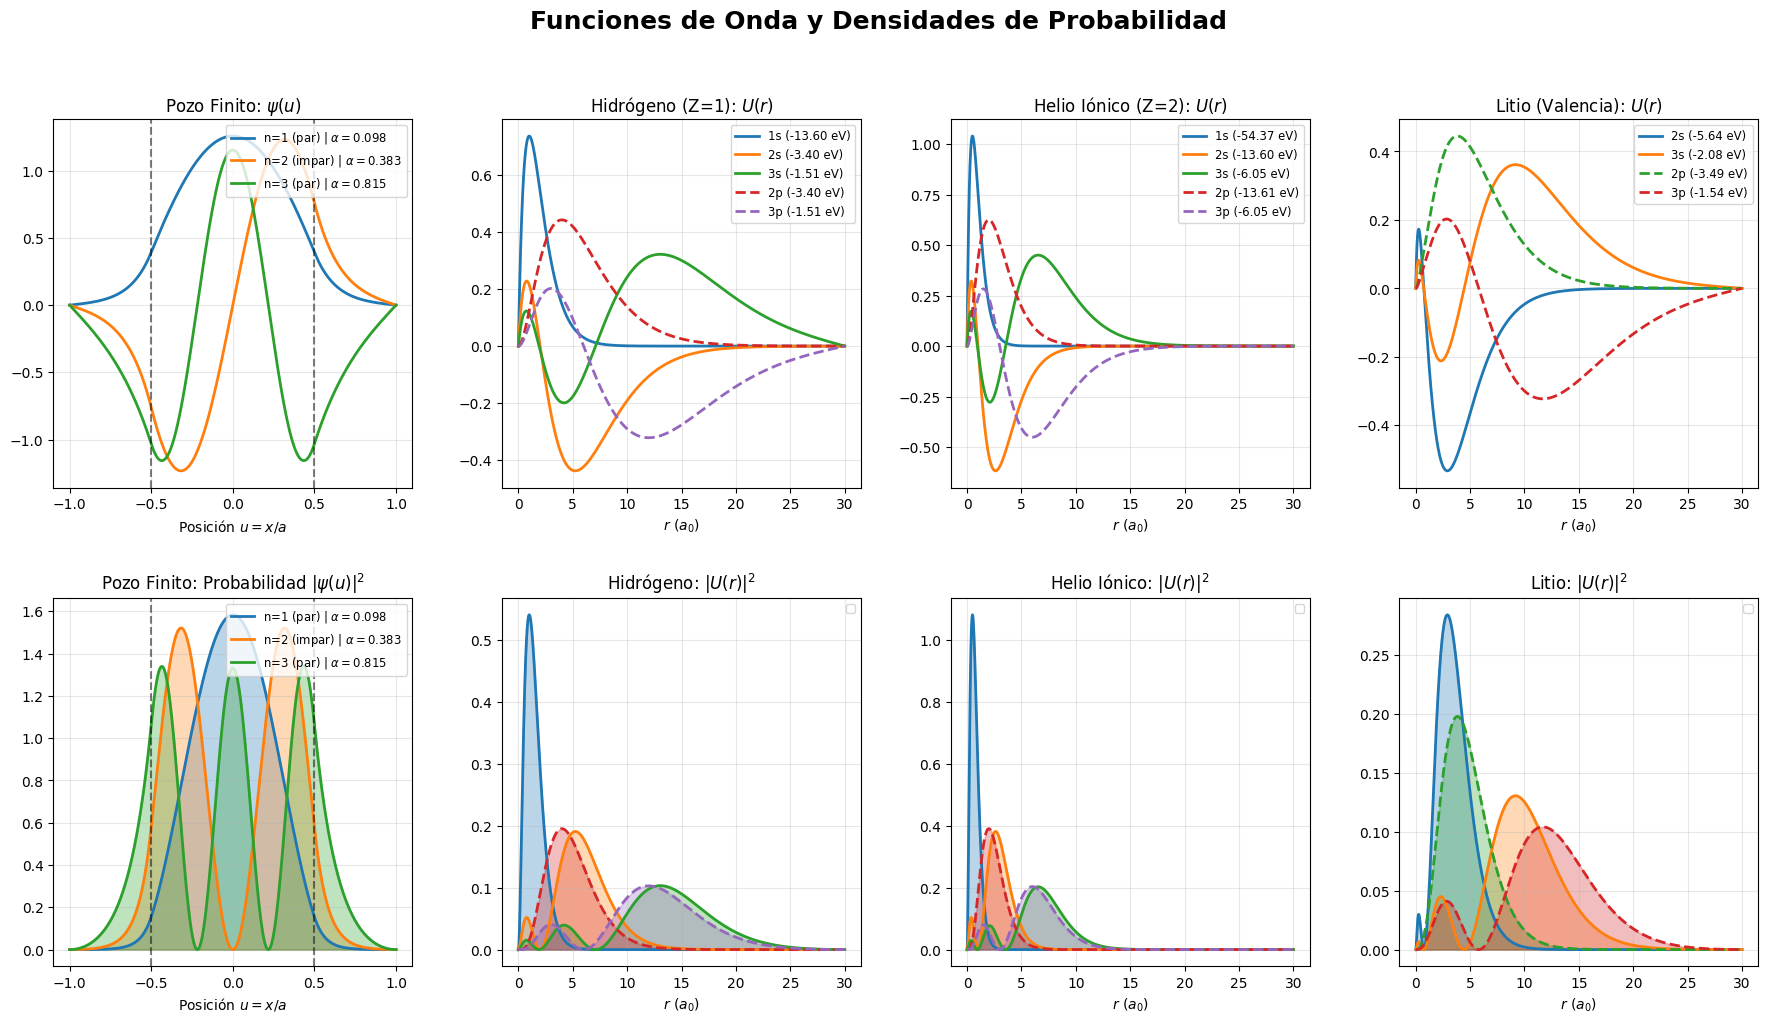
\includegraphics[width=0.9\linewidth]{informe_files/informe_4_2.png}
\end{center}

\section{Discusión de resultados}\label{discusion-conclusiones}

\subsection{Integración de resultados del pozo de potencial}\label{discusion-pozo-integrada}
El análisis del pozo de potencial finito confirma que los dos enfoques numéricos implementados son consistentes en la localización de autovalores, pero no equivalentes en precisión. En la ejecución mostrada, las energías ligadas obtenidas fueron, en eV:

\begin{itemize}
    \item Diferencias finitas explícitas: $E_1 = 23.913685$, $E_2 = 93.437940$, $E_3 = 198.802265$.
    \item Numerov: $E_1 = 23.932411$, $E_2 = 93.525786$, $E_3 = 198.994786$.
\end{itemize}

La cercanía entre ambos conjuntos confirma la robustez del método de disparo con bisección, mientras que la suavidad de las funciones de onda y la estabilidad en el refinamiento de raíces favorecen a Numerov para cálculos de mayor exigencia. Esta ventaja es coherente con el orden de truncamiento: $\mathcal{O}(h^2)$ en diferencias finitas frente a $\mathcal{O}(h^6)$ en Numerov.

Respecto a sensibilidad numérica, los resultados del pozo también muestran tres puntos prácticos:
\begin{enumerate}
    \item La reducción de paso mejora ambos métodos, pero Numerov converge más rápido.
    \item Tolerancias de bisección entre $10^{-8}$ y $10^{-10}$ son adecuadas para autovalores estables.
    \item El dominio $u_{max}$ debe ser suficiente para contener la cola exponencial; valores intermedios (como $u_{max}\approx 4$) equilibran precisión y costo.
\end{enumerate}

Finalmente, al comparar con el límite de pozo infinito, las energías del pozo finito resultan más bajas, como exige la interpretación física: el confinamiento es menos rígido y la función de onda penetra en la región prohibida.

\subsection{Síntesis metodológica}\label{comparativa-metodos}
De forma global, la práctica confirma que ambos métodos son útiles para localizar estados ligados, pero Numerov es el método recomendado cuando se requiere alta precisión con estabilidad numérica. El método explícito por disparo resulta valioso como referencia conceptual y de implementación, mientras que Numerov constituye la opción principal para cálculos sistemáticos.

\subsection{Validación física: hidrógeno, helio y litio}\label{validacion-fisica}
Los resultados para hidrógeno actúan como referencia de control. El estado fundamental $1s$ se obtiene en torno a $-13.60$ eV ($\sim -0.5$ Ha), en excelente acuerdo con la solución analítica. Para los estados $1s$, $2s$, $3s$, $2p$ y $3p$, los errores relativos se mantienen en el rango aproximado $0.004\%$-$0.07\%$, lo que confirma que el esquema numérico reproduce correctamente la estructura hidrogenoide.

Para $He^+$ (núcleo con $Z=2$), los resultados confirman la física esperada: contracción espacial de los orbitales y energías aproximadamente cuatro veces más profundas, coherente con la dependencia $E_n \propto -Z^2$ en sistemas hidrogenoides. En particular, se obtiene $E_{1s}\approx -54.37$ eV, con desviaciones pequeñas respecto al valor analítico.

En litio efectivo, el modelo de apantallamiento rompe la degeneración entre estados con igual $n$ y distinto $l$. En particular, se obtiene $E_{2s} \approx -5.63$ eV, $E_{3s} \approx -2.08$ eV, $E_{2p} \approx -3.49$ eV y $E_{3p} \approx -1.54$ eV. El estado $s$ queda más ligado por su mayor penetración hacia el núcleo, mientras que los estados $p$ están más afectados por la barrera centrífuga y el apantallamiento electrónico.

Estos valores son consistentes con tendencias experimentales (energía de ionización del litio de $5.39$ eV), y las discrepancias restantes reflejan la simplicidad del potencial efectivo adoptado.

\subsection{Factores limitantes y recomendaciones numéricas}\label{limitaciones-recomendaciones}
El principal límite práctico es la sensibilidad a la discretización y al tamaño del dominio. En zonas clásicamente prohibidas, errores pequeños se amplifican exponencialmente, por lo que conviene separar dos objetivos: búsqueda estable de autovalores y extracción física de funciones de onda normalizadas.

Recomendaciones principales:
\begin{enumerate}
    \item Usar pasos pequeños (por ejemplo, $h \sim 10^{-3}$) para mantener precisión en estados bajos y medios.
    \item Ajustar $r_{max}$ o $u_{max}$ según el estado buscado, especialmente para $n$ altos (en hidrogenoides, $r_{max}\sim 30\,a_0$ funciona bien para $n\leq 3$).
    \item Mantener normalización integral $\int |\psi|^2dx = 1$ y controlar la cola numérica en regiones prohibidas para evitar sesgos en la densidad de probabilidad.
\end{enumerate}

\subsection{Comparación entre enfoque analítico y numérico}\label{analitico-vs-numerico}

\begin{table}[H]
    \centering
    \begin{tabular}{|l|c|c|c|c|}
        \hline
        \textbf{Aspecto} & \textbf{Analítico} & \textbf{Dif. Finitas} & \textbf{Numerov} & \textbf{Ventaja} \\
        \hline
        Precisión & Exacta (casos resolubles) & Alta & Muy alta & Analítico \\
        Generalización & Limitada & Alta & Alta & Numérico \\
        Tiempo de cálculo & Muy bajo & Bajo & Bajo & Analítico \\
        Aplicabilidad realista & Baja en sistemas complejos & Alta & Alta & Numérico \\
        \hline
    \end{tabular}
\end{table}

\section{Conclusión}\label{conclusion-integrada}
La práctica confirma que los métodos numéricos son esenciales para estudiar sistemas cuánticos donde no hay solución cerrada. La combinación de disparo y Numerov reproduce correctamente casos analíticos (hidrógeno y $He^+$), permite interpretar fenómenos físicos relevantes (túnel, penetración y apantallamiento) y ofrece una base fiable para abordar problemas más complejos.

La estructura final del trabajo integra teoría, metodología, salida computacional y análisis físico en un flujo único y consistente. En síntesis, este enfoque no solo calcula energías: también aporta comprensión estructural de cómo se organizan los estados cuánticos en sistemas realistas.

\end{document}